\documentclass[a4paper,twoside,12pt]{book}

\usepackage[english]{babel}

\usepackage{fontspec}
\setmainfont{Times New Roman} % Choisissez une fonte sérif lisible (Latin Modern, Junicode, Times)
\usepackage[section]{placeins}
\usepackage{amsmath}
\usepackage{amsfonts}
\usepackage{amssymb}
\usepackage{makecell}
\usepackage{subfigure}
\usepackage{dirtree} 
\usepackage{booktabs}
%Module d'usage facultatif permettant d'intégrer les tables, index, bibliographie, automatiquement à la table des matières
\usepackage{tocbibind}
%\usepackage{lscape}
\setcounter{secnumdepth}{3}
\setcounter{tocdepth}{3} %<--------
\usepackage{caption}
\usepackage{graphicx, multirow,array}
\usepackage{hyperref}
\usepackage{float}
\usepackage{rotating}
\usepackage{etoolbox}

\usepackage{algorithm}
\usepackage{algpseudocode}

\usepackage[margin=2.5cm]{geometry}
\usepackage{setspace}
\setlength{\parindent}{1cm}
\linespread{1.28}

%%%Pour les tableaux
%\usepackage{multirow}


%%% Les index
%\usepackage{makeidx}
%\usepackage{multind} %Ou splitidx
%\usepackage{index} %…
%\makeindex
%\makeindex{edition}
%\makeindex{texte}
%\newindex{etude}{adx}{and}{Index de l'étude}
%\newindex{edition}{bdx}{bnd}{Index de l'édition}



%%%Édition critique
%\usepackage{eledmac}
%\usepackage{eledpar}

%\footparagraph{A}

%\renewcommand{\Rlineflag}{D}

\hyphenation{}


\usepackage[babel]{csquotes}

\usepackage[backend=biber, sorting=nyt, style=enc]{biblatex}
\addbibresource{biblio/memoire_M2.bib}



\usepackage{enumerate,lettrine}

\title{Normes typographiques pour les mémoires}
\author{Francesco Paolo Savatteri}


\begin{document}
	
	
	%\begin{abstract}
	
	%\frontmatter
	
	
	
	\makeatletter
	\def\cleardoublepage{\clearpage\if@twoside \ifodd\c@page\else
		\hbox{}
		\vspace*{\fill}
		\begin{center}
			This page was intentionally left blank.
		\end{center}
		\vspace{\fill}
		\thispagestyle{empty}
		\newpage
		\if@twocolumn\hbox{}\newpage\fi\fi\fi}
	\makeatother
	
	\begin{titlepage}
		\begin{center}
			
			\bigskip
			
			\begin{large}
				UNIVERSITÉ PARIS, SCIENCES \& LETTRES
			\end{large}
			%TODO: nom établissement de préparation
			\begin{center}\rule{2cm}{0.02cm}\end{center}
			
			\bigskip
			\bigskip
			\bigskip
			\begin{Large}
				\textbf{Francesco Paolo Savatteri}\\
			\end{Large}
			
			\bigskip
			\bigskip
			\bigskip
			
			\begin{Huge}
				\textbf{Automatic Detection Of Viral Disinformation Narratives}\\
			\end{Huge}
			\bigskip
			\bigskip
			\begin{LARGE}
				\textbf{A two-task comparative analysis of lightweight neural models}\\
			\end{LARGE}
			
			\bigskip
			\bigskip
			\bigskip
			\begin{large}
			\end{large}
			\vfill
			
			\begin{large}
				Mémoire pour le diplôme de master \\
				« Humanités numériques et computationnelles » \\
				\bigskip
				2025
			\end{large}
			
		\end{center}
	\end{titlepage}
	
	\thispagestyle{empty}
	
	\cleardoublepage
	
	\section*{Abstract}
	\addcontentsline{toc}{chapter}{Abstract}
	\vspace{-0.5em}
	On social media, an enormous amount of disinformation is constantly being produced. Many research works have already explored methods for the automatic detection of fake news. Conversely, much less attention has been devoted to a second, equally crucial aspect in the fight against the spread of disinformation: identifying not only potentially harmful content, but also potentially viral content. Building on this premise, in this work several lightweight neural network architectures were developed and tested on two structurally different textual datasets and across two tasks: fake news detection and online virality prediction. The results show excellent performance of the models in fake news detection, though raising questions about their potential real-world applicability, and encouraging yet still insufficient results in virality prediction.
	
	\medskip
	
	\textbf{Keywords:} Disinformation Detection; Fake News Classification; Social Media Virality Prediction; Imbalanced Classification; Text-based Classification; Lightweight Neural Models; Engagement-Based Features; Multi-features models; FakeNewsNet Dataset; Evons Dataset;
	
	\textbf{Bibliographic Information:} Francesco Paolo Savatteri, \textit{Automatic detection of viral disinformation narratives: a two-task comparative analysis of lightweight neural models}, M.A. thesis « Digital and computational humanities », dir. Florian Cafiero and Chahan Vidal-Gorène, Université Paris, Sciences \& Lettres, 2025.
	
	\vspace{-1em}
	
	\section*{Résumé}
	\addcontentsline{toc}{chapter}{Résumé}
	\vspace{-0.5em}
	Sur les réseaux sociaux, une quantité énorme de désinformation est constamment produite. De nombreux travaux de recherche ont déjà exploré des méthodes pour la détection automatique des fausses nouvelles. En revanche, beaucoup moins d’attention a été accordée à un second aspect, tout aussi crucial dans la lutte contre la propagation de la désinformation : identifier non seulement les contenus potentiellement nuisibles, mais aussi les contenus potentiellement viraux. En partant de ce constat, ce travail a développé et testé plusieurs architectures de réseaux neuronaux sur deux jeux de données textuelles structurellement différents et dans le cadre de deux tâches : la détection de fausses nouvelles et la prédiction de la viralité en ligne. Les résultats montrent d’excellentes performances des modèles pour la détection de fausses nouvelles, tout en soulevant des interrogations quant à leur applicabilité réelle, ainsi que des résultats encourageants mais encore insuffisants en matière de prédiction de la viralité.
	
	\medskip
	
	\textbf{Mots-clés:} Détection de la désinformation; Prédiction de la viralité; Classification déséquilibrée; Classification basée sur le texte; Modèles neuronaux légers; Caractéristiques basées sur l’engagement; Modèles multi-caractéristiques; FakeNewsNet; Evons
	
	\textbf{Informations bibliographiques:} Francesco Paolo Savatteri, \textit{Automatic detection of viral disinformation narratives: a two-task comparative analysis of lightweight neural models}, mémoire de master 2 « Humanités numériques et computationnelles », dir. Florian Cafiero et Chahan Vidal-Gorène, Université Paris, Sciences \& Lettres, 2025.
	
	
	\clearpage
	
	\section*{Acknowledgements}
	\addcontentsline{toc}{chapter}{Acknowledgements}
	
	\vspace{2em}
	
	\begin{flushright}
		\begin{minipage}{0.45\textwidth}
	``Anche le cose vere, gridate e diffuse dagli altoparlanti, assumono apparenza d’inganno''\\
		\mbox{} \hfill \mbox{--- Leonardo Sciascia, \textit{Gli zii di Sicilia}}
		\end{minipage}
	\end{flushright}
	

	\bigskip % spazio verticale prima di iniziare il testo
I would like to thank the professors at the École des Chartes, in particular Florian Cafiero for his enlightening insights and Chahan Vidal-Gorène for the clarity of his thoughts. Outside the classrooms of Rue de Richelieu, I would like to thank Laurent Cordonier for the trust he continues to place in me, which never ceases to amaze me.
	
	
	\clearpage
	\thispagestyle{empty}
	\cleardoublepage
	
	\chapter*{Introduction}
	\addcontentsline{toc}{chapter}{Introduction} \label{intro}
	
	On May 21, 2025, the Oval Office of the White House is crowded with journalists. They have gathered to attend a press conference by the President of the United States, Donald Trump, and his South African counterpart, Cyril Ramaphosa, at the end of an institutional meeting. At a certain point during the event, Trump dims the lights in the room for the screening of a video. The images come from inside the South African Parliament and show the moment when an opposition MP sings a song from the apartheid era, entitled \enquote{Kill the Boer}. The US president then picks up several newspaper photos, which he claims show the graves of a thousand white farmers in South Africa. His goal is to prove the existence of an ongoing genocide against the country's white farmers. \\
	In the days following the episode, various fact-checking services demonstrate that the images used by Trump do not actually represent the events the president believed them to. One of them was not even taken in South Africa, but in Congo\footcite{BBC-2025}. \\
	The so-called white genocide in South Africa is a theory widely spread within far-right circles. On social media, one can very easily find videos and posts supporting this narrative. Searching on X for \enquote{white genocide South Africa}, the results include both posts debunking the theory and posts reinforcing it. The second result that appears is a conspiracy video\footnote{\url{https://x.com/RedPilledGirly/status/1903558156451783064}}, shared by the verified account @TheRedPilledGirl in response to a post by Elon Musk, with a long comment beginning: \enquote{The truth about the genocide taking place in South Africa. Will any human rights groups speak out about what’s happening to infants there?}. The text then continues with phrases such as \enquote{In South Africa, if you're white, you have a target on your back.} On TikTok, searching with the same keywords shows a similar situation: debunking videos are mixed with videos supporting the genocide theory among the very first results. The same applies to Instagram, YouTube, and Facebook. The proportion of fact-checking content decreases exponentially as soon as more alternative platforms, such as Rumble or Odysee, are considered. \\
	
	Let's go back a few months to analyze another episode. In February 2025, Elon Musk reposts an article from the Daily Mail on X. \enquote{Another case of suicidal empathy}, reads the billionaire's post. The article discusses the occupation of the Gaité Lyrique building in Paris by a group of asylum seekers. The article's caption states: \enquote{Left-wing theater managers who invited 200 migrants to a free show will abandon the building and face bankruptcy as refugees still refuse to leave after three months and spark wave of sex-related violence.} The accusation of sexual assaults inside the building has not been confirmed by any of the actors interviewed by fact-checking services that have investigated the case\footcite{pezet}. Despite that, this element is not highlighted in any way under Musk's post, and there is no trace of “community notes,” X's system for verifying fake news. Meanwhile, the post has reached 33 million views.\\
	
	These two relatively recent cases are just the most striking among many other episodes of false information spreading in recent months, not exclusively in right-wing circles\footnote{For example, here is a false quote from Pope Leo XIV that has been widely circulated in progressive circles on the internet: \url{https://x.com/TheRealDKGray/status/1922290861095657477}}. False information is constantly being produced on the internet, mainly on social media, but not exclusively. Some of it is the result of honest mistakes, while other is spread as a joke -- for example, the AI-generated video that went viral of a kangaroo waiting to board a plane, which many thought was real\footnote{\url{https://www.tiktok.com/@yagirlgabby_/video/7509214607869840683}}. Still others are the result of coordinated offensive strategies by malicious actors seeking to influence public debate in entire countries. In a 2023 survey conducted by Ipsos in collaboration with the UN agency UNESCO, 97\% of 8000 people from 16 different countries said they had at least once been misled or influenced by disinformation before finding out it was false in the media or on social media\footcite{ipsos2023}.\\
	
	The development of methods for the automatic identification of fake news, as well as the development of technologies for predicting the virality of different narratives, are therefore fundamental processes for the proper maintenance of global public debate.	It is in this spirit that this work was created.
	
	\section*{The rationale behind this work}
	\addcontentsline{toc}{section}{The rationale behind this work} 
	
	A huge amount of text, images, and videos are produced every moment on social media.  It is not difficult to imagine that with the advent of generative AI, the flow of content is set to increase or has already increased. For institutions, companies, and observers dealing with disinformation, this means having to deal with a huge amount of data to analyze. The activity of these actors can therefore be considered as a large-scale filtering task: among billions of harmless pieces of content, find the harmful ones. And among many harmful pieces of content, find those that are likely to reach a large number of people, as quickly as possible. To simplify as much as possible, two key activities can be identified:
	
	\begin{enumerate}
	\item automatic identification of disinformation content
	\item early identification of viral content
	\end{enumerate}
	
	On the first point, a clarification is needed. The common idea is that disinformation is conveyed by false, invented content. This also applies to academic circles. Many datasets for identifying fake news, for example, use true-false binary classifications to categorize statements or articles. This is not always the case. A telling example is the so called “bedbug psychosis” in France in late 2023\footcite{tf12024}. The underlying phenomenon was real -- a resurgence of bedbug infestations documented by health authorities -- but it was artificially amplified by a coordinated Russian disinformation campaign. False articles and videos, mimicking the style of reputable French media, linked the infestations to Ukrainian refugees or Western sanctions. These pieces were disseminated through networks of fake accounts and websites, boosting their visibility and fuelling public anxiety ahead of the Paris 2024 Olympics and the European elections. In this case, disinformation did not rely on a wholly fabricated event, but on the distortion and exaggeration of a real one. \\
	
	For this reason, any experiment with binary classifications on the truth or falsehood of content should be treated with caution, including this work. In this case, we will still use binary classifications for convenience with respect to the available data. However, it is worth bearing in mind that reality is more complex than this and that any methodology based on categorizations of this type is difficult to apply to the real world. For this reason, in the course of this work, more attention will generally be given to the less trivial activity of predicting the virality of content, which is more applicable to real-world contexts. Precisely in light of the problems associated with binary labels, all experiments predicting virality are carried out on complete datasets containing both real and fake news, in an attempt to simulate real-world data as closely as possible.\\
	
	In conclusion, the rationale behind this work is to explore deep learning methods for the early identification of disinformation narratives and the prediction of their virality. When testing the models and analyzing the results, we will keep in mind their potential for real-world application. In practice, this means considering scenarios with large, continuous data streams that must be processed quickly. Therefore, methods that involve excessively long or computationally heavy processes will be avoided.\label{rationale}
	
	\section*{The structure of this work}
	\addcontentsline{toc}{section}{The structure of this work}
	
	The conceptual structure of this thesis is organized into four main activities, each corresponding to a specific combination of two fundamental dimensions: the dataset employed and the predictive task performed. Two datasets are utilized: Evons and FakeNewsNet. The Evons dataset consists of articles (including title and description) labeled as true or false, along with their engagement metrics on Facebook\footcite{krstovski2022}. In contrast, the FakeNewsNet dataset comprises sequences of tweets sharing a particular article, also accompanied by binary labels indicating the news veracity\footcite{shu2020}. Two predictive tasks are considered: fake news detection and virality prediction. Consequently, each activity consists of a unique combination of dataset (Evons or FakeNewsNet) and prediction task (fake news detection or virality prediction), providing a comprehensive and comparative overview of the experimental results across different conditions. Here below is a visualization of this structure.
	
	\noindent
	\begin{table}[H]
	\begin{tabular}{p{5.5cm} | p{5cm} | p{5cm}}
		& \textbf{Evons Dataset} & \textbf{FakeNewsNet Dataset} \\[0.3em] \hline
		\textbf{Fake News Detection} & Articles labeled true/false & Tweet sequences labeled true/false \\[0.2em]
		\textbf{Virality Prediction} & Articles with engagement data & Tweets with engagement data \\
	\end{tabular}
	\caption{A grid to visualize the conceptual structure of this work} \label{tab:grid}
	\end{table}
	
	\noindent The structure of this work is organized as follows:
	\begin{enumerate}
		\item The next paragraph presents a literature review of recent advancements in the two tasks under consideration (vertical axis of the grid).
		\item The first chapter of the work describes and analyzes the two datasets used (horizontal axis of the grid).
		\item The second chapter outlines the methods and architectures tested.
		\item The third and final chapter presents and discusses the results obtained.
	\end{enumerate}
	
	
	\clearpage
	
	\section*{Related works}
	\addcontentsline{toc}{section}{Related works}
	For an overview of academic progress in this field, it is useful to first analyze the automatic identification of fake news and then the prediction of virality.
	
	\subsection*{Fake news detection}
		\addcontentsline{toc}{subsection}{Fake news detection}
		Recent advances in automatic fake news detection have increasingly emphasized the integration of multiple types of information -- such as textual content, visual cues, user interactions, and network structure -- to improve accuracy and interpretability. Early approaches that relied primarily on linguistic features have been complemented by models capable of jointly learning from article content and its social reception. For example, Ruchansky et al. proposed in 2017 the CSI model, which combines textual analysis via LSTM networks with embeddings of user comments and credibility signals, achieving accuracies of approximately 0.89 and 0.95 on two benchmark datasets\footcite{ruchansky2017}. Two years later, in 2019, Shu et al. introduced dEFEND, a co-attention framework that fuses news content with user comments. In evaluations on the FakeNewsNet dataset (PolitiFact and GossipCop), dEFEND reached 90.4\% accuracy on PolitiFact, substantially outperforming text-only baselines. Furthermore, the model is able to report the key comments used for the classification of the article, allowing for greater explainability and interpretability of the result\footcite{shu2019}. \\
		Parallel developments in natural language processing have allowed transformer-based models, such as BERT and its variants. Kaliyar et al.’s FakeBERT combined BERT embeddings with a convolution-based architecture, achieving strong results (98.90\% accuracy) on the benchmark dataset\footcite{kaliyar2021}. Multimodal transformer models have further extended these capabilities: in July 2025, Lu and Yao designed a residual network with multi-head attention to align textual, visual, and even video information. Across increasing data volumes, it achieves peak scores of 0.977 accuracy, 0.986 precision, 0.969 recall, and 0.924 F1, outperforming baselines such as BERT, RoBERTa, and XLNet\footcite{lu2025}. \\
		
		In addition to content-based analysis, several studies have leveraged the structural patterns by which news spreads through social networks. Graph neural network (GNN) approaches represent news items, users, and engagements as nodes in a graph to exploit relational information. Comparative analyses have shown that \enquote{GNNs offer potential efficiency benefits for resource-constrained scenarios despite their lower predictive performance}, compared to Transformer-based models\footcite{kuntur2024}.  Finally, combinations of graph neural network and transformers models have also been proposed. A study by Rama Moorthy et al. introduces a Dual-Stream Graph-Augmented Transformer that integrates BERT for textual representation and Graph Neural Networks for modeling news propagation structures, enabling context-aware fake news detection. Experiments on the FakeNewsNet dataset show the model achieving 99\% accuracy, outperforming baseline approaches\footcite{ramamoorthy2025}.
		
	\subsection*{Virality prediction}
	\addcontentsline{toc}{subsection}{Virality prediction}
	The task of predicting the virality of news items or narratives can be defined as the forecasting of the eventual reach and speed of dissemination of a given piece of information on online platforms, particularly social media. In operational terms, it is typically framed as the prediction of a quantitative popularity metric (such as the number of shares, retweets, or cascade size) given early-stage diffusion signals. This remains a challenging problem, as virality is influenced by multiple interacting factors, including content characteristics, network topology, temporal dynamics, and stochastic effects. Initial approaches relied on manually engineered features -- for instance, article topic, source reputation, or early view counts -- combined with regression models. More recent research has shifted towards deep learning methods capable of directly learning propagation dynamics from data. \\
	
	One prominent research direction treats information diffusion as a sequential or time-series process. A notable example is DeepCas., an end-to-end deep learning architecture created in 2017, based on Long Short-Term Memory (LSTM) networks that encodes the sequence of resharing events into a latent cascade representation before predicting its future growth\footcite{li2017}. This approach outperformed earlier feature-based baselines. Other works have integrated deep neural architectures with temporal point processes: for example, always in 2017, DeepHawkes augments a Hawkes process with neural feature learning, achieving better performance compared to other baselines, DeepCas included\footcite{cao2017}. More recent advances, such as those by Zhao et al., have employed temporal convolutional networks to model diffusion sequences, achieving competitive results\footcite{zhao2022}. \\
	
	Another approach is to leverage the graph structure of propagation (who-shared-from-whom) and the underlying social network. Topology-aware models represent the diffusion as a tree or subgraph and apply graph learning. For example, the model Topological Recurrent Neural Network (Topo-LSTM) proposed by Wang et al. in 2017 builds a custom RNN that follows the tree of reshares, propagating hidden states along the cascade structure. This Topo-LSTM improved prediction especially for cascades with complex branching. More recent works use standard GNNs: a notable example is Graph Cascade Networks, where a GCN or GraphSAGE is applied to the partial cascade graph to predict its future size. Such models can naturally incorporate network features such as degrees of early adopters and community structure. A relevant example is the GRASS model, which targets two challenges in microscopic cascade prediction: “position-hopping”, where infection relationships are ambiguous, and “branch-independency,” where irrelevant users influence prediction. GRASS combines a GRU-like Attention Unit with a Structural Spreading module based on graph convolutional networks that filters relevant users via structural features. It captures spatiotemporal dynamics more effectively than prior models such as DeepHawkes, obtaining better performances than previous models\footcite{li2024}. \\
	
	In many of the studies reviewed, the prediction of content virality is framed as a regression problem, where the target variable is a continuous measure such as the number of views, shares, or interactions. A common practice in these works is to apply a logarithmic transformation, either directly to the target variable or within the evaluation metric (e.g., mean squared log error). This is done in order to address the heavy-tailed distribution of engagement metrics, where a small number of highly viral items dominate the scale. While this approach can improve overall model stability and predictive accuracy across the full dataset, it may compress the range of extreme values and thus obscure differences in the upper tail of the distribution. As a result, models that perform well under such transformations might not be particularly effective at identifying or ranking truly viral content, which is often the most relevant outcome in practical applications. As will be seen later, this work frames the activity of predicting virality as a classification problem to ensure greater interpretability of the results.
	
	\chapter{Data}
	This section will describe in detail the two datasets used, called Evons and FakeNewsNet.
	
	\section{Evons} \label{evons_pres}
	Evons\footcite{krstovski2022}, introduced at the 29th International Conference on Computational Linguistics, is a curated dataset of news articles from both fake and real news media sources, each paired with the thumbnail image and description used when shared on Facebook. It includes the Facebook engagement count for every article as a proxy for measuring virality. In addition to the full article text, the dataset provides annotations for thumbnail images, including content tags, color attributes, and facial attributes for any detected faces. \\
	
	As the curators explain in the presentation paper, the dataset comprises 92,969 news articles from fake and real news sources published between January 2016 and December 2017, a period chosen for its relevance to the 2016 U.S. Presidential election. Fake news sources were identified by cross-referencing three independently curated lists: Media Bias Fact Check’s “Questionable Sources”, Politifact’s Fake News Almanac and the BS Detector collection. Only outlets appearing on at least two lists were retained, excluding satire, republishers, and post-election launches. This process resulted in six fake news sites, while real news sources were drawn from the “All the News 2.0” dataset, selecting only outlets with high factual reporting and minimal bias. Thumbnail images and descriptions were extracted using the webpreview1 package.\\
	
	In the dataset, virality is measured using Facebook engagement counts. Engagement is the sum of shares, likes, and comments an article received on Facebook. These numbers were retrieved using the Facebook Sharing Debugger (FSD), which provides engagement data for a given URL. One source, USAS, was blacklisted on Facebook. For this case, engagement numbers were collected using BuzzSumo, which also gathers data from FSD. Both tools provide only aggregated counts, with no user information.\\
	
	Finally, thumbnail images were automatically annotated using two platforms. Microsoft Azure is used to detect visual features and color schemes. The authors used Amazon Rekognition to detect faces and annotate them with facial attributes. For object detection, Azure assigns content tags such as objects, animals, scenery, and actions. There are 5,160 distinct tags in total, with some unique to fake or real news. For color analysis, each image is labeled with dominant foreground and background colors, overall dominant colors, an accent color and a black-and-white flag. For facial analysis, Rekognition identifies faces and records attributes such as gender, smile, eyeglasses, mustache, eyes open, brightness, and sharpness. It also labels emotions like happy, sad, angry, calm, and others.
	
	\subsection*{Exploratory analysis}
	\addcontentsline{toc}{subsection}{Exploratory analysis}
	
	Of 92,969 articles in total, 50,193 originate from real news sources and 42,776 from fake news sources. The key variable \textit{fb\_engagements} exhibits a highly skewed distribution with extreme values. On average, an article receives approximately 4,359 interactions, with a very high standard deviation (27,596), indicating substantial variability in content popularity. The median is only 230 interactions, while the 25th percentile is zero, suggesting that a significant proportion of articles receive no engagement at all. The 75th percentile reaches 2,041 interactions, but the maximum observed value exceeds 4.77 million interactions. This means that there is a small number of highly viral articles that disproportionately influence the mean. This distribution reflects a typical pattern of online content dissemination, where most posts attract limited attention while a minority achieve exceptionally wide reach.
	
	\begin{table}[h!]
		\centering
		\caption{Summary statistics for \textit{fb\_engagements}.}
		\vspace{0.5em}
		\begin{tabular}{l r}
			\hline
			Statistic & Value \\
			\hline
			Count & 92,969 \\
			Mean & 4,358.892 \\
			Standard Deviation & 27,595.68 \\
			Minimum & 0 \\
			25th Percentile & 0 \\
			Median (50th Percentile) & 230 \\
			75th Percentile & 2,041 \\
			Maximum & 4,777,733 \\
			\hline
		\end{tabular}
	\end{table}
	
\begin{figure}[htbp]
\centering
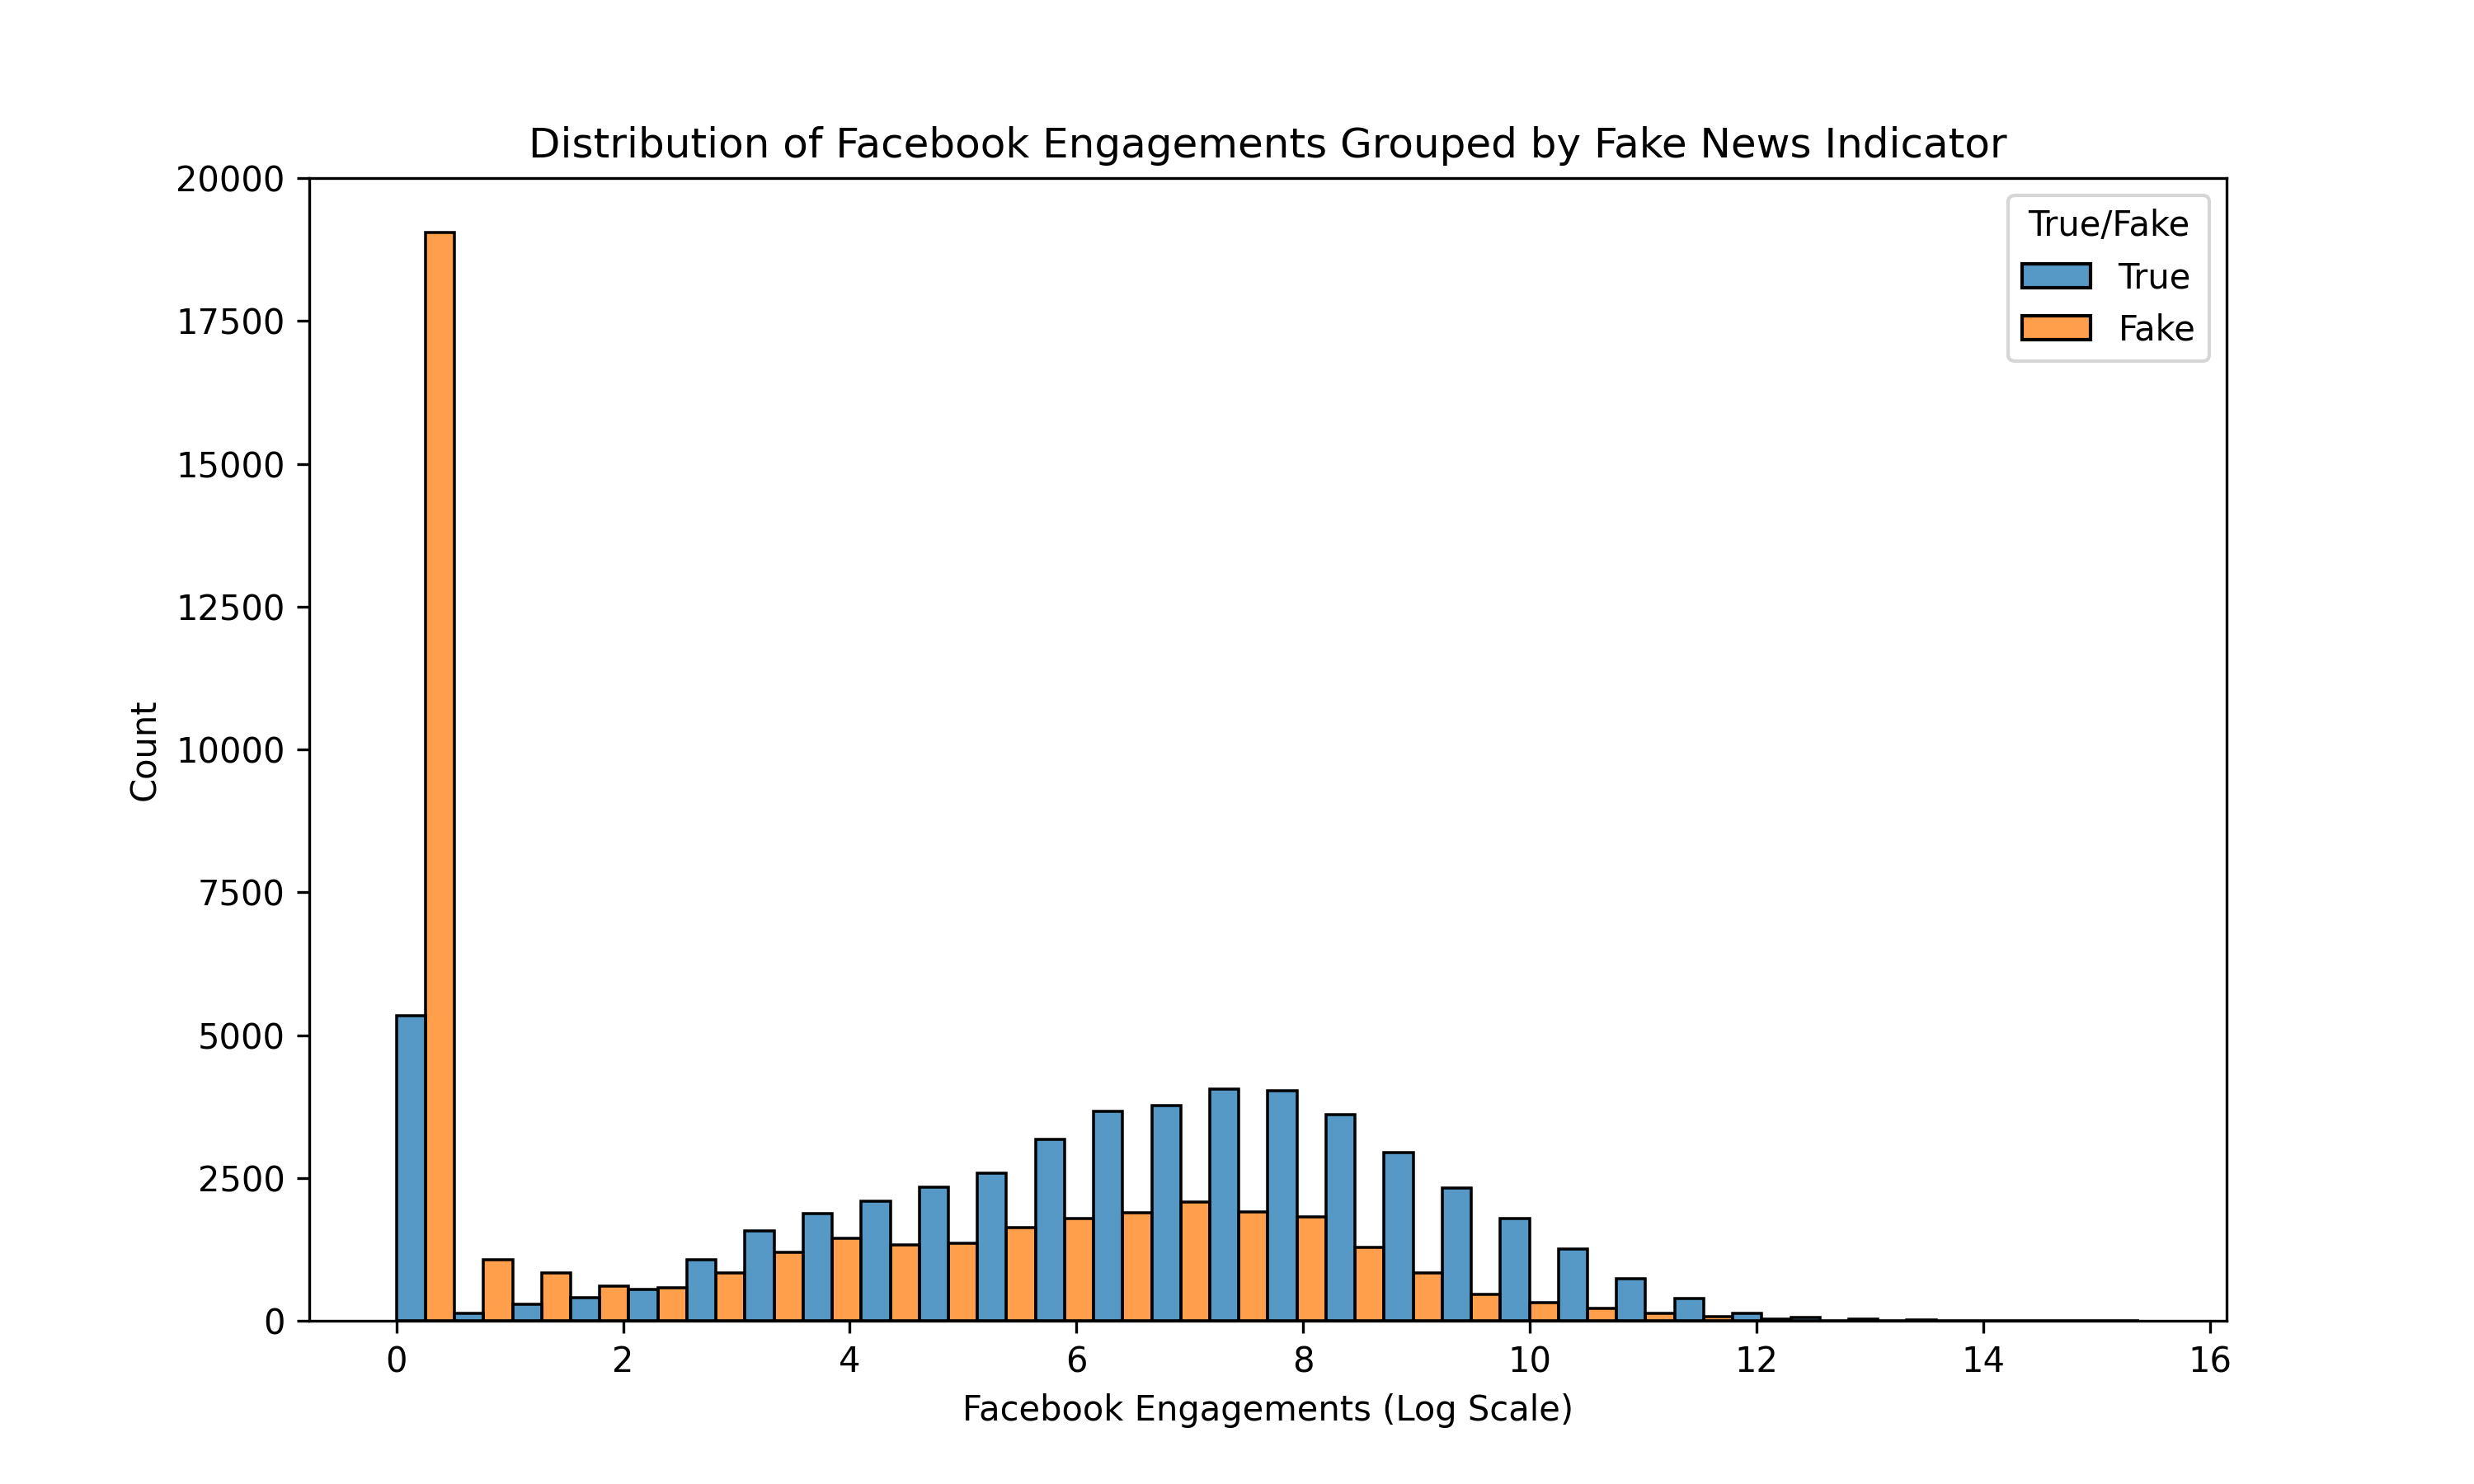
\includegraphics[width=\textwidth]{./img/engagements_by_fake_news.png}
\caption{Distribution of Facebook engagements for articles from true and fake news sources.}
\label{fig:fb_engagements_distribution}
\end{figure}
	
The figure shows the distribution of Facebook engagements for the two categories of articles: those labelled as True and those labelled as Fake. The image reveals a significant structural difference. As shown in Figure~\ref{fig:fb_engagements_distribution}, the distribution for articles from fake sources exhibits a pronounced initial peak in the range of values close to zero, indicating that a substantial share of these articles receives no interactions at all or only a minimal number. Quantitatively, 51.29\% of fake articles register fewer than 10 Facebook engagements, while only 48.71\% exceed this threshold. In contrast, 87.10\% of true articles achieve more than 10 engagements, with just 12.90\% falling below that level. This numerical evidence underscores the stark difference in engagement patterns between fake and true news sources.  

This divergence can be interpreted in light of the nature of the sources included in the dataset. Articles classified as True come from established traditional media, characterized by a consolidated readership base, greater visibility across distribution channels, and a reputation that fosters content sharing. Conversely, articles classified as Fake originate from websites identified as unreliable based on independently curated lists. These are often lesser-known outlets, with more limited audience reach and, in some cases, shorter lifespans.  

This structural difference results in an asymmetric engagement pattern: while articles from both categories can occasionally achieve broad reach, as indicated by the presence of high values in both distributions, the likelihood that an article generates minimal or no interactions is significantly higher for fake sources.\\

\begin{figure}[htbp]
	\centering
	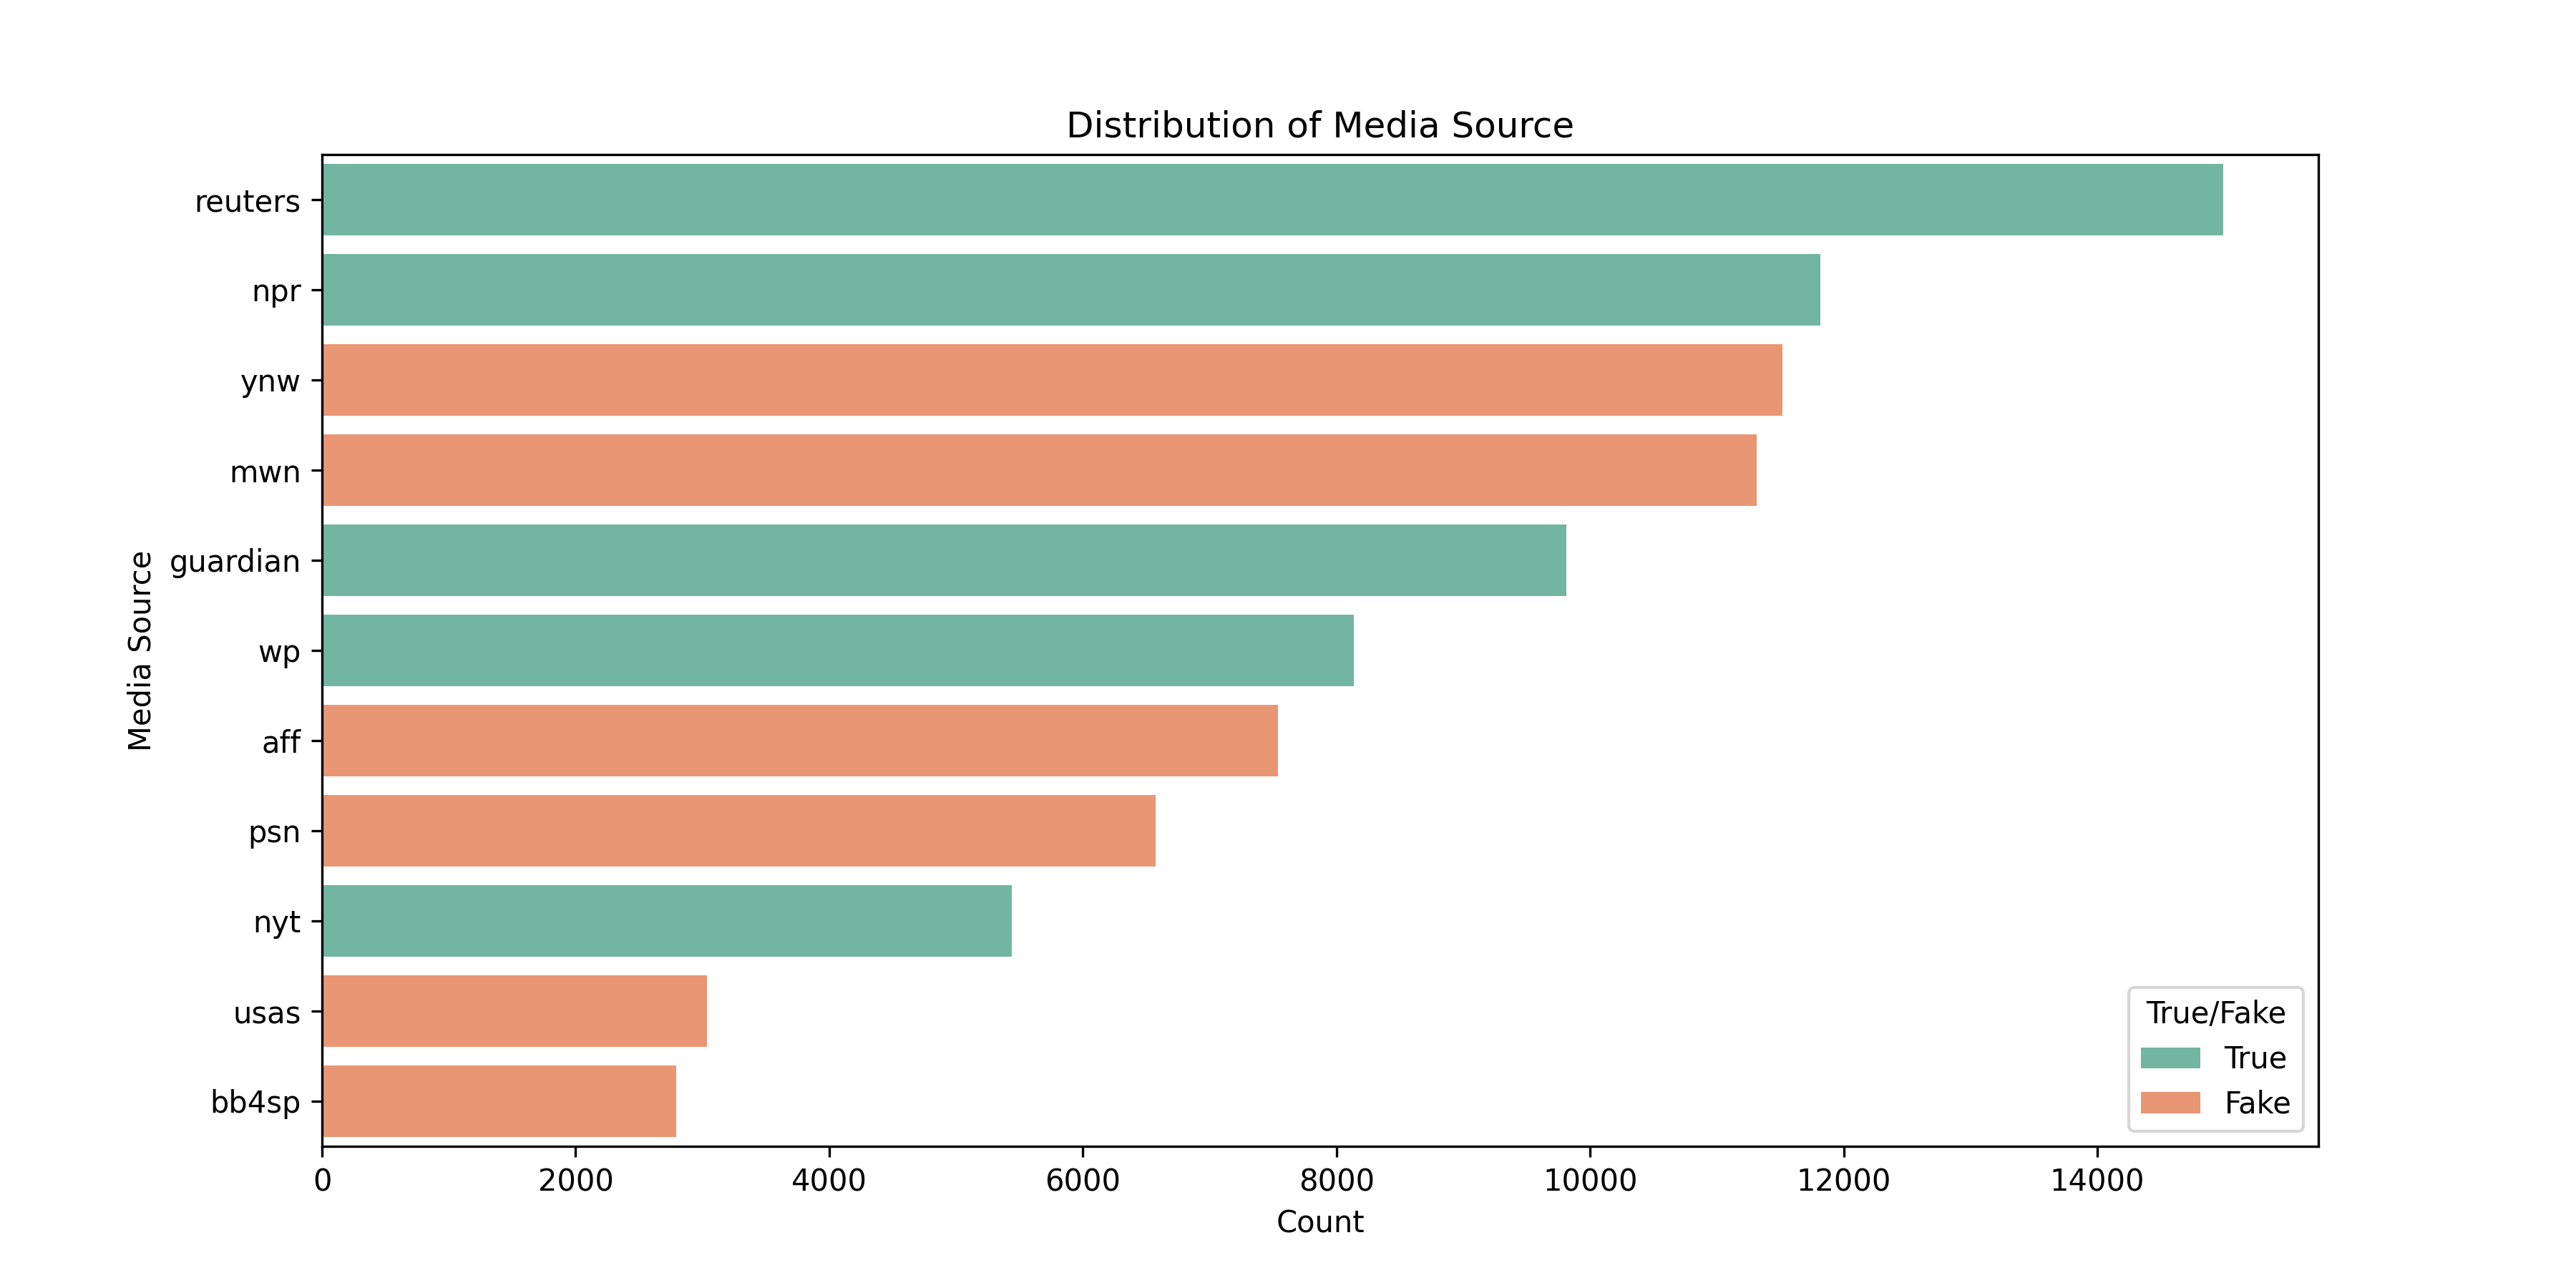
\includegraphics[width=\textwidth]{./img/media_source_distribution.png}
	\caption{Distribution of the sources in the dataset, colored by label}
	\label{fig:sources_count}
\end{figure}

Another useful graph for studying this dataset is shown in Figure~\ref{fig:sources_count}. As can be seen, the two most represented sources are Reuters and NPR, with Reuters having a significant lead over the other sources. It is therefore important to bear in mind that the different sources are not uniformly represented in the dataset, which can obviously affect models' training and validation.

\subsection*{Processing steps}
\addcontentsline{toc}{subsection}{Processing steps}
Due to the nature of the dataset, there was almost no preprocessing to be done. Although each article contained a large amount of multimodal data (e.g., annotated thumbnail images), it was decided to consider only the following fields when testing the different models: 

\begin{table}[h]
	\centering
	\begin{tabular}{cl}
		\hline
		 & \textbf{Variable} \\ \hline
		1 & Title text \\
		2 & Caption text when the article is shared on Facebook \\
		3 & Source (as a categorical variable)  \\
		4 & nb. of \textit{fb\_engagements} (used for labeling) \\
		 \hline
	\end{tabular}
	\caption{Variables used in classification tasks}
\end{table}


It is perfectly plausible that integrating the other data in the dataset could lead to better performance. Despite this, it was chosen to use only the least processed and most accessible data, in order to comply with the underlying criterion of this work already mentioned earlier: the development of pipelines that can be applied quickly, on a daily basis and on a large scale continuous data stream. \\

The only real preprocessing step concerns labels. For more clarity, let the dataset be represented as a collection of articles $\mathcal{A} = \{ a_1, a_2, \dots, a_N \}$ with $N = 92{,}969$, where each article $a_i$ is associated with a tuple of features. That is,
\[
a_i = (t_i, c_i, s_i, e_i), \quad \text{for } i = 1, \dots, N.
\]
The components of each tuple are defined as follows:
\begin{itemize}
	\item $t_i$: the title of article $i$,
	\item $c_i$: the Facebook caption accompanying article $i$,
	\item $s_i$: the source of article $i$,
	\item $e_i$: the number of Facebook engagements for article $i$.
\end{itemize}

The dataset already contains ground-truth labels indicating whether article $a_i$ is true or false. However, for the virality prediction task, we do not have categorical labels but rather a numerical distribution based on the engagement values $e_i$. As previously mentioned, we created binary virality labels $v_i \in \{0,1\}$ based on a quantile threshold. Specifically, let $\tau$ denote the 95th percentile of the distribution $\{ e_1, e_2, \dots, e_N \}$. Then:

$$
v_i = 
\begin{cases}
	1 & \text{if } e_i \geq \tau \quad \text{(viral)} \\
	0 & \text{otherwise} \quad \text{(non-viral)}
\end{cases}
$$

This approach inevitably resulted in a highly unbalanced dataset, with the positive class ($v_i = 1$) accounting for only 5\% of the total records. Clearly, the variable $e_i$ will not be included in the input data fed to the models to avoid an obvious case of data leakage. \label{evons_processing}

\clearpage

\section{FakeNewsNet}
FakeNewsNet\footcite{shu2020} is a public dataset presented in a 2020 paper by Shu et al. It has been widely used by the academic community ever since. It is designed to help researchers study and detect fake news on social media. It combines news articles with their related social media activity, creating a rich source of information for analysis.

\subsection*{Exploratory analysis}
\addcontentsline{toc}{subsection}{Exploratory analysis}

The dataset covers two domains, political news from PolitiFact and entertainment news from GossipCop. PolitiFact evaluates political claims made in news articles and classifies them as true or fake, providing URLs to the original sources. If a source was unavailable, the curators retrieved it from the Wayback Machine or located a matching article using Google search. GossipCop rates entertainment stories on a scale from 0 (fake) to 10 (real), with most ratings below 5 indicating fake stories. Since GossipCop focuses mainly on false stories, true entertainment news is collected separately from E! Online, a reputable media outlet. The dataset's curators then obtained tweets and retweets mentioning the collected news articles, which makes it possible to analyze how such content propagates on social media. \\
In the original presentation paper, the authors conducted an extensive statistical and exploratory analysis to illustrate its richness and potential research applications. They analyzed publisher distributions, finding that fake news frequently originates from a relatively small number of repeat publishers, with certain outlets producing multiple fake stories. In their examination of user profiles, the authors identified statistically significant differences in account creation times between users posting fake versus real news, and, through bot detection using Botometer, they determined that bots are more prevalent in the spread of fake news (approximately 22\%) compared to real news (around 9\%). Here below are a summary table with key statistics on the dataset, an image showing the creation date distribution of users and an image showing the count distribution of followers and followees of users (which, as it is clear from the charts, generally follow a power law distribution). The table and the images have been directly taken from the original FakeNewsNet paper.
\vspace{3em}

\begin{table*}[!htbp]
		\centering
		\resizebox{\textwidth}{!}{%
		\begin{tabular}{| l | l | l | c | c | c | c |}
			\Xhline{3\arrayrulewidth}
			\multirow{2}{*} & \multirow{2}{*} {\textbf{Category}}  &\multirow{2}{*} {\textbf{Features}} & \multicolumn{2}{ c |}{\textbf{PolitiFact}} & \multicolumn{2}{ c |}{\textbf{GossipCop}}   \\ 
			\cline{4-7}
			& & & \textbf{Fake} & \textbf{Real} & \textbf{Fake} & \textbf{Real}  \\
			\Xhline{2\arrayrulewidth}
			
			\multirow{ 3}{*}{\textbf{\makecell{News \\ Content}}} & \multirow{ 2}{*}{\textit{Linguistic}} & \# News articles & 432&  624& 5,323 &  16,817\\ 
			% \cline{3-7}
			
			& & \# News articles with text & 420  & 528 & 4,947 &16,694\\ \cline{2-7}
			& \textit{Visual} & \# News articles with images & 336  & 447 & 1,650 & 16,767\\ \Xhline{3\arrayrulewidth}
			
			\multirow{12}{*}{\textbf{\makecell{Social \\ Context}}}& \multirow{4}{*}{\textit{User}} & \# Users posting tweets & 95,553 & 249,887 & 265,155 & 80,137\\ %\cline{3-7}
			& & \# Users involved in likes &113,473  & 401,363 & 348,852 &145,078\\ %\cline{3-7}
			& & \# Users involved in retweets & 106,195 & 346,459& 239,483 & 118,894\\ %\cline{3-7}
			& & \# Users involved in replies & 40,585 & 18,6675 & 106,325& 50,799\\ \cline{2-7}
			
			& \textit{Post} & \# Tweets posting news& 164,892 &399,237&  519,581& 876,967\\ 
			\cline{2-7}
			&\multirow{ 3}{*}{\textit{Response}}  & \# Tweets with replies & 11,975 &41,852  & 39,717&11,912\\ %\cline{3-7}
			& & \# Tweets with likes & 31692 & 93,839&96,906& 41,889\\ %\cline{3-7}
			& & \# Tweets with retweets & 23,489 &67,035 & 56,552& 24,955\\ \cline{2-7}
			
			
			& \multirow{4}{*}{\textit{Network}} & \# Followers &  405,509,460 &1,012,218,640& 630,231,413& 293,001,487\\ %\cline{3-7}
			& & \# Followees &449,463,557& 1,071,492,603 &619,207,586 & 308,428,225\\ %\cline{3-7}
			& & Average \# followers & 1299.98 & 982.67& 1020.99& 933.64\\ %\cline{3-7}
			& & Average \# followees & 1440.89 & 1040.21 & 1003.14&  982.80\\ \Xhline{3\arrayrulewidth}
			
			\multirow{5}{*}{\textbf{\makecell{Spatiotemporal \\ Information}}}&\multirow{2}{*}{\textit{Spatial}} & \# User profiles with locations  & 217,379 & 719,331& 429,547 & 220,264\\
			&&\# Tweets with locations  & 3,337 & 12,692 & 12,286 & 2,451\\
			\cline{2-7}
			& \multirow{2}{*}{\textit{Temporal}} & \# Timestamps for news pieces & 296 & 167 & 3,558 & 9,119 \\ 
			% & & \# Timestamps for posts &116,005 & 261,262  &  487,327 & 154,383\\ 
			& & \# Timestamps for response &171,301 & 669,641& 381,600 & 200,531 \\ 
			\Xhline{2\arrayrulewidth}
		\end{tabular}%
	}
	\caption{Statistics of the FakeNewsNet repository}
	\label{tab:dataset_stats}
\end{table*}

\begin{figure*}[!h]
	\centering
	\subfigure[PolitiFact dataset]{
		{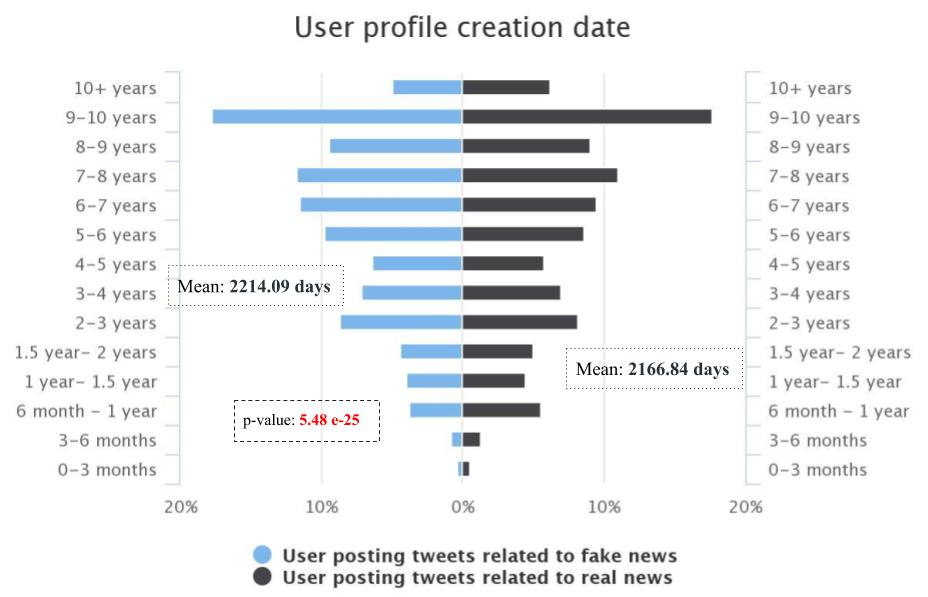
\includegraphics[scale=0.3]{./img/politifact_profile_creation_date.jpg}}
	}
	\subfigure[GossipCop dataset]{
		{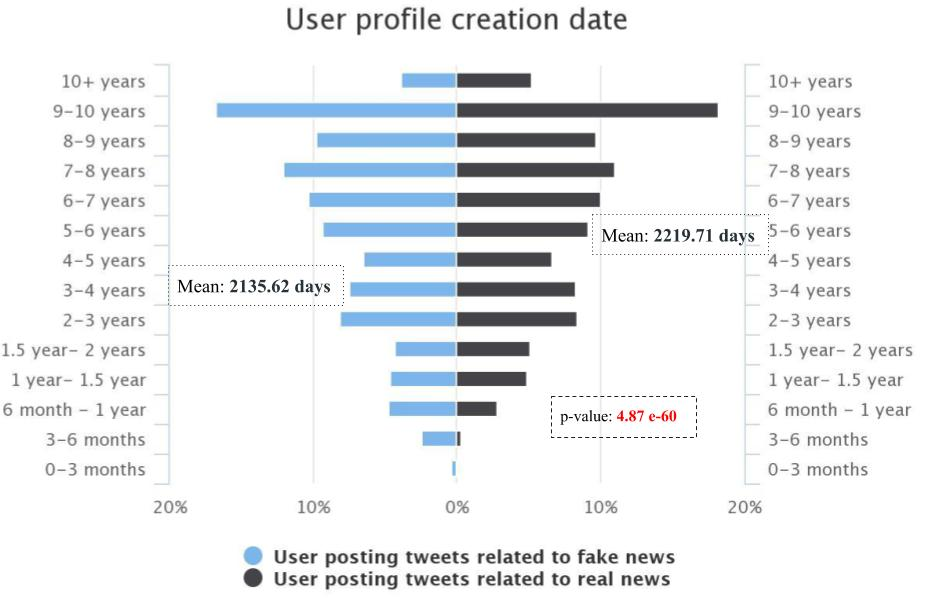
\includegraphics[scale=0.3]{./img/gossipcop_profile_creation_date.jpg}}
	}
	\vskip -0.5em
	\caption{The distribution of user profile creation dates on PolitiFact and GossipCop splits of the dataset}
	\label{fig:user_profile_creation}
	\vspace{-0.1cm}
\end{figure*}

\begin{figure}[!h]
	\centering
	\subfigure[Follower count of users in PolitiFact dataset]{
		{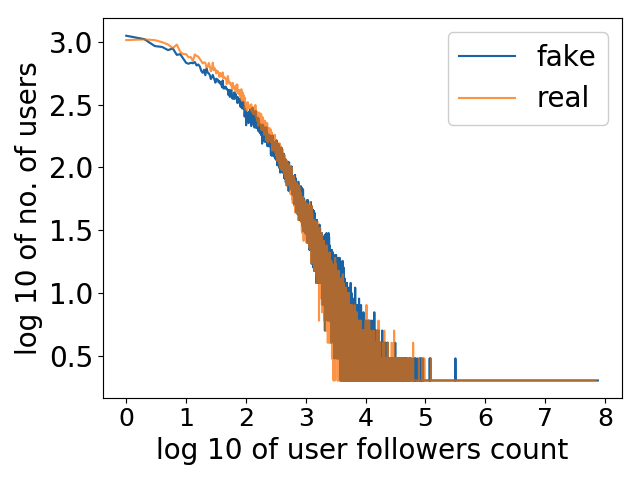
\includegraphics[scale=0.2]{./img/politifact_followers_count.jpg}}
		\label{fig:politifact_follower}
	} \hspace{3em}
	\subfigure[Followee count of users in PolitiFact dataset]{
		{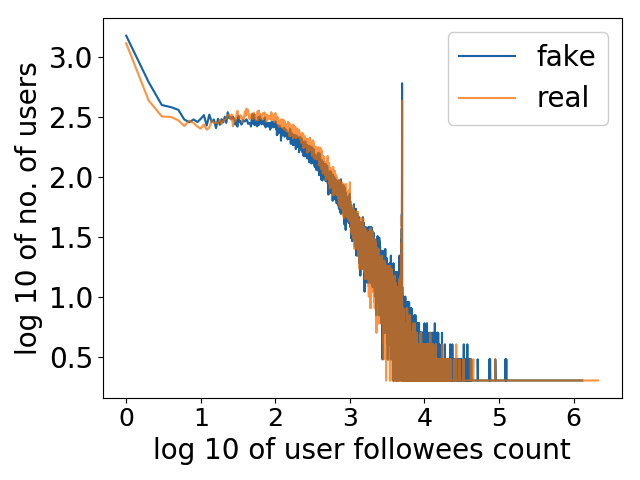
\includegraphics[scale=0.2]{./img/politifact_followee_count.jpg}}
		\label{fig:user_followee}
	} \\
	\subfigure[Follower count of users in Gossipcop dataset]{
		{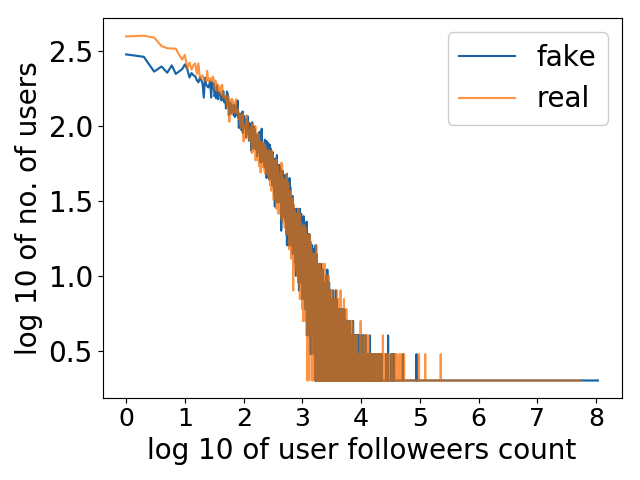
\includegraphics[scale=0.2]{./img/gossipcop_followers_count.png}}
		\label{fig:gossip_follower}
	} \hspace{3em}
	\subfigure[Followee count of users in PolitiFact dataset]{
		{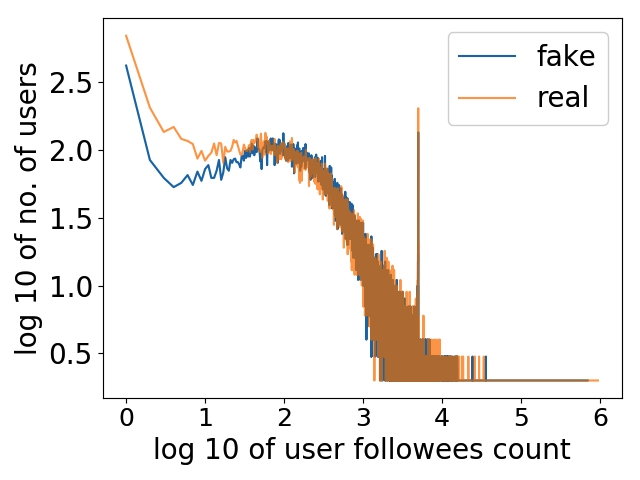
\includegraphics[scale=0.2]{./img/gossipcop_followee_count.jpg}}
		\label{fig:gossip_followee}
	}
	\vskip -0.5em 
	\caption{Distribution of the count of followers and followees related to fake and real news}
	\label{fig:social_network}
	\vspace{-0.1cm}
\end{figure}

\subsection*{Access to data and other issues}
\addcontentsline{toc}{subsection}{Access to data and other issues}

As can be seen in the GitHub repository for the dataset, the data is anonymized: for each tweet, only the unique ID code is shared. Researchers who wish to reuse the dataset must subsequently obtain the raw data -- the text of the tweets and information about their authors -- using the Twitter/X API. This restriction is part of Twitter's privacy policy regarding the use of its data. This did not cause any problems until February 2023, when Twitter/X closed free access to its API, introducing expensive pricing plans. \\
Today, access to this dataset is much more complicated. In the case of this work, it was possible to obtain the Politifact data thanks to the willingness of other members of the academic community who had already worked on the same material in the past. On the contrary, it was not possible to retrieve Gossipcop data. Having obtained the dataset in this way, there are some unverifiable aspects that could influence the data. For example, we do not know when this data was collected via the Twitter API. 

Another problem related to the inability to use the Twitter/X API concerns retweets data: while the statistics on original tweets seem plausible, all retweets have 0 likes. This flaw, probably due to some error in the way the data was collected, clearly creates a problem in processing, requiring all retweets to be discarded and only the original tweets to be worked on. For this reason, the data was processed according to the steps outlined in the following paragraph.
\clearpage

\subsection*{Preprocessing steps}
\addcontentsline{toc}{subsection}{Preprocessing steps}
The dataset files are structured according to the scheme shown here.
\vspace{2em}
\dirtree{%
	.1 politifact.
	.2 fake.
	.3 politifact-1.
	.4 news content.json.
	.4 tweets.
	.5 886941526458347521.json.
	.5 887096424105627648.json.
	.5 \dots.
	.4 retweets.
	.5 887096424105627648.json.
	.5 887096424105627648.json.
	.5 \dots.
	.3 \dots.
	.2 real.
	.3 politifact-2.
	.4 news content.json.
	.4 tweets.
	.4 retweets.
	.3 \dots.
}
\vspace{2em}

The JSON files inside the \textit{tweets} folders contain individual tweet objects, while files in the \textit{retweets} folders contain lists of retweets associated with specific tweets. Based on this structure, the data was processed to reconstruct propagation paths for each news item. However, due to limitations in the retweet data, the propagation paths were built exclusively from original tweets.

Specifically, for each article in the \textit{politifact-n} folder, all corresponding tweets in the \textit{tweets} subfolder were extracted and aggregated into a list. As a result, we obtained a collection $\mathcal{T} = \{ S_1, S_2, \dots, S_N \}$ of propagation paths, where each $S_i$ represents a sequence of tweets associated with a given news article. In total, we constructed $N = 578$ tweet series, each of variable length $n_i = |S_i|$ (i.e., the number of tweets in series $S_i$).

A limitation of this work lies in the relatively small number of reconstructed paths, due to the exclusion of retweets. For comparison, if we had built the paths on retweets instead of tweets, we would have over 65,000 sequences. Within each series $S_i$, the tweets were sorted chronologically according to their publication timestamps, resulting in temporally ordered sequences. Additionally, for each series, the veracity label (Fake or Real) associated with the corresponding article was extracted and linked to the entire series.\\

Below is a descriptive summary table, along with the empirical distribution and log-transformed distribution of the lengths $n_i$ of the tweet series, separately for true and fake articles.


\begin{figure}[h!]
	\centering
	
	\subfigure[Raw distribution]{
		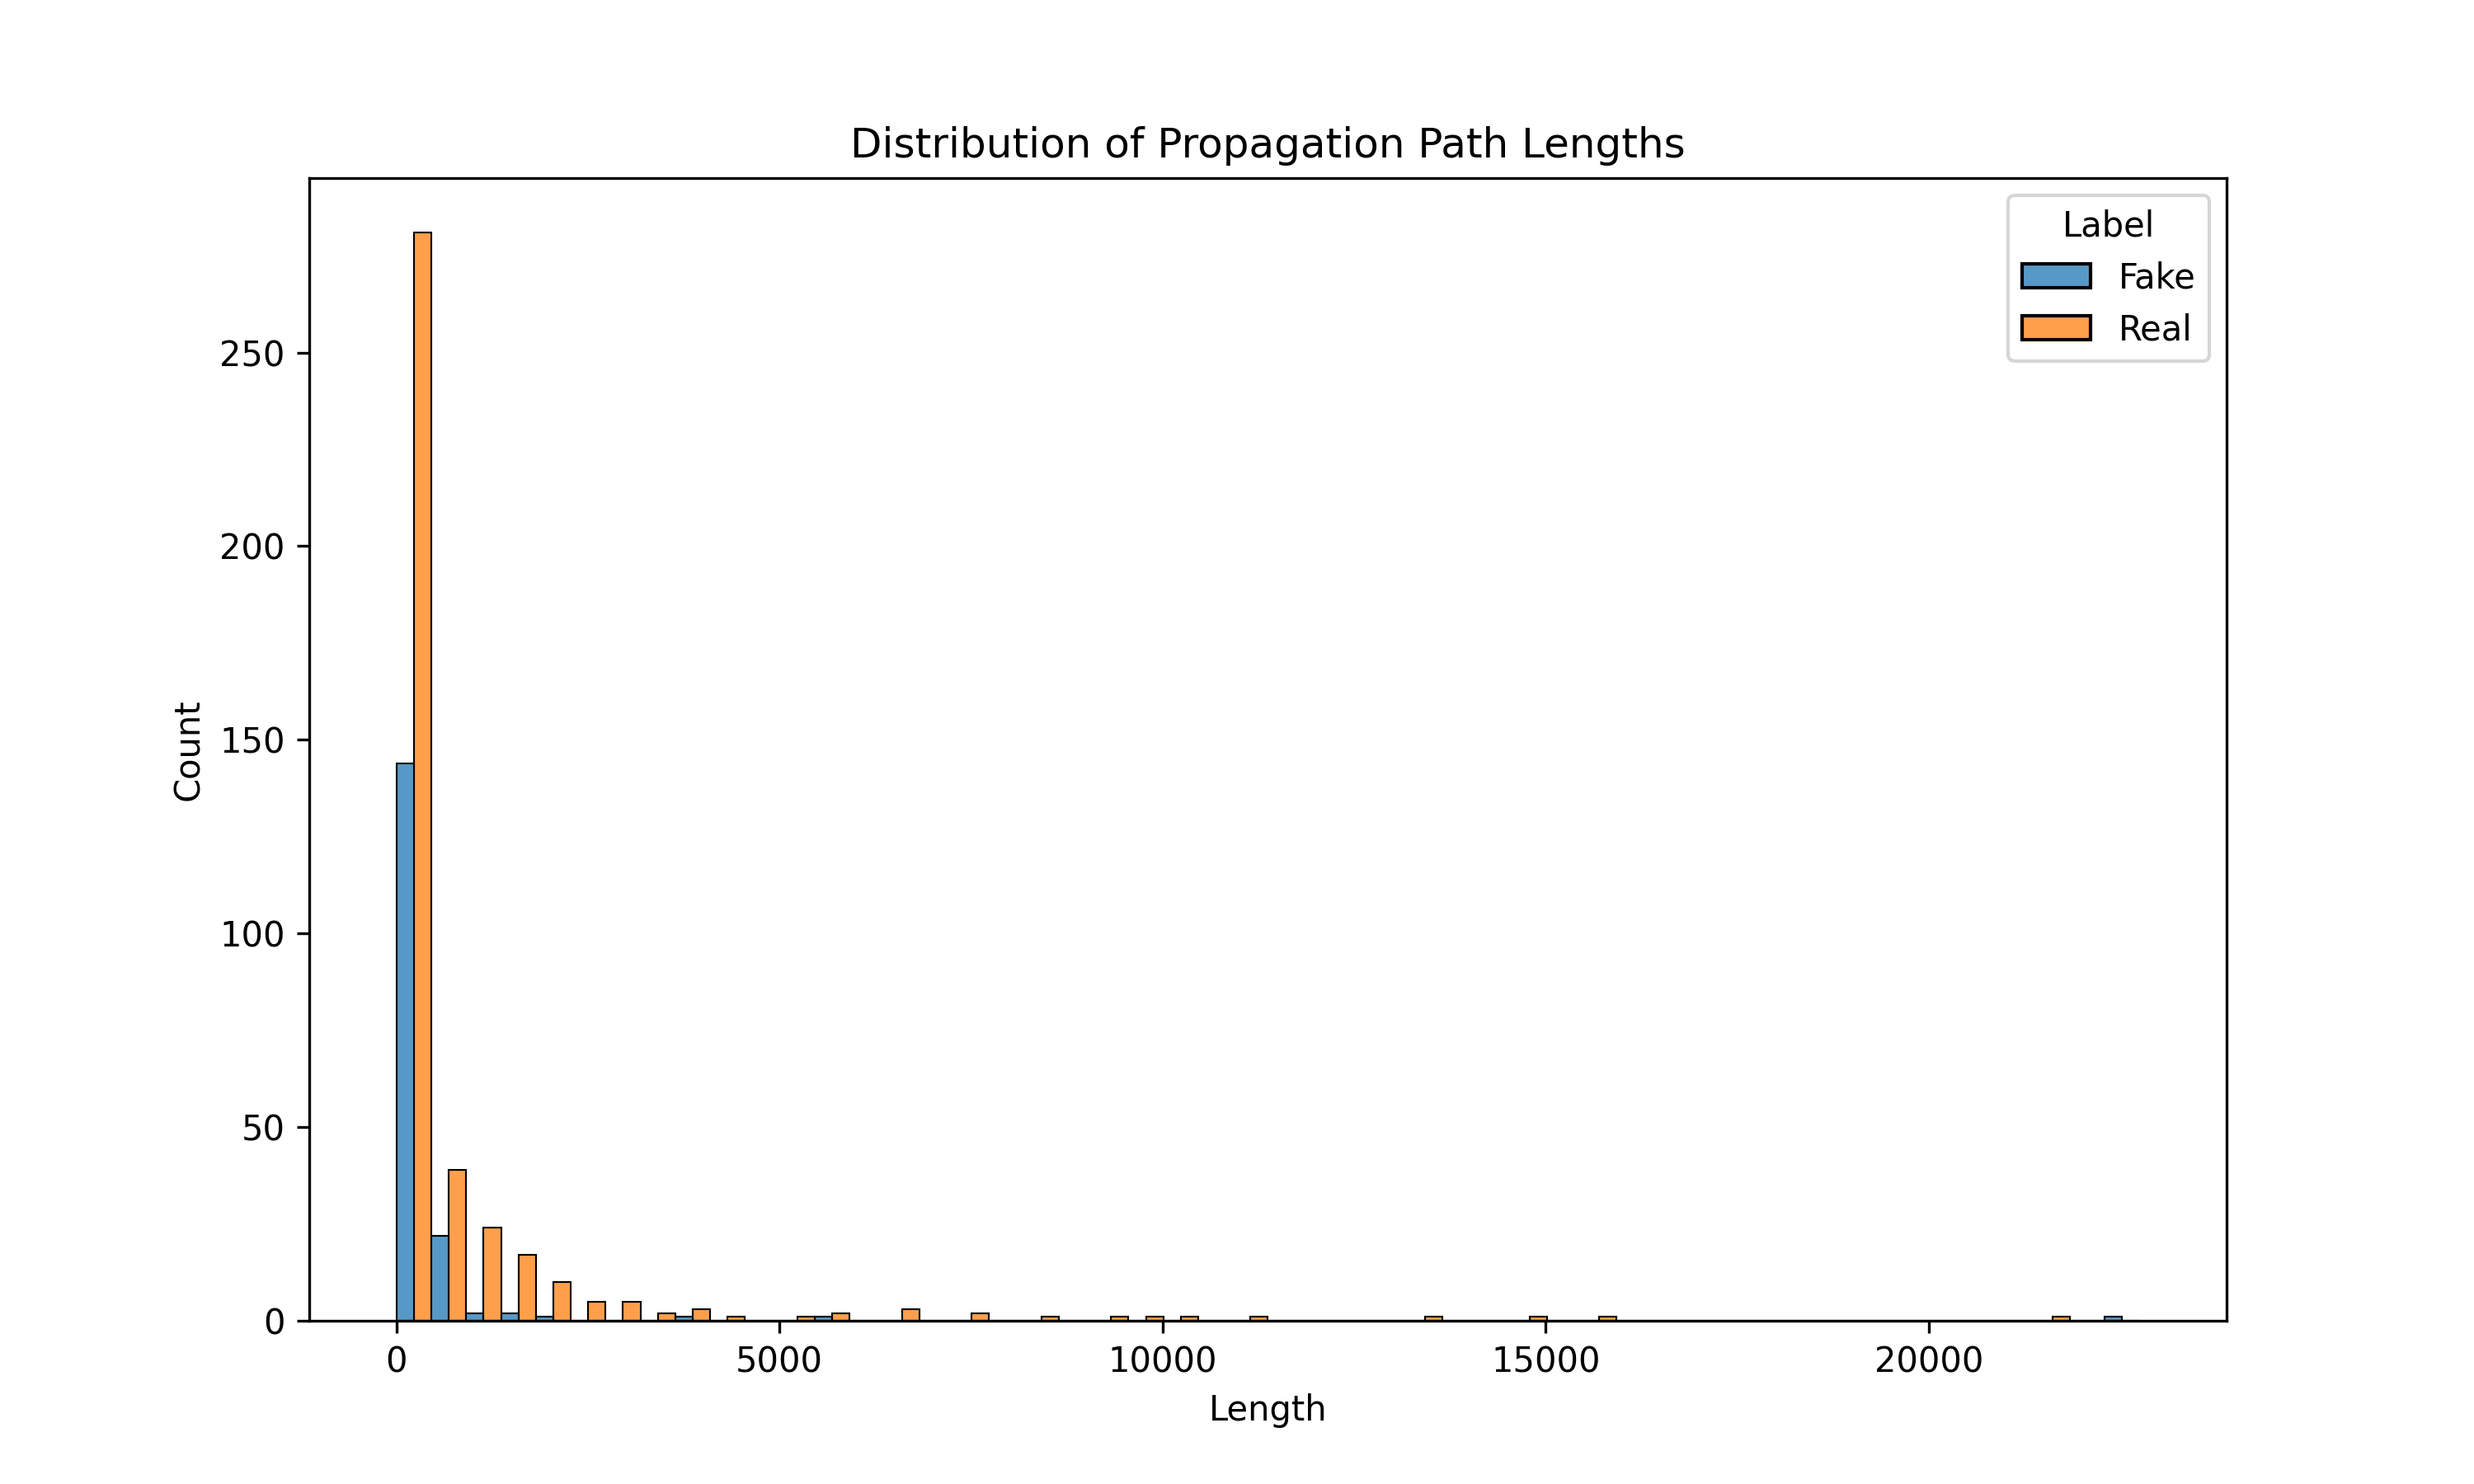
\includegraphics[width=0.8\textwidth]{./img/propagation_path_lengths.png}
		\label{fig:distr_paths}
	}
	
	\vspace{0.5cm} % Optional vertical space between subfigures
	
	\subfigure[Log-transformed distribution]{
		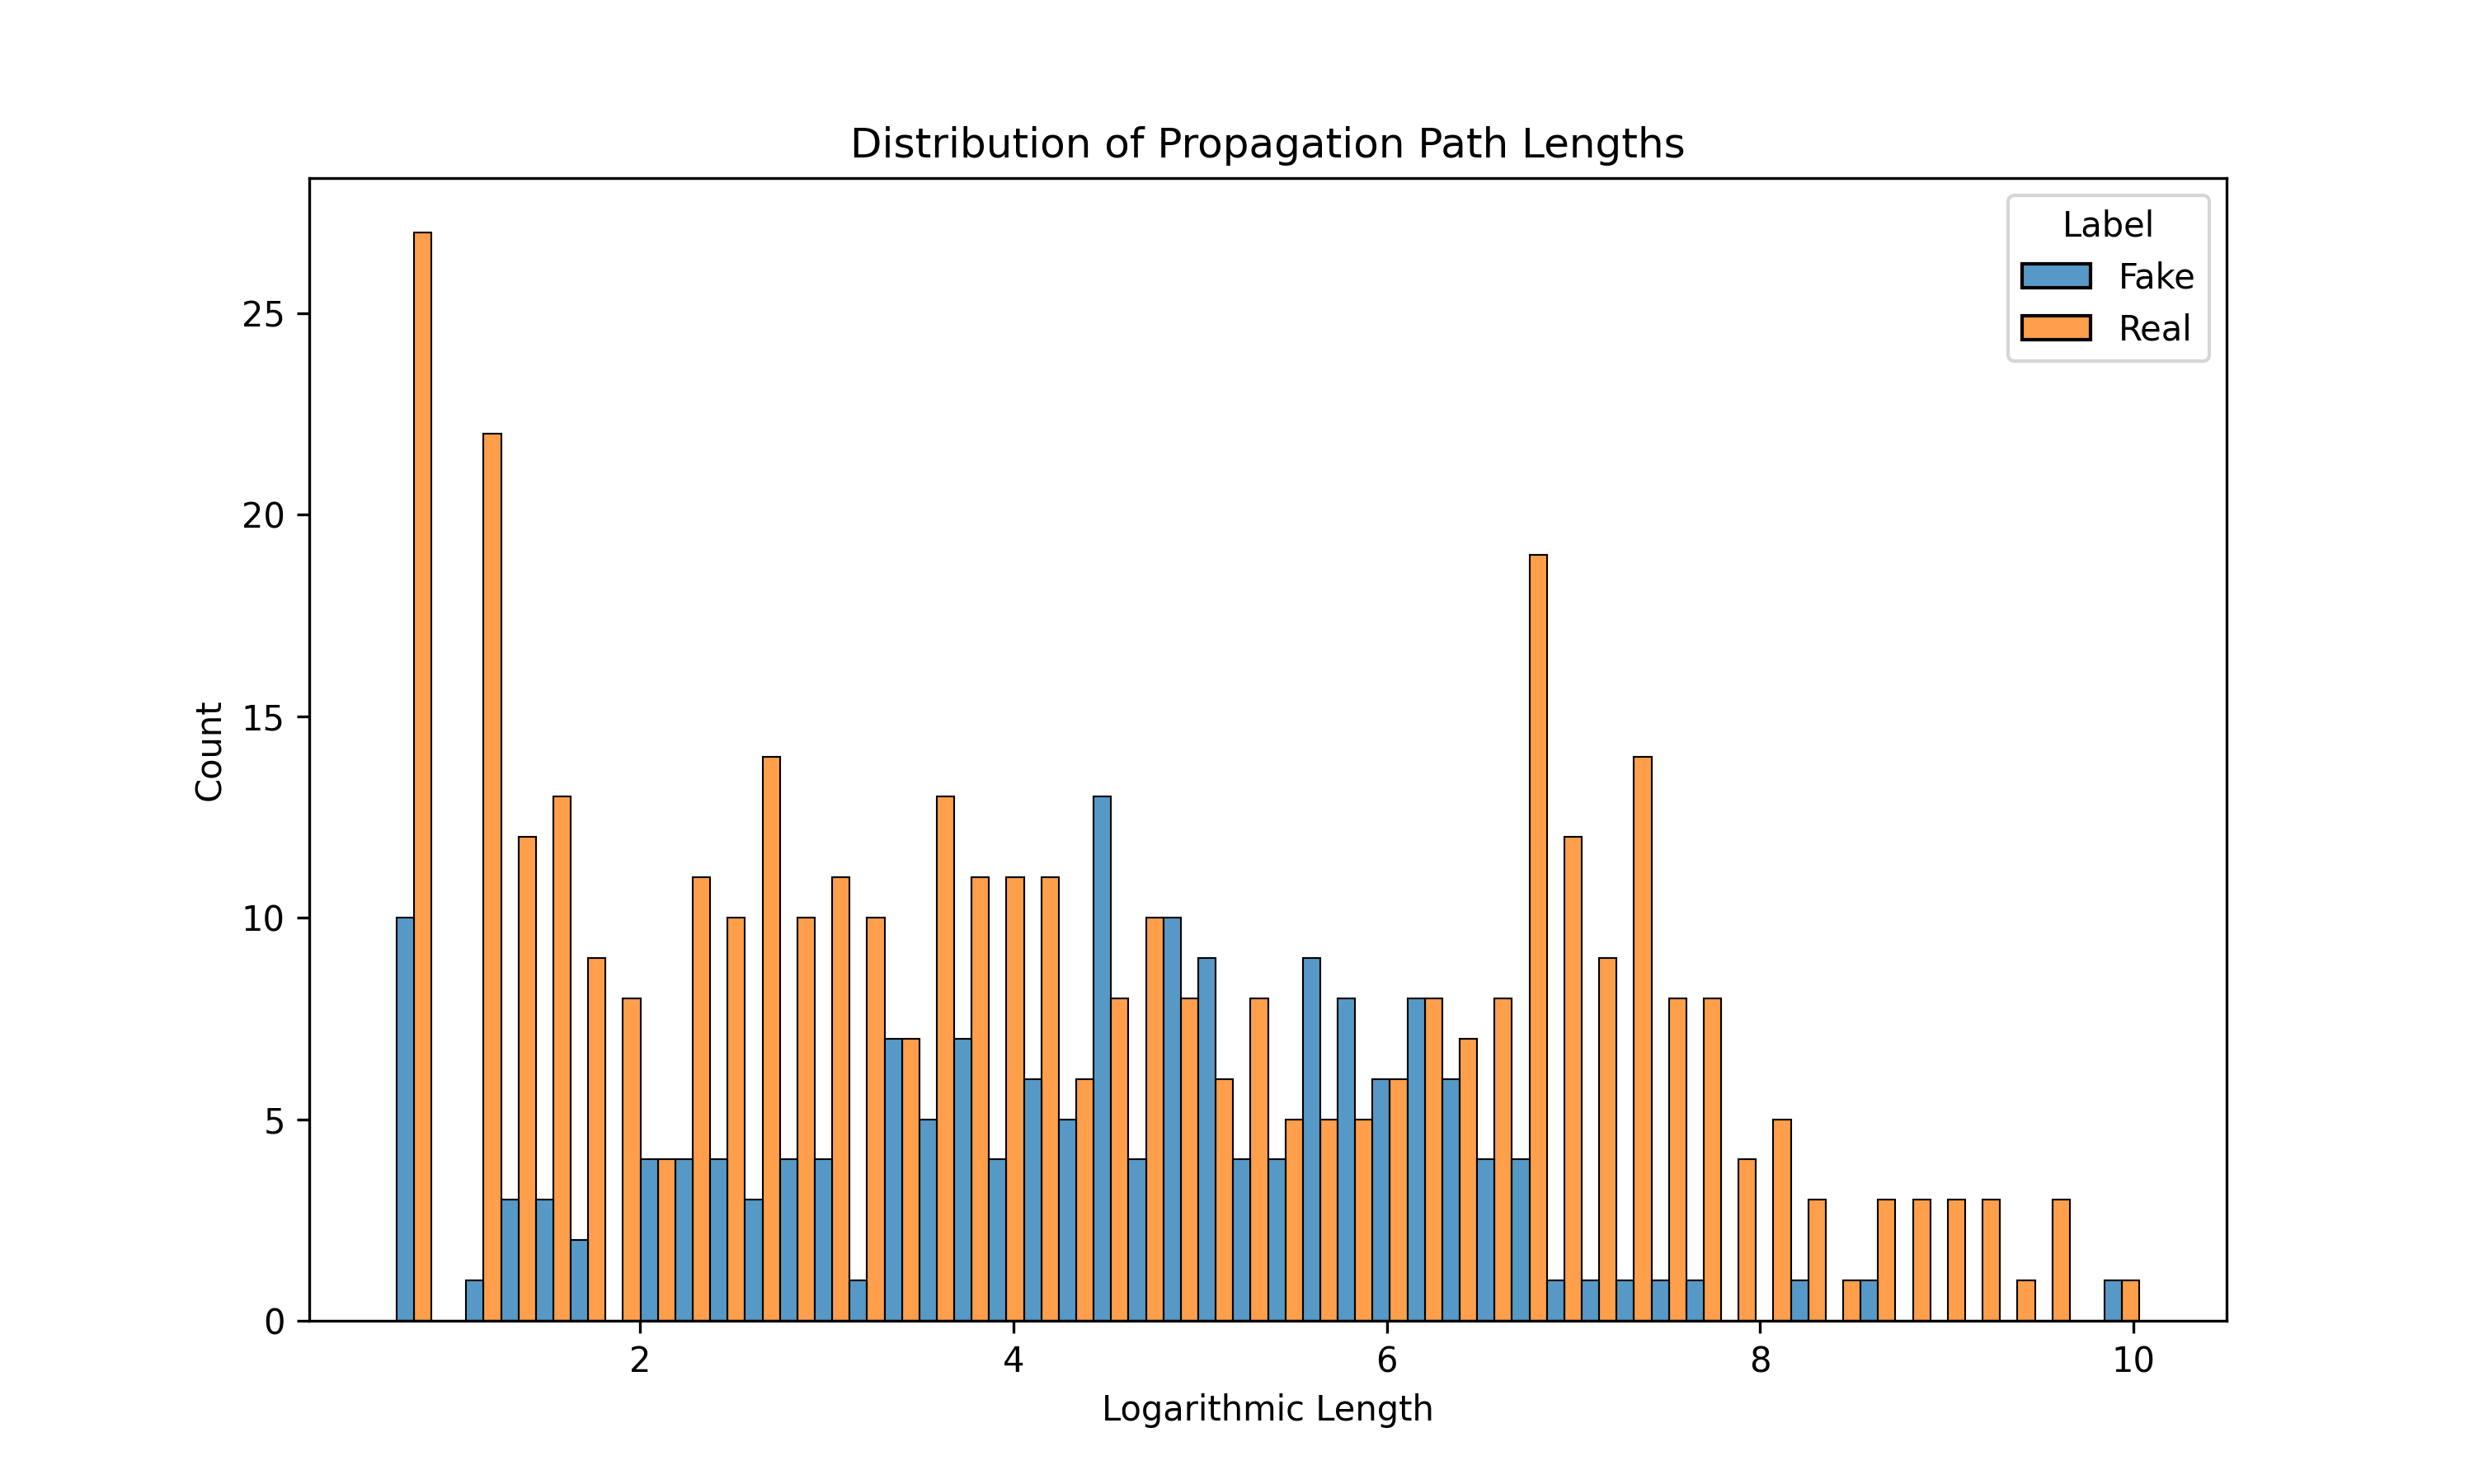
\includegraphics[width=0.8\textwidth]{./img/propagation_path_log_lengths.png}
		\label{fig:log_distr_paths}
	}
	
	\caption{Distributions of propagation path lengths for fake and real news (original and log-transformed).}
	\label{fig:combined_paths}
\end{figure}

\begin{table}[h!]
	\centering
	\begin{tabular}{lcccccccc}
		\toprule
		Label & Count & Mean & Std & Min & 25\% & 50\% & 75\% & Max \\
		\midrule
		Fake & 174.0 & 400.523 & 1803.121 & 1.0 & 27.0 & 94.5 & 309.50 & 22750.0 \\
		Real & 404.0 & 821.777 & 2189.885 & 1.0 & 8.0 & 56.0 & 759.25 & 21497.0 \\
		\bottomrule
	\end{tabular}
	\caption{Descriptive statistics of propagation path lengths for Fake and Real labels.}
	\label{tab:stats_prop_paths}
\end{table}

The number of tweets per news item is highly variable in both classes, with distributions skewed by a small number of articles receiving exceptionally high engagement. On average, true news items attract roughly twice as many tweets as fake ones, though the median values suggest that most articles in both classes receive relatively limited attention. The higher upper quartile for true news indicates that a larger portion of these articles achieve substantial propagation compared to fake news.

Each tweet in the data is a json object following the format mentioned the Twitter/X API documentation\footnote{\url{https://developer.x.com/en/docs/x-api/v1/data-dictionary/object-model/tweet}}. For each tweet, we extracted the data contained in table ~\ref{tab:variables_net}. 

\vspace{2em}

\begin{table}[h!]
	\centering
	\begin{tabular}{cl}
		\hline
		 & \textbf{Variable} \\ \hline
		1 & Tweet text \\
		2 & Creation date and time \\
		3 & Username of the author (retrieved for clarity, not actually used) \\
		4 & Author's user ID (retrieved for clarity, not actually used) \\
		5 & Number of author's followers \\
		6 & Number of author's followings \\
		7 & Author is verified or not (binary variable) \\
		8 & Number of likes \\ \hline
	\end{tabular}
	\vspace{1em}
	\caption{Variables used in classification tasks} \label{tab:variables_net}
\end{table}

Each tweet $T_{ij} \in S_i$ is thus represented as a feature vector:

$$
T_{ij} = \left( \text{text}_{ij},\ \text{time}_{ij},\ \text{followers}_{ij},\ \text{following}_{ij},\ \text{verified}_{ij},\ \text{likes}_{ij} \right)
$$

The second variable in Table ~\ref{tab:variables_net} is the creation timestamp $\text{time}_{ij}$. Since our focus is on the speed of propagation of news rather than the absolute time of tweet publication, we transformed the temporal data into a relative delay format, specific to each propagation path.

For each tweet series $S_i$, we defined the time of publication of the first tweet as the temporal origin:

$$
\text{time}_i^{(0)} = \text{time}_{i1}
$$

For all tweets $T_{ij} \in S_i$, we then computed the temporal delay:

$$
\Delta t_{ij} = \text{time}_{ij} - \text{time}_i^{(0)}
$$

By construction, the first tweet in each series satisfies $\Delta t_{i1} = 0$. The temporal information used in our analysis is therefore represented by $\Delta t_{ij}$, which expresses the delay from the initial tweet of the sequence. This transformation allows for the analysis of propagation dynamics independently of absolute posting times. 

\pagebreak

Finally, with regard to labels, we followed the following procedures. The fake and true labels are necessary for fake news detection and are already present in the dataset. For virality prediction, on the other hand, the total number of likes for each propagation path was calculated. Specifically, for each tweet series $S_i = \{ T_{i1}, T_{i2}, \dots, T_{in_i} \}$, we defined the total number of likes as:

$$
L_i = \sum_{j=1}^{n_i} \text{likes}_{ij}
$$

where $\text{likes}_{ij}$ is the number of likes received by tweet $T_{ij}$. This scalar value $L_i$ serves as a proxy for the virality of the series $S_i$. Here below is a descriptive table of the total likes distribution. \\

\begin{table}[h!]
	\centering
	\begin{tabular}{lcccccccc}
		\toprule
		Label & Count & Mean & Std & Min & 25\% & 50\% & 75\% & Max \\
		\midrule
		Fake & 174.00 & 1,573.24 & 12,896.25 & 0.00 & 7.25 & 46.50 & 295.25 & 168,963.00 \\
		Real & 404.00 & 10,215.90 & 35,499.35 & 0.00 & 0.00 & 19.50 & 1514.75 & 260,698.00 \\
		\bottomrule
	\end{tabular}
	\caption{Descriptive statistics of propagation path total likes for Fake and Real labels.}
	\label{tab:stats_likes_paths}
\end{table}

The number of likes per path varies greatly within both classes. Distributions are extremely skewed by some articles receiving a really high engagement, as for paths' lengths distributions. On average, true news items garner substantially more likes than fake ones. However, the median values reveal that most articles receive relatively modest levels of appreciation, particularly in the real news category. The markedly higher upper quartile for real news suggests that a greater share of these articles achieve significant audience endorsement compared to fake news. At the same time, the 25\% quartile for real news is 0, showing that many paths based do not get any likes at all. That is also confirmed by a higher standard deviation for real news paths. \\

As shown in graph ~\ref{fig:corr_likes_len}, there is a strong correlation between the length of propagation paths and the total number of likes. It is easy to understand why this is the case, as more tweets associated to a specific article suggest it might be a more trending topic that could more easily go viral. 

\pagebreak

\begin{figure}[h!]
	\centering
	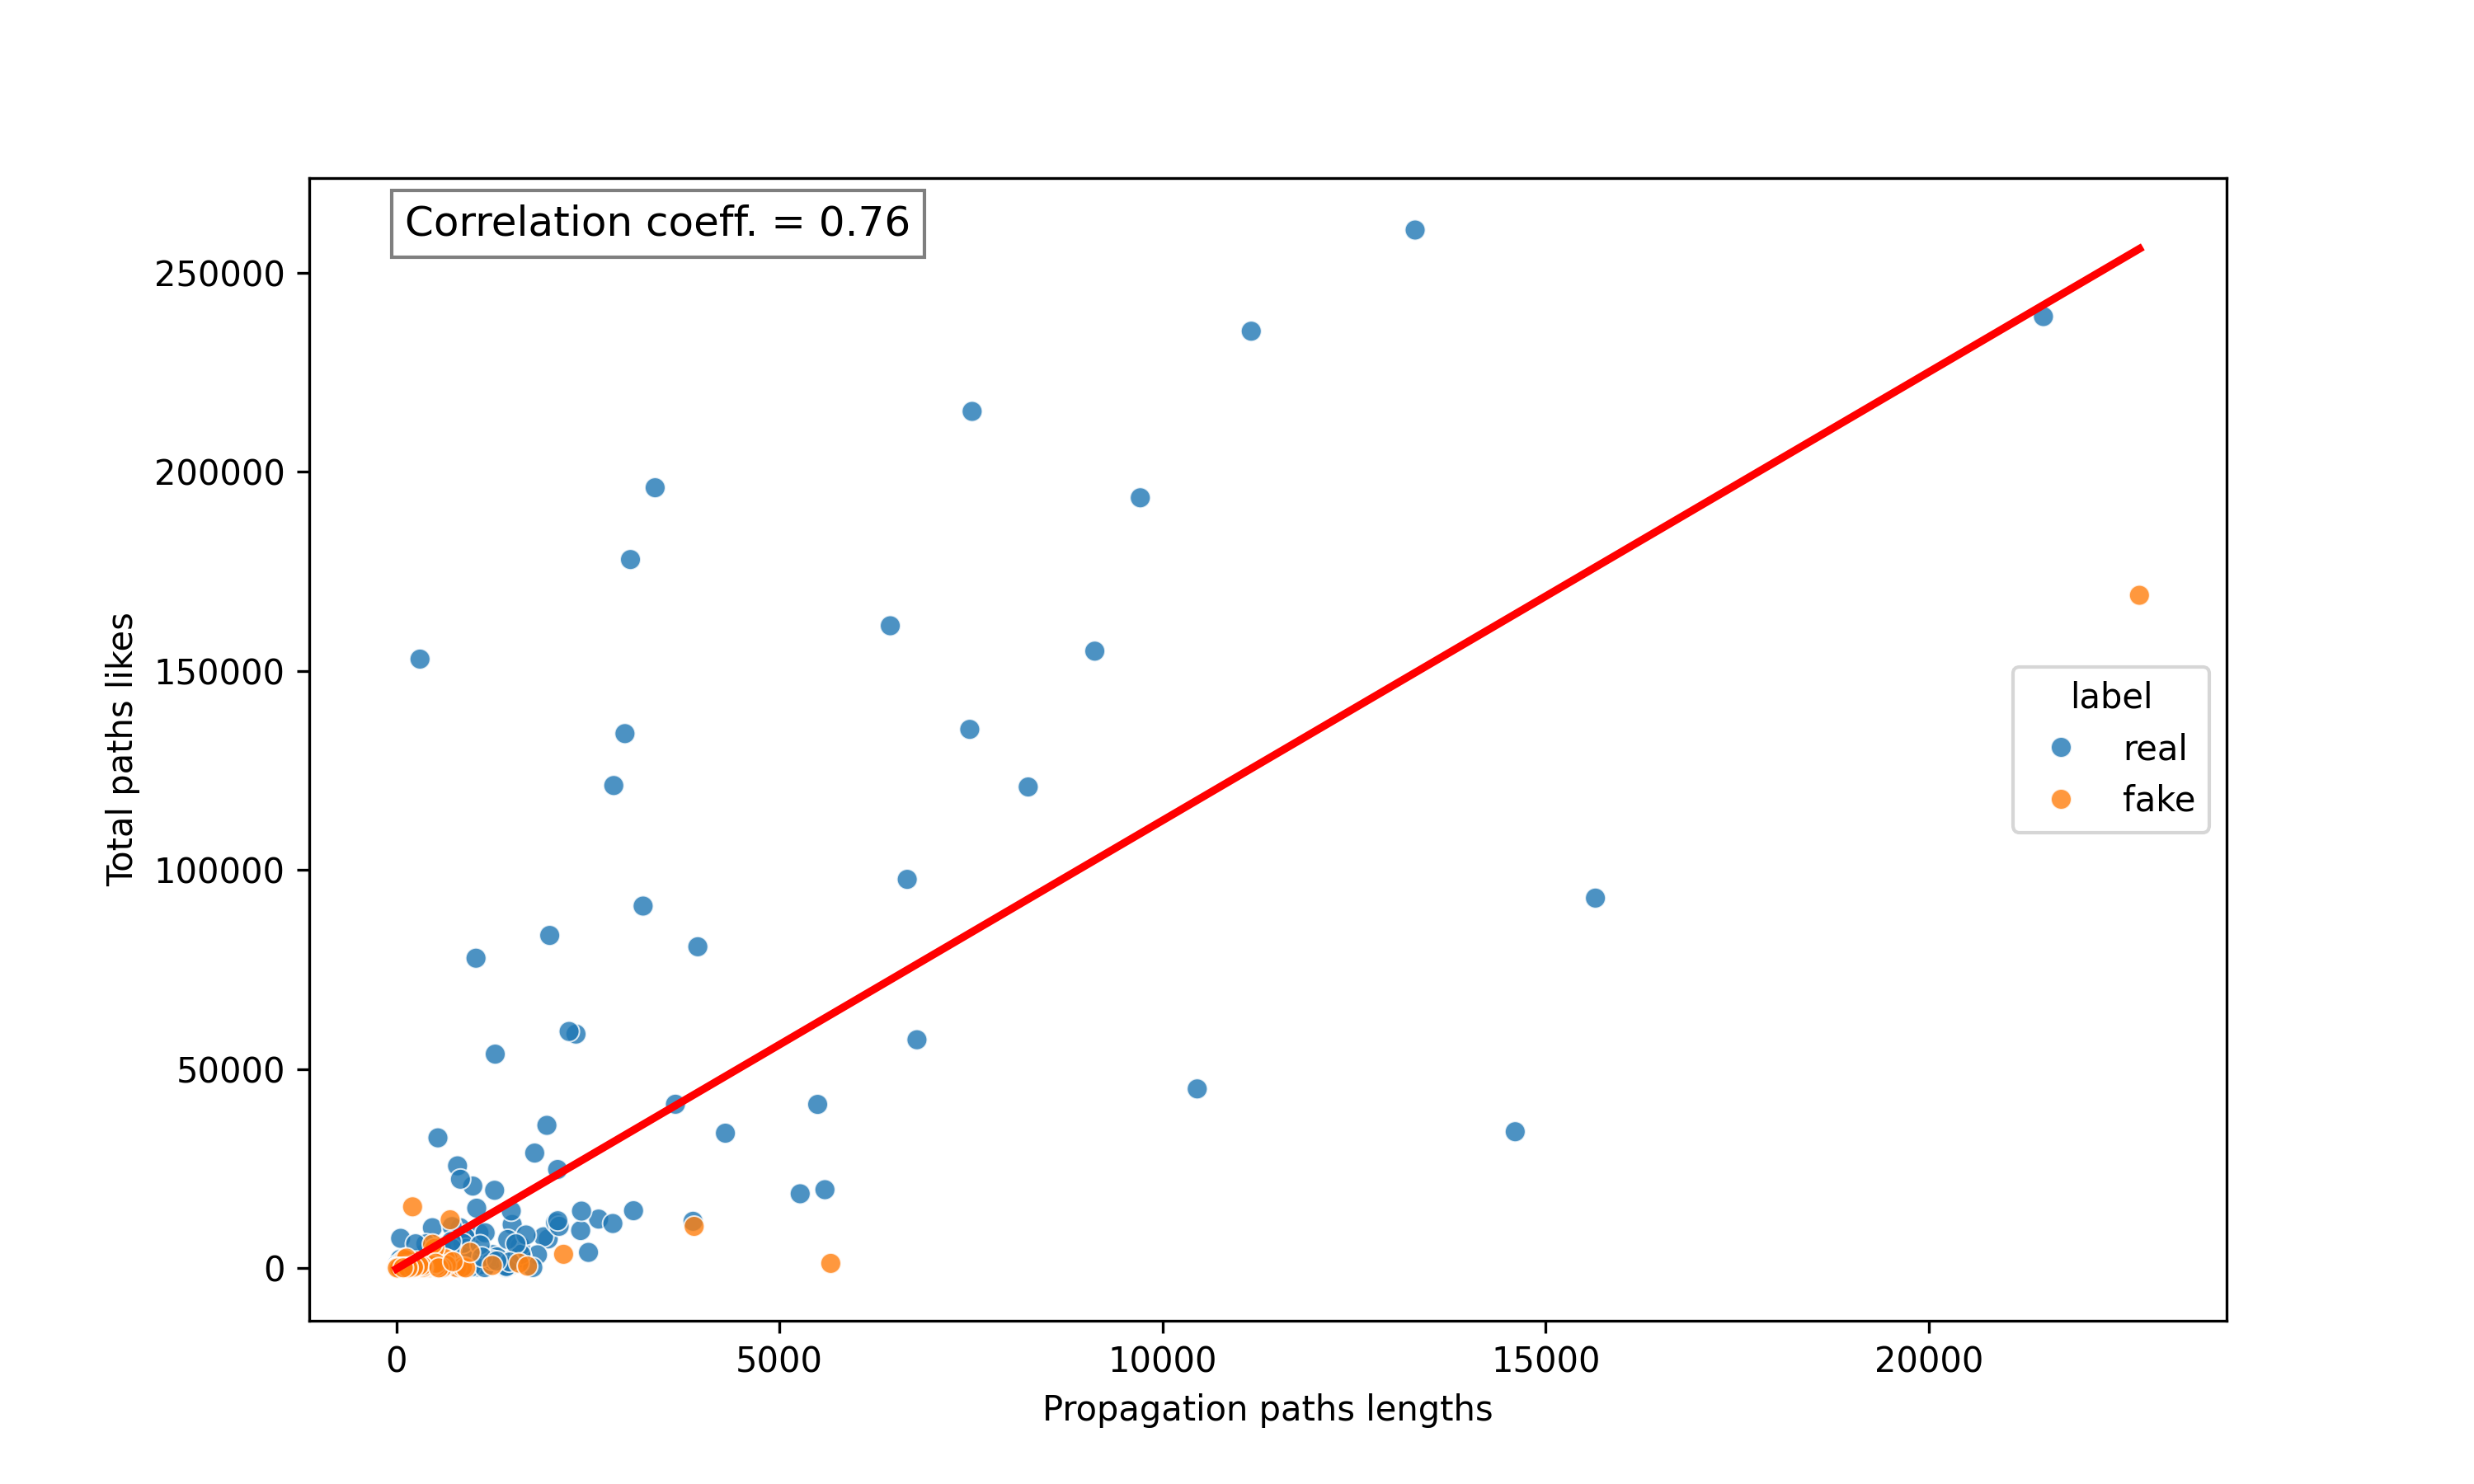
\includegraphics[width=\textwidth]{./img/scatter_plot_with_regression_colored.png}
	\caption{Total paths likes vs. propagation path lengths}
	\label{fig:corr_likes_len}
\end{figure}

Another preprocessing step involved transforming the total number of likes $L_i$ of each propagation path into a binary classification label, analogous to the approach used for the Evons dataset. However, due to the relatively small number of data points ($N < 600$), we could not adopt the exact same thresholding criteria used in that case, otherwise the viral class would be too underrepresented.

Instead, a median-based thresholding strategy was chosen: we computed the median $m_L$ of the distribution $\{ L_1, L_2, \dots, L_N \}$, and labeled each series $S_i$ as viral if $L_i > m_L$, and non-viral otherwise. Formally, the binary label $v_i$ assigned to series $S_i$ is defined as:

$$
v_i =
\begin{cases}
	1 & \text{if } L_i > m_L \\
	0 & \text{otherwise}
\end{cases}
$$

This transformation results in a perfectly balanced binary classification dataset, with an equal number of viral and non-viral instances. However, this methodological choice also constitutes a limitation of the study: as shown in Table ~\ref{tab:stats_likes_paths}, the median values for both resulting groups are relatively low in absolute terms. \\

The final preprocessing step concerns the standardization of the length of tweet series. Since the sequences $S_i$ vary in length ($n_i = |S_i|$), we transformed them to a fixed length $\ell$ (the choice criteria of $\ell$ actual value will be treated in the third chapter)

For each series $S_i$:

\begin{itemize}
	\item If $n_i > \ell$, the sequence was truncated to its first $\ell$ tweets.
	\item If $n_i < \ell$, the sequence was padded with synthetic tweets containing zero-valued features, so that $|S_i| = \ell$ for all $i \in \{1, \dots, N\}$.
\end{itemize}

Formally, the resulting standardized sequences can be denoted as:

$$
S_i^{(\ell)} = \{ T_{i1}, T_{i2}, \dots, T_{i\ell} \}
$$

Each tweet $T_{ij}$ retains all original features as previously defined. Unlike the procedure adopted for the Evons dataset, in this case the number of likes per tweet ($\text{likes}_{ij}$) is included among the input features for classification. This is justified by the nature of the task, which involves prediction on longer time series. Consequently, the inclusion of this variable does not introduce data leakage, as the goal is to model the dynamics of propagation after observing tweet interactions over time.

\vspace{2em}

\begin{figure}[h!]
	\centering
	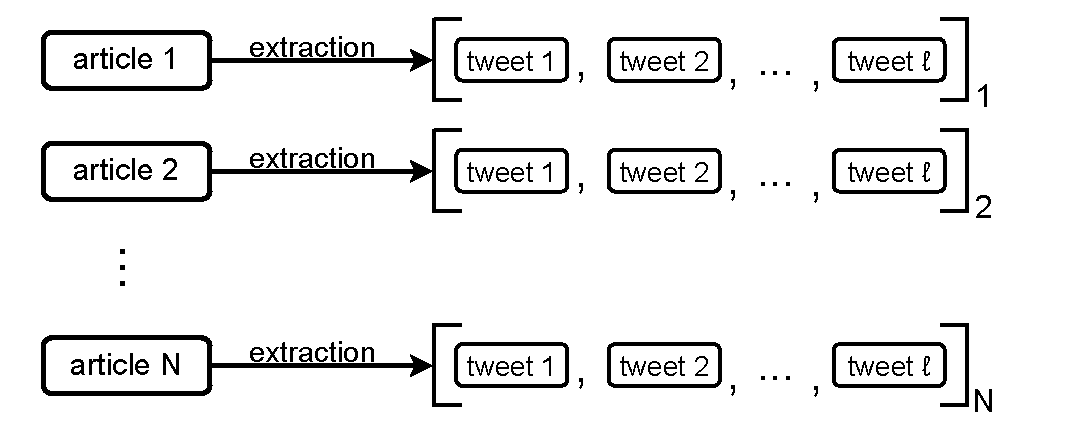
\includegraphics[width=\textwidth]{./img/article_tweet_diagram-2.pdf}
	\caption{Schematization of tweets extraction from articles. $\ell$ is a fixed length}
	\label{fig:articles_to_series}
\end{figure}

\chapter{Methods} \label{Methods}
This chapter illustrates the methods used in this work. The structure will be as follows. First, we will analyze the methods used on the Evons dataset. As for the order of prediction tasks, we will follow the interpretative grid in page \pageref{tab:grid}: first fake news detection, then virality prediction.
Next, we will move on to the FakeNewsDetection dataset, following the same order for prediction tasks.

\section{Evons methods}
In this section, we analyze the methods used on the Evons dataset.

\subsection*{Fake news detection}
\addcontentsline{toc}{subsection}{Fake news detection}

\subsubsection*{Input data}
\addcontentsline{toc}{subsubsection}{Input data}

As explained in the previous section, the data we have is a series of articles: $\mathcal{A} = \{ a_1, a_2, \dots, a_N \}$ with $N = 92{,}969$. Each article $a_i$ is associated with a tuple of features. That is,
\[
a_i = (t_i, c_i, s_i, e_i), \quad \text{for } i = 1, \dots, N.
\]

The components of each tuple are defined as follows:
\begin{itemize}
	\item $t_i$: the title of article $i$,
	\item $c_i$: the Facebook caption accompanying article $i$,
	\item $s_i$: the source of article $i$,
	\item $e_i$: the number of Facebook engagements for article $i$.
\end{itemize}


For each article $i$, there is an associated label $y_i$ indicating whether the article is true or false. 
Since the goal of this task is to identify false articles, the label is defined as:
$$
y_i =
\begin{cases}
	1 & \text{if the article is fake} \\
	0 & \text{if the article is true}
\end{cases}
$$

As described in section \ref{evons_pres}, the truth or falsehood of the articles was determined by the dataset curators based on the source of origin. Consequently, we removed the source $s_i$ and the number of Facebook engagements $e_i$ from the features of each article $a_i$. At this point, therefore, each article corresponds to $a_i = (t_i, c_i)$, that is, a tuple containing the title and the Facebook caption. \\

To obtain vector representations of the title $t_i$ and caption $c_i$ of each article, we employed the \texttt{RoBERTa} model \footcite{liu2019}, a transformer-based language model developed by Facebook AI that improves upon BERT. 
Given a tokenized text input $x$, we passed it through the \texttt{RoBERTa} model and we extracted the hidden state corresponding to the \texttt{[CLS]} token (i.e., the first token in the sequence), which encodes the general meaning of the text. This process yields two separate embeddings for each article: one for the title, $\mathbf{d}^{(t)}_i \in \mathbb{R}^{768}$ , and one for the caption, $\mathbf{d}^{(c)}_i \in \mathbb{R}^{768}$. Both have length $l=768$. Each article can now be defined as a tuple containing both embeddings:

\[
a_i = (\mathbf{d}^{(t)}_i, \mathbf{d}^{(c)}_i), \quad \text{for } i = 1, \dots, N.
\]

This represents the final input data for the prediction model.

\subsubsection*{Problem definition and model description} \label{evons_detection}
\addcontentsline{toc}{subsubsection}{Problem definition and model description}

The task can be formalized as a binary text classification problem. 
Given an article $a_i$ represented by the pair of embeddings $(\mathbf{d}^{(t)}_i, \mathbf{d}^{(c)}_i)$, the goal is to predict the associated label $y_i \in \{0,1\}$, where $y_i = 1$ indicates a fake article and $y_i = 0$ indicates a true one.

\noindent Formally, we aim to learn a mapping:
\[
f: (\mathbf{d}^{(t)}, \mathbf{d}^{(c)}) \mapsto y
\]
that can accurately classify unseen articles based solely on their title and caption embeddings. To do this, we use a simple classification model based on a concatenation and a multilayer perceptron with a single output. The model takes as input the title embedding $\mathbf{d}^{(t)} \in \mathbb{R}^{768}$ and the caption embedding $\mathbf{d}^{(c)} \in \mathbb{R}^{768}$.  
These vectors are concatenated to form
\[
\mathbf{x} = \mathrm{concat}(\mathbf{d}^{(t)}, \mathbf{d}^{(c)}) \in \mathbb{R}^{1536}.
\]
The first linear transformation projects $\mathbf{x}$ into a hidden representation of 512 dimensions:
\[
\mathbf{h}_1 = W_1 \mathbf{x} + \mathbf{b}_1, \quad W_1 \in \mathbb{R}^{512 \times 1536},\ \mathbf{b}_1 \in \mathbb{R}^{512}.
\]
The resulting hidden vector passes then through a normalization layer, producing vector $\mathbf{h}_2$, which is then passed through GELU activation function $\phi$, an alternative to the more common ReLU that has shown better performance in several cases\footcite{lee2023}, and through a dropout layer:
\[
\mathbf{h}_3 = \text{Dropout}(\phi(\mathbf{h}_2)
)
\]

Finally, a second linear layer maps the hidden representation to a single logit:
\[
z = W_2 \mathbf{h}_3 + b_2, \quad W_2 \in \mathbb{R}^{1 \times 512},\ b_2 \in \mathbb{R}.
\]

Given the ground truth label $y \in \{0,1\}$, the model parameters are optimized using the binary cross-entropy loss with logits, adjusted with a positive class weight $w_{\text{pos}} > 0$ to address class imbalance (which, in this case, is relatively small):
$$
\text{Loss}(z, y) = -\left[ w_{\text{pos}} \cdot y \log\sigma(z) + (1-y)\log(1-\sigma(z))\right],
$$

where $\sigma$ is the sigmoid function and $w_{\text{pos}}$ increases the penalty for misclassifying positive ($y=1$) samples. \\
Here below is a visual scheme of the model.

\begin{figure}[h!]
	\centering
	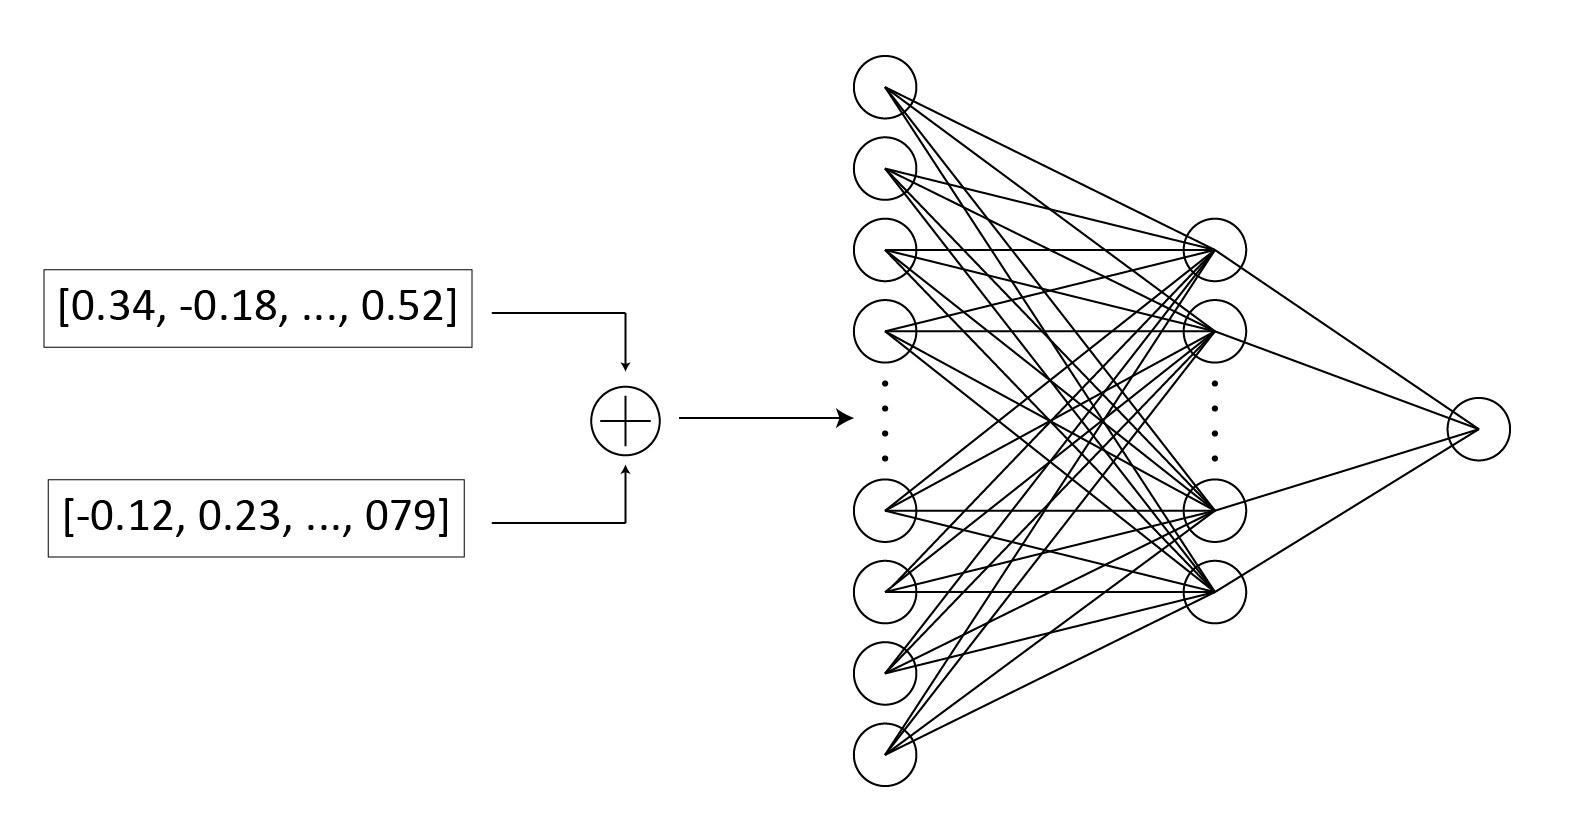
\includegraphics[width=0.8\textwidth]{./img/mlp_architecture.png}
	\caption{Embeddings concatenation with MLP head architecture}
	\label{fig:mlp_architecture}
\end{figure}

After manually searching for combinations of hyperparameters, those that guaranteed the best performance were selected. Since the primary focus of this work is to test different architectures, rather than different combinations of parameters, automatic hyperparameter optimization methods were not used. \\

As will be seen in the next chapter, the results of this model on the fake news detection task are virtually perfect and leave little room for improvement. For this reason, it was decided to proceed directly to the analysis of the more challenging task of predicting virality.

\subsection*{Virality prediction}
\addcontentsline{toc}{subsection}{Virality prediction}

\subsubsection*{Input data}
\addcontentsline{toc}{subsubsection}{Input data}
For this activity, the starting point is the same as in the previous section: a series of articles $\mathcal{A} = \{ a_1, a_2, \dots, a_N \}$ with $N = 92{,}969$, where each article $a_i$ is associated with a tuple of features $a_i = (t_i, c_i, s_i, e_i)$. \\

For each article $i$, there is an associated label $v_i$. The definition of the virality label was already shown on page \pageref{evons_processing}. We report it here as well for more clarity. Let $\tau$ denote the 95th percentile of the Facebook engagements distribution $\{ e_1, e_2, \dots, e_N \}$. Then:

$$
v_i = 
\begin{cases}
	1 & \text{if } e_i \geq \tau \quad \text{(viral)} \\
	0 & \text{otherwise} \quad \text{(non-viral)}
\end{cases}
$$  

The objective of the task is  to predict the virality of an article, regardless of its truth or falsehood. Consequently, $e_i$ is eliminated from the article tuples, as it is the value underlying the creation of the label $v_i$ itself. The source information, $s_i$, was not removed in advance. We tested various architectures, some of which used the source information as input and others that did not, to assess its contribution to prediction performance. \\
The textual elements of each article, $t_i$ and $c_i$, were transformed in two 768-dimensional BERT embeddings, $\mathbf{d}^{(t)}$ and $\mathbf{d}^{(c)}$ respectively, in the exact same way as before, using the \texttt{RoBERTa} model.

\subsubsection*{Problem definition}
\addcontentsline{toc}{subsubsection}{Problem definition}

As before, this task can be formalized as a binary classification problem. That is, learning a mapping such as:

\[
f: (a) \mapsto v
\]

To do this, we tried a different range of approaches and models. Before moving on to the analysis of the different architectures, however, it is worth dwelling on another aspect. Regardless of the type of model used, the main problem concerns data imbalance. The viral class makes up only 5\% of the dataset. This is a classic difficulty in machine learning: when faced with underrepresented classes, models struggle to learn and generalize. \\
There are three main possible solutions. The first two are oversampling and undersampling, which involve modifying the training data. In oversampling, the entries in the most represented class are multiplied to achieve greater balance. In undersampling, on the other hand, balance is achieved by eliminating entries from the most represented class. Finally, the third solution consists of using weighted loss functions during training, so as to give more importance to errors in the least represented class.\\

In an early research phase, we experimented with all three strategies. For oversampling, we used the \texttt{nlpaug} library\footcite{ma2019nlpaug}, which allows us to create multiple similar versions of the same source text by replacing certain words with synonyms, using a masked language modeling strategy based on BERT models. 	\\
After several preliminary tests, we found that models performances with oversampling or undersampling was equal to or worse than with a weighted loss alone. Therefore, we chose to use only the weighted loss approach for the rest of the research.

\subsubsection*{Model 1: MLP}
\addcontentsline{toc}{subsubsection}{Model 1: MLP}

The first model consists of the exact same architecture used in the Fake News Detection task on page \pageref{evons_detection}, so a multilayer perceptron that takes as input the concatenation of $\mathbf{d}^{(t)}$ and $\mathbf{d}^{(c)}$ and has a single logit as output.

\subsubsection*{Model 2: source embedding}
\addcontentsline{toc}{subsubsection}{Model 2: source embedding}

The second model extends the previous multilayer perceptron by incorporating an additional discrete source indicator into the input. Let $s \in \{0, \dots, S-1\}$ be an integer index representing the source of the news item, where $S$ is the total number of sources (here $S = 11$).

First, the textual embeddings are projected into a lower-dimensional space via learned linear transformations:
\[
\mathbf{h}^{(t)} = \phi\left(W_t \mathbf{d}^{(t)} + \mathbf{b}_t \right) \in \mathbb{R}^{192}, \quad
\mathbf{h}^{(c)} = \phi\left(W_c \mathbf{d}^{(c)} + \mathbf{b}_c \right) \in \mathbb{R}^{192},
\]
where $W_t, W_c \in \mathbb{R}^{192\times 768}$, $\mathbf{b}_t, \mathbf{b}_c \in \mathbb{R}^{192}$, and $\phi$ denotes, as before, the GELU activation function.

The source index $s$ is mapped to a dense embedding vector via a learned embedding matrix $E \in \mathbb{R}^{S\times 192}$:
\[
\mathbf{h}^{(s)} = \phi\left(E_{s:}\right) \in \mathbb{R}^{192}.
\]

The three representations are concatenated to form a single feature vector:
\[
\mathbf{h}_3 = \text{concat}(\mathbf{h}^{(t)}, \mathbf{h}^{(c)}, \mathbf{h}^{(s)}) \in \mathbb{R}^{576}.
\]

Finally, a linear classifier produces a scalar logit:
\[
z = W_h \mathbf{h}_3 + b,
\]
with $W_h \in \mathbb{R}^{1 \times 576}$ and $b \in \mathbb{R}$. The model is trained using a weighted binary cross-entropy loss with logits. Here below is a visual scheme of the model's architecture.

While this architecture can include information about an article’s source, it has a major limitation: once the model is trained on a specific dataset, it cannot process sources not present in the training data. For example, if the total number of sources is $S = 11$ (as it is in our case), the model cannot handle a case where $s = 12$ if that value was not seen during training. 

\vspace{1em}

\begin{figure}[h!]
	\centering
	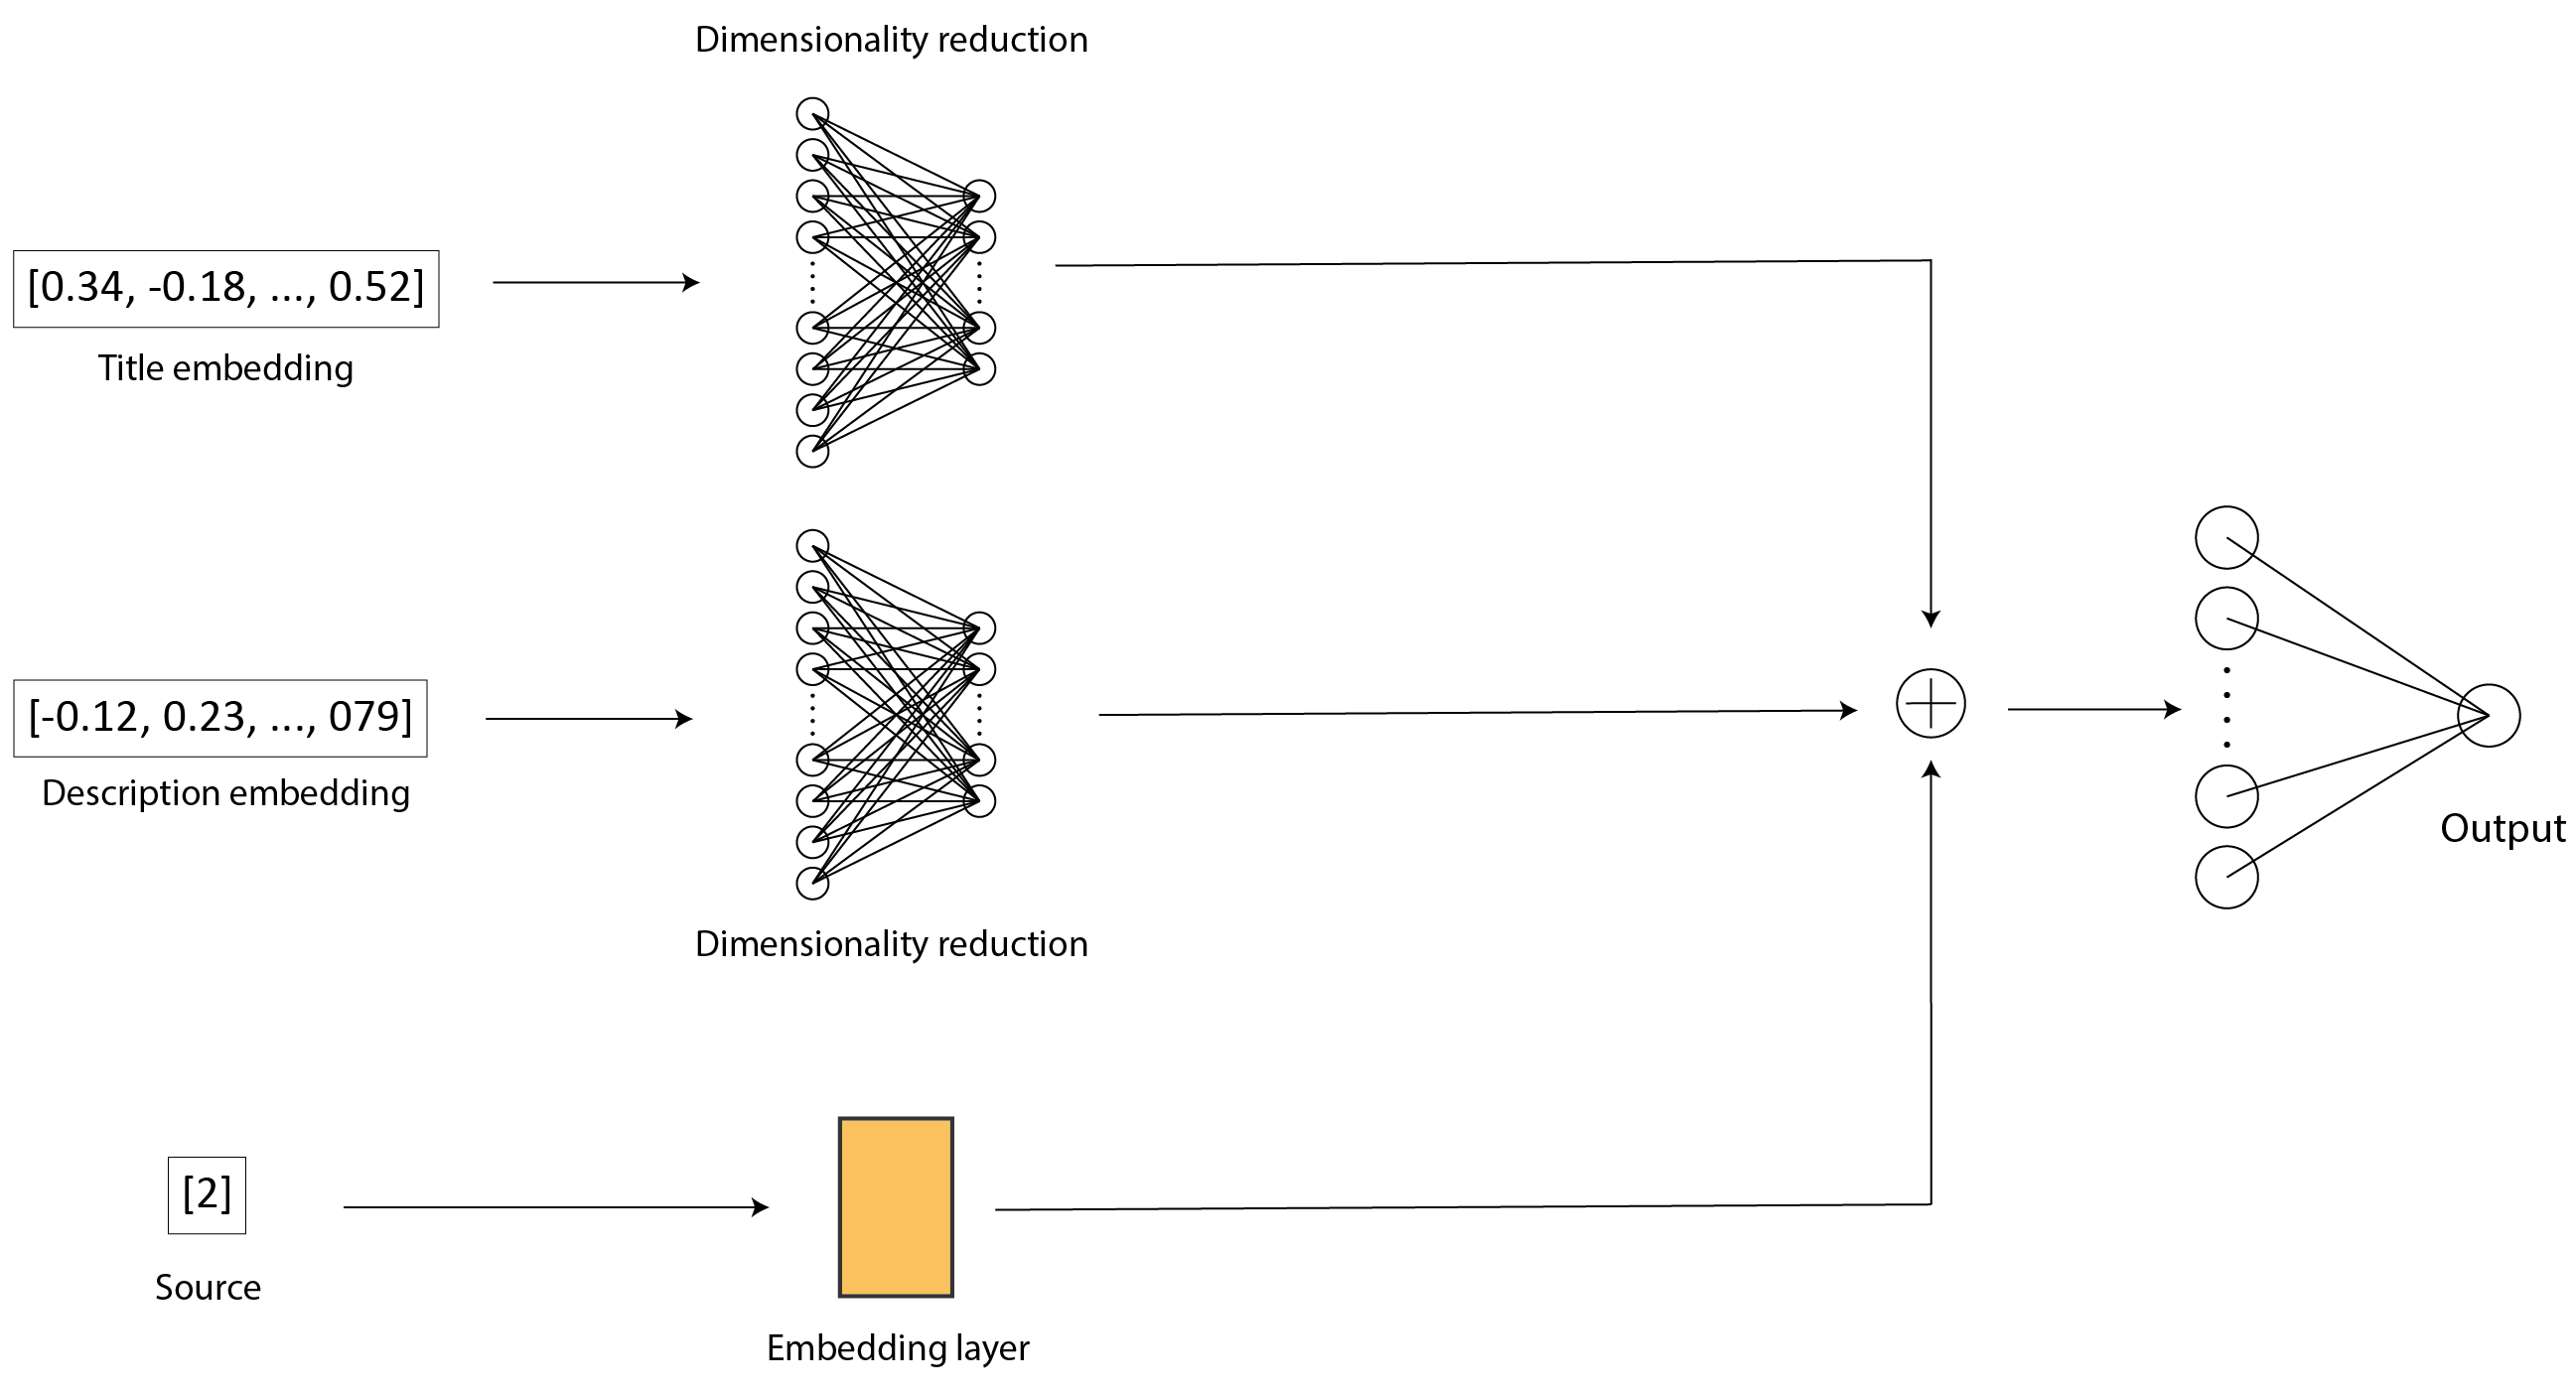
\includegraphics[width=1.1\textwidth]{./img/2_mlp_architecture.png}
	\caption{Text embeddings reduction with source embedding architecture}
\end{figure}

\clearpage

\subsubsection*{Model 3: average engagement feature} \label{model 3}
\addcontentsline{toc}{subsubsection}{Model 3: average engagement feature}

To overcome the limitation of the previous model, which was unable to handle sources not seen during training, the third model uses a different approach. It replaces the discrete source embedding of the previous architecture with a continuous source-level feature derived from engagement statistics.  
For each source in the training data, we compute from the mean number of Facebook engagements for that source. Then, instead of using directly the source index as input data for the model, we use the average number of Facebook engagements. Formally, for each source $s$ appearing in the training data we define:
\[
g_s = \frac{1}{n_s} \sum_{i:\, s(i) = s} e_i,
\]
where $e_i$ is the number of engagements for article $i$, $n_s$ is the number of training articles from source $s$, and $s(i)$ denotes the source of article $i$.  
To mitigate skew, the average engagement is log-transformed and standardized using the mean and variance from the training set, as explained mathematically below:

\begin{enumerate}
	\item Log transform:
	\[
	\tilde{g}_s = \log\left(1 + g_s\right)
	\]
	\item Standardization:
	\[
	\hat{g}_s = \frac{\tilde{g}_s - \mu_{\text{train}}}{\sigma_{\text{train}}},
	\]
	where $\mu_{\text{train}}$ and $\sigma_{\text{train}}$ are the mean and standard deviation of $\tilde{g}_s$ across all sources in the training set.
\end{enumerate}

The model processes three inputs: the title embedding $\mathbf{d}^{(t)} \in \mathbb{R}^{768}$, the content embedding $\mathbf{d}^{(c)} \in \mathbb{R}^{768}$, and the scalar engagement feature $g_s$.

As in the previous model, the textual embeddings are projected into a lower-dimensional space via learned linear transformations:
\[
\mathbf{h}^{(t)} = \phi\left(W_t \mathbf{d}^{(t)} + \mathbf{b}_t \right) \in \mathbb{R}^{192}, \quad
\mathbf{h}^{(c)} = \phi\left(W_c \mathbf{d}^{(c)} + \mathbf{b}_c \right) \in \mathbb{R}^{192},
\]
where $\phi$ is the GELU activation function,  $W_t, W_c \in \mathbb{R}^{192\times 768}$ and $\mathbf{b}_t, \mathbf{b}_c \in \mathbb{R}^{192}$.

The scalar engagement feature is also projected into the same space via a learned linear transformation:
\[
\mathbf{h}^{(g)} = \phi\left(W_g \, g_s + \mathbf{b}_g \right) \in \mathbb{R}^{192},
\]
where $W_g \in \mathbb{R}^{192 \times 1}$ and $\mathbf{b}_g \in \mathbb{R}^{192}$.

The three representations are concatenated to form:
\[
\mathbf{h}_3 = \text{concat}(\mathbf{h}^{(t)}, \mathbf{h}^{(c)}, \mathbf{h}^{(g)}) \in \mathbb{R}^{576}.
\]

Finally, a linear classifier produces a scalar logit:
\[
z = W_h \mathbf{h}_3 + b,
\]
with $W_h\in \mathbb{R}^{1 \times 576}$ and $b \in \mathbb{R}$.

The model is trained using the binary cross-entropy loss with logits, weighted to account for class imbalance. \\

This architecture allows for a more flexible handling of sources. In the case of real applications of such a model, in fact, the average number of engagements for a certain source can easily be calculated by scraping the last $n$ posts from that source. As a result, the model can handle any source, even one never seen in the training data, as long as the average number of engagements is available for that source. 
Here below is a visualization of the model. 

\begin{figure}[h!]
	\centering
	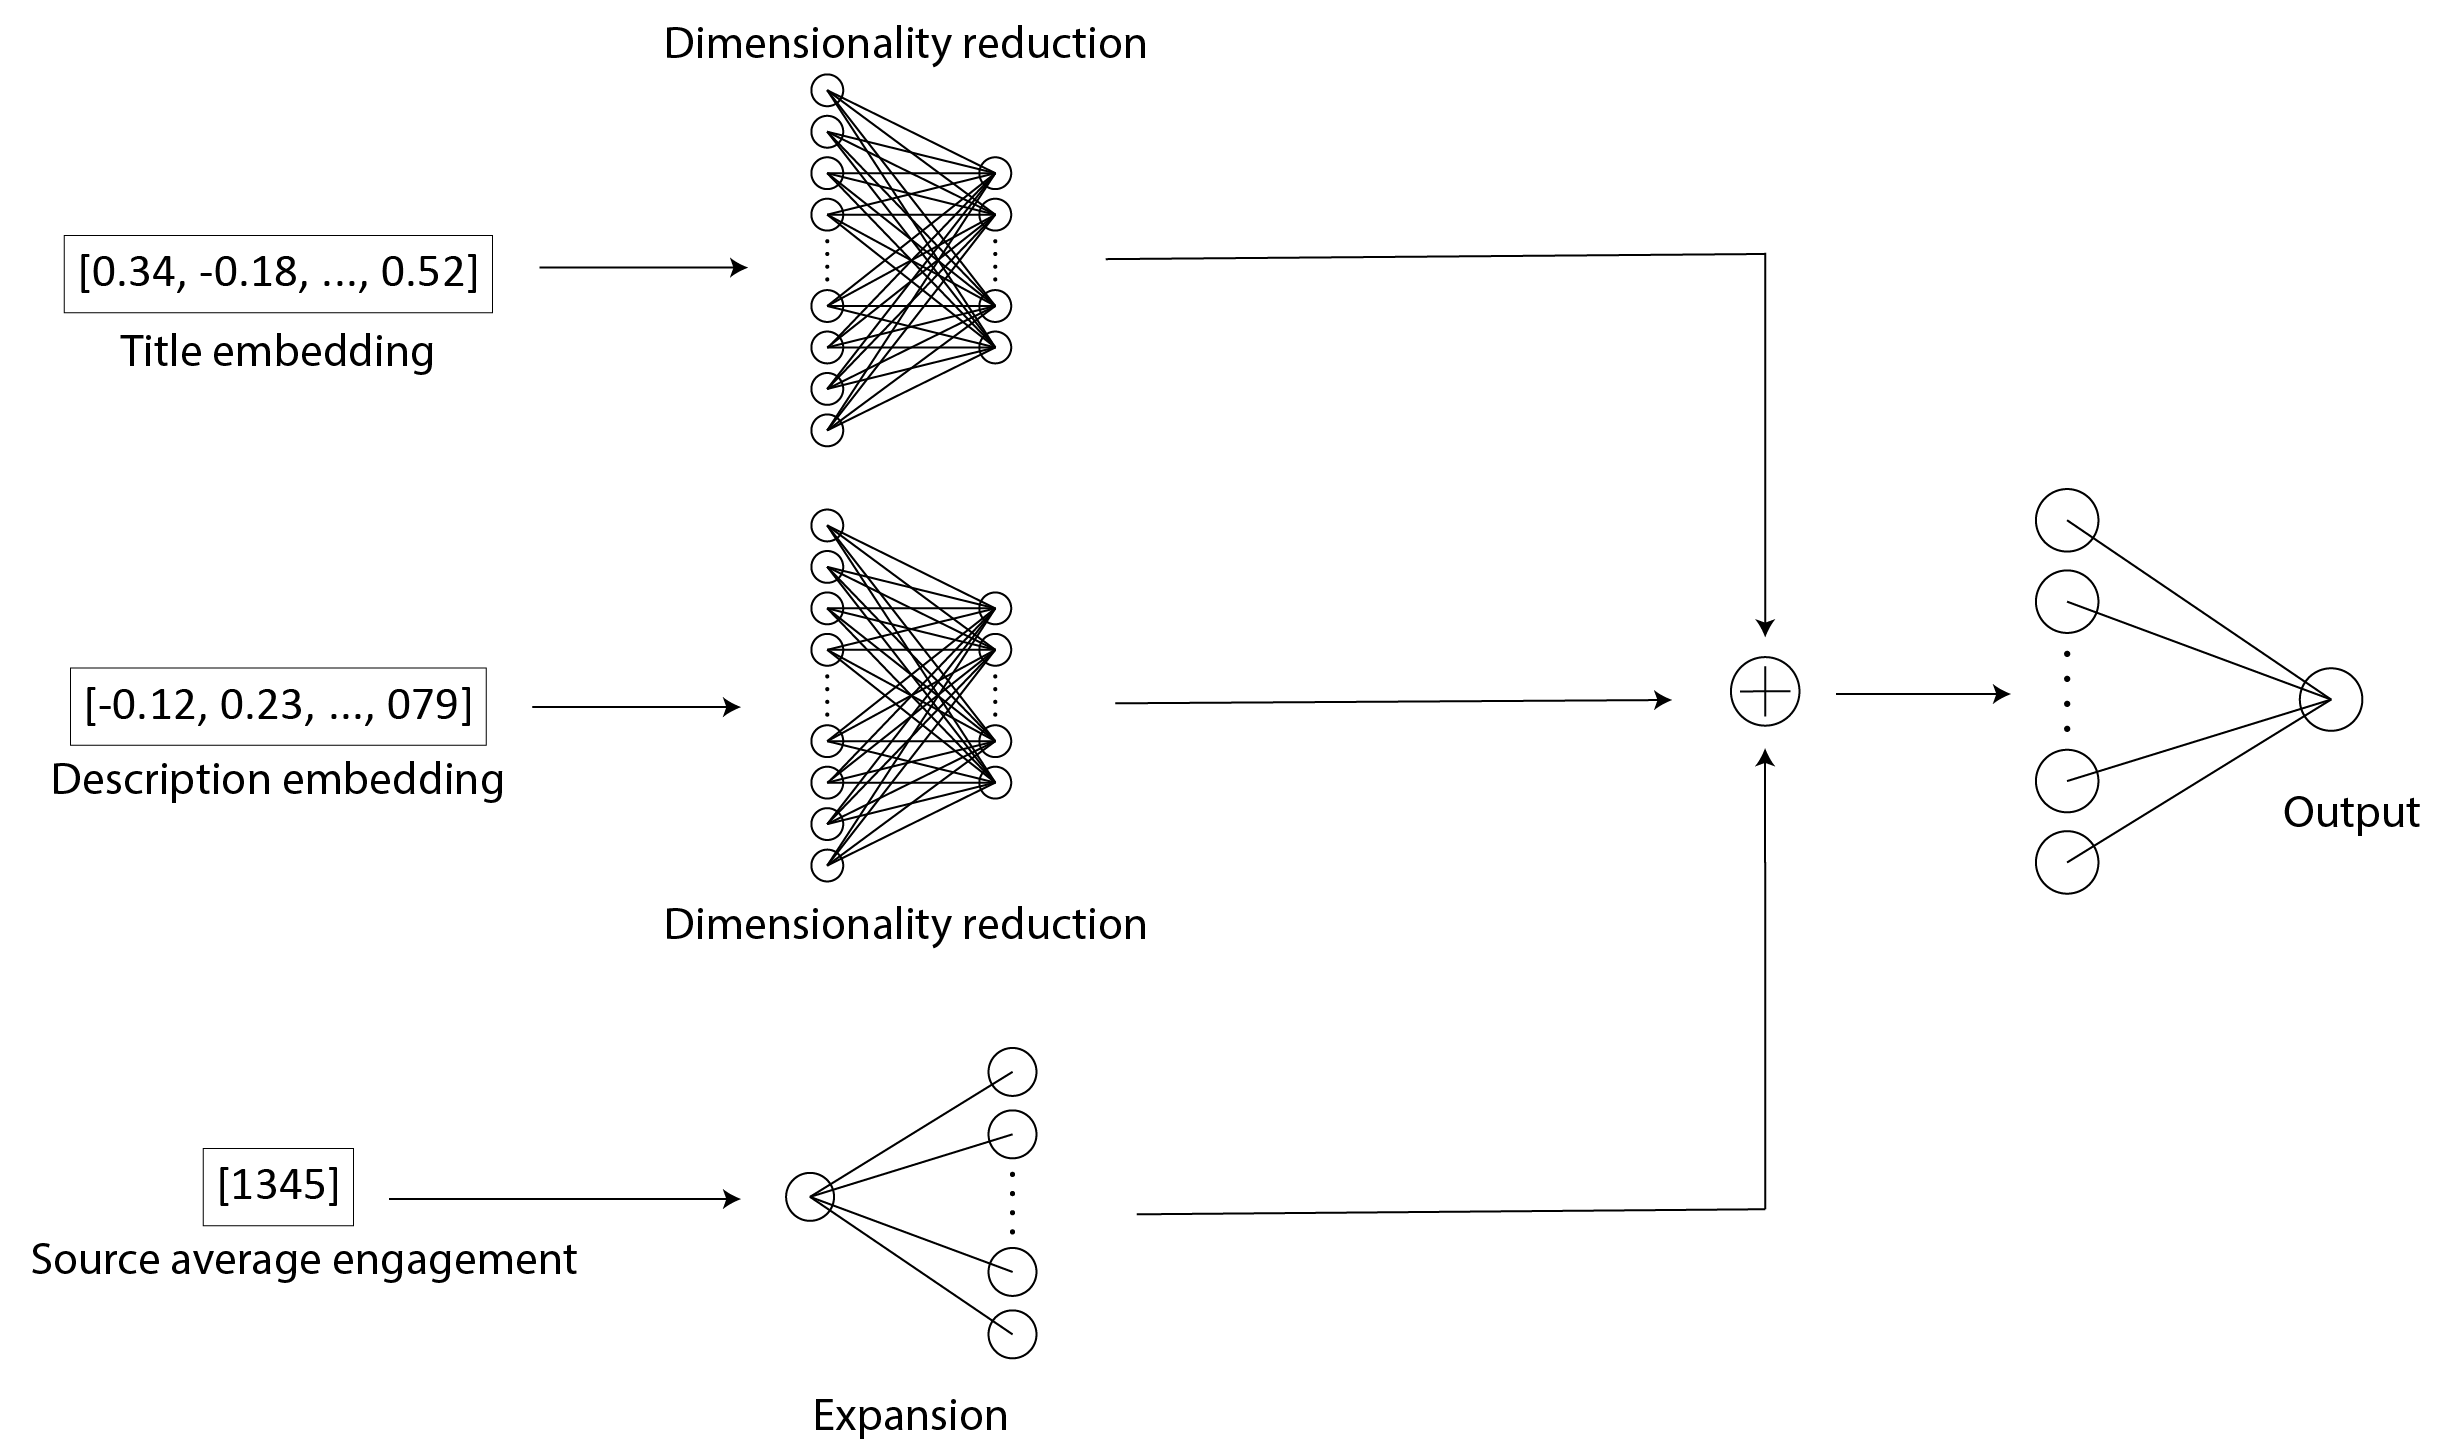
\includegraphics[width=1.1\textwidth]{./img/3_mlp_architecture.png}
	\caption{Text embeddings reduction with average engagement per source embedding}
\end{figure}

\subsubsection*{Model 4: gated fusion of text and engagement}
\addcontentsline{toc}{subsubsection}{Model 4: gated fusion of text and engagement}

This model extends the previous approach by replacing plain concatenation with a learned, per-dimension \emph{gating} mechanism that blends textual information with the continuous engagement feature. The inputs are the same as in Model 3: the title embedding $\mathbf{d}^{(t)} \in \mathbb{R}^{768}$, the content embedding $\mathbf{d}^{(c)} \in \mathbb{R}^{768}$, and the (log-transformed and standardized) source-level engagement scalar $g_s \in \mathbb{R}$.

As before, textual embeddings are projected into a lower-dimensional space using learned linear maps followed by a GELU activation:
\[
\mathbf{h}^{(t)} = \phi\left(W_t \mathbf{d}^{(t)} + \mathbf{b}_t \right) \in \mathbb{R}^{192}, \quad
\mathbf{h}^{(c)} = \phi\left(W_c \mathbf{d}^{(c)} + \mathbf{b}_c \right) \in \mathbb{R}^{192},
\]
where $\phi$ is the GELU activation function,  $W_t, W_c \in \mathbb{R}^{192\times 768}$ and $\mathbf{b}_t, \mathbf{b}_c \in \mathbb{R}^{192}$. The two are then concatenated to obtain the textual representation
\[
\mathbf{h}^{(\text{text})} \;=\; \text{concat}(\mathbf{h}^{(t)}, \mathbf{h}^{(c)}) \in \mathbb{R}^{384}.
\]

The engagement scalar is mapped into the same space via a learned linear transformation and GELU:
\[
\mathbf{h}^{(e)} \;=\; \phi(W_e \, g_s + \mathbf{b}_e) \in \mathbb{R}^{384},
\]
where $W_e \in \mathbb{R}^{384 \times 1}$ and $\mathbf{b}_e \in \mathbb{R}^{384}$.

To fuse the two branches, the model computes a data-dependent gate $\mathbf{p}\in\mathbb{R}^{384}$ by applying a sigmoid to an affine transformation of the concatenated pair, so that each value of the resulting vector is between 0 and 1:
\[
\mathbf{p} \;=\; \sigma\!\big(W_{\text{gate}} \,\text{concat}(\mathbf{h}^{(\text{text})}, \mathbf{h}^{(e)}) + \mathbf{b}_{\text{gate}}\big) \in \mathbb{R}^{384},
\]
with $W_{\text{gate}} \in \mathbb{R}^{384 \times 768}$ and $\mathbf{b}_{\text{gate}} \in \mathbb{R}^{384}$. The gate is then used to assign corresponding weights to each dimension of $\mathbf{h}^{\text{(text)}}$ and $\mathbf{h}^{\text{(e)}}$, following prior research\footcite{arevalo2017}:
\[
\mathbf{b} \;=\; \mathbf{p} \odot \mathbf{h}^{(\text{text})} \;+\; (1-\mathbf{p}) \odot \mathbf{h}^{(e)} \in \mathbb{R}^{384},
\]
where $\odot$ is the Hadamard product (e.g. an element-wise multiplication). The blended vector passes then through a GELU activation and a linear classifier that outputs a single scalar:

\[
z \;=\; W_z \phi(\mathbf{b}) + b_z, \qquad
W_z \in \mathbb{R}^{1 \times 384},\;\; b_z \in \mathbb{R}.
\]
The model is trained using the binary cross-entropy loss with logits, weighted to account for class imbalance. \\

In this architecture, the gate $\mathbf{g}$ learns, for each feature dimension, how much to rely on textual evidence versus the engagement-derived features. In particular, for coordinate $j$ the fused value is $b_j = p_j h^{(\text{text})}_j + (1-p_j) h^{(e)}_j$; thus $p_j\!\approx\!1$ lets text dominate, while $g_j\!\approx\!0$ lets the engagement feature dominate. This mechanism allows the model to adaptively exploit the continuous source information while remaining robust to sources not observed during training. At the same time, such an architecture requires that the scalar feature of the average number of engagements for a source, $g_s$, be expanded to a number of dimensions equal to $\text{concat}(\mathbf{h}^{(\text{text})}, \mathbf{h}^{(\text{e})})$, which could excessively increase the number of weights in the model.
A visual representation of the model is shown below. 

These were the models tested in this study for the identification of viral publications for Evons dataset. The results will be presented in the following chapter. 

\begin{figure}[h!]
	\centering
	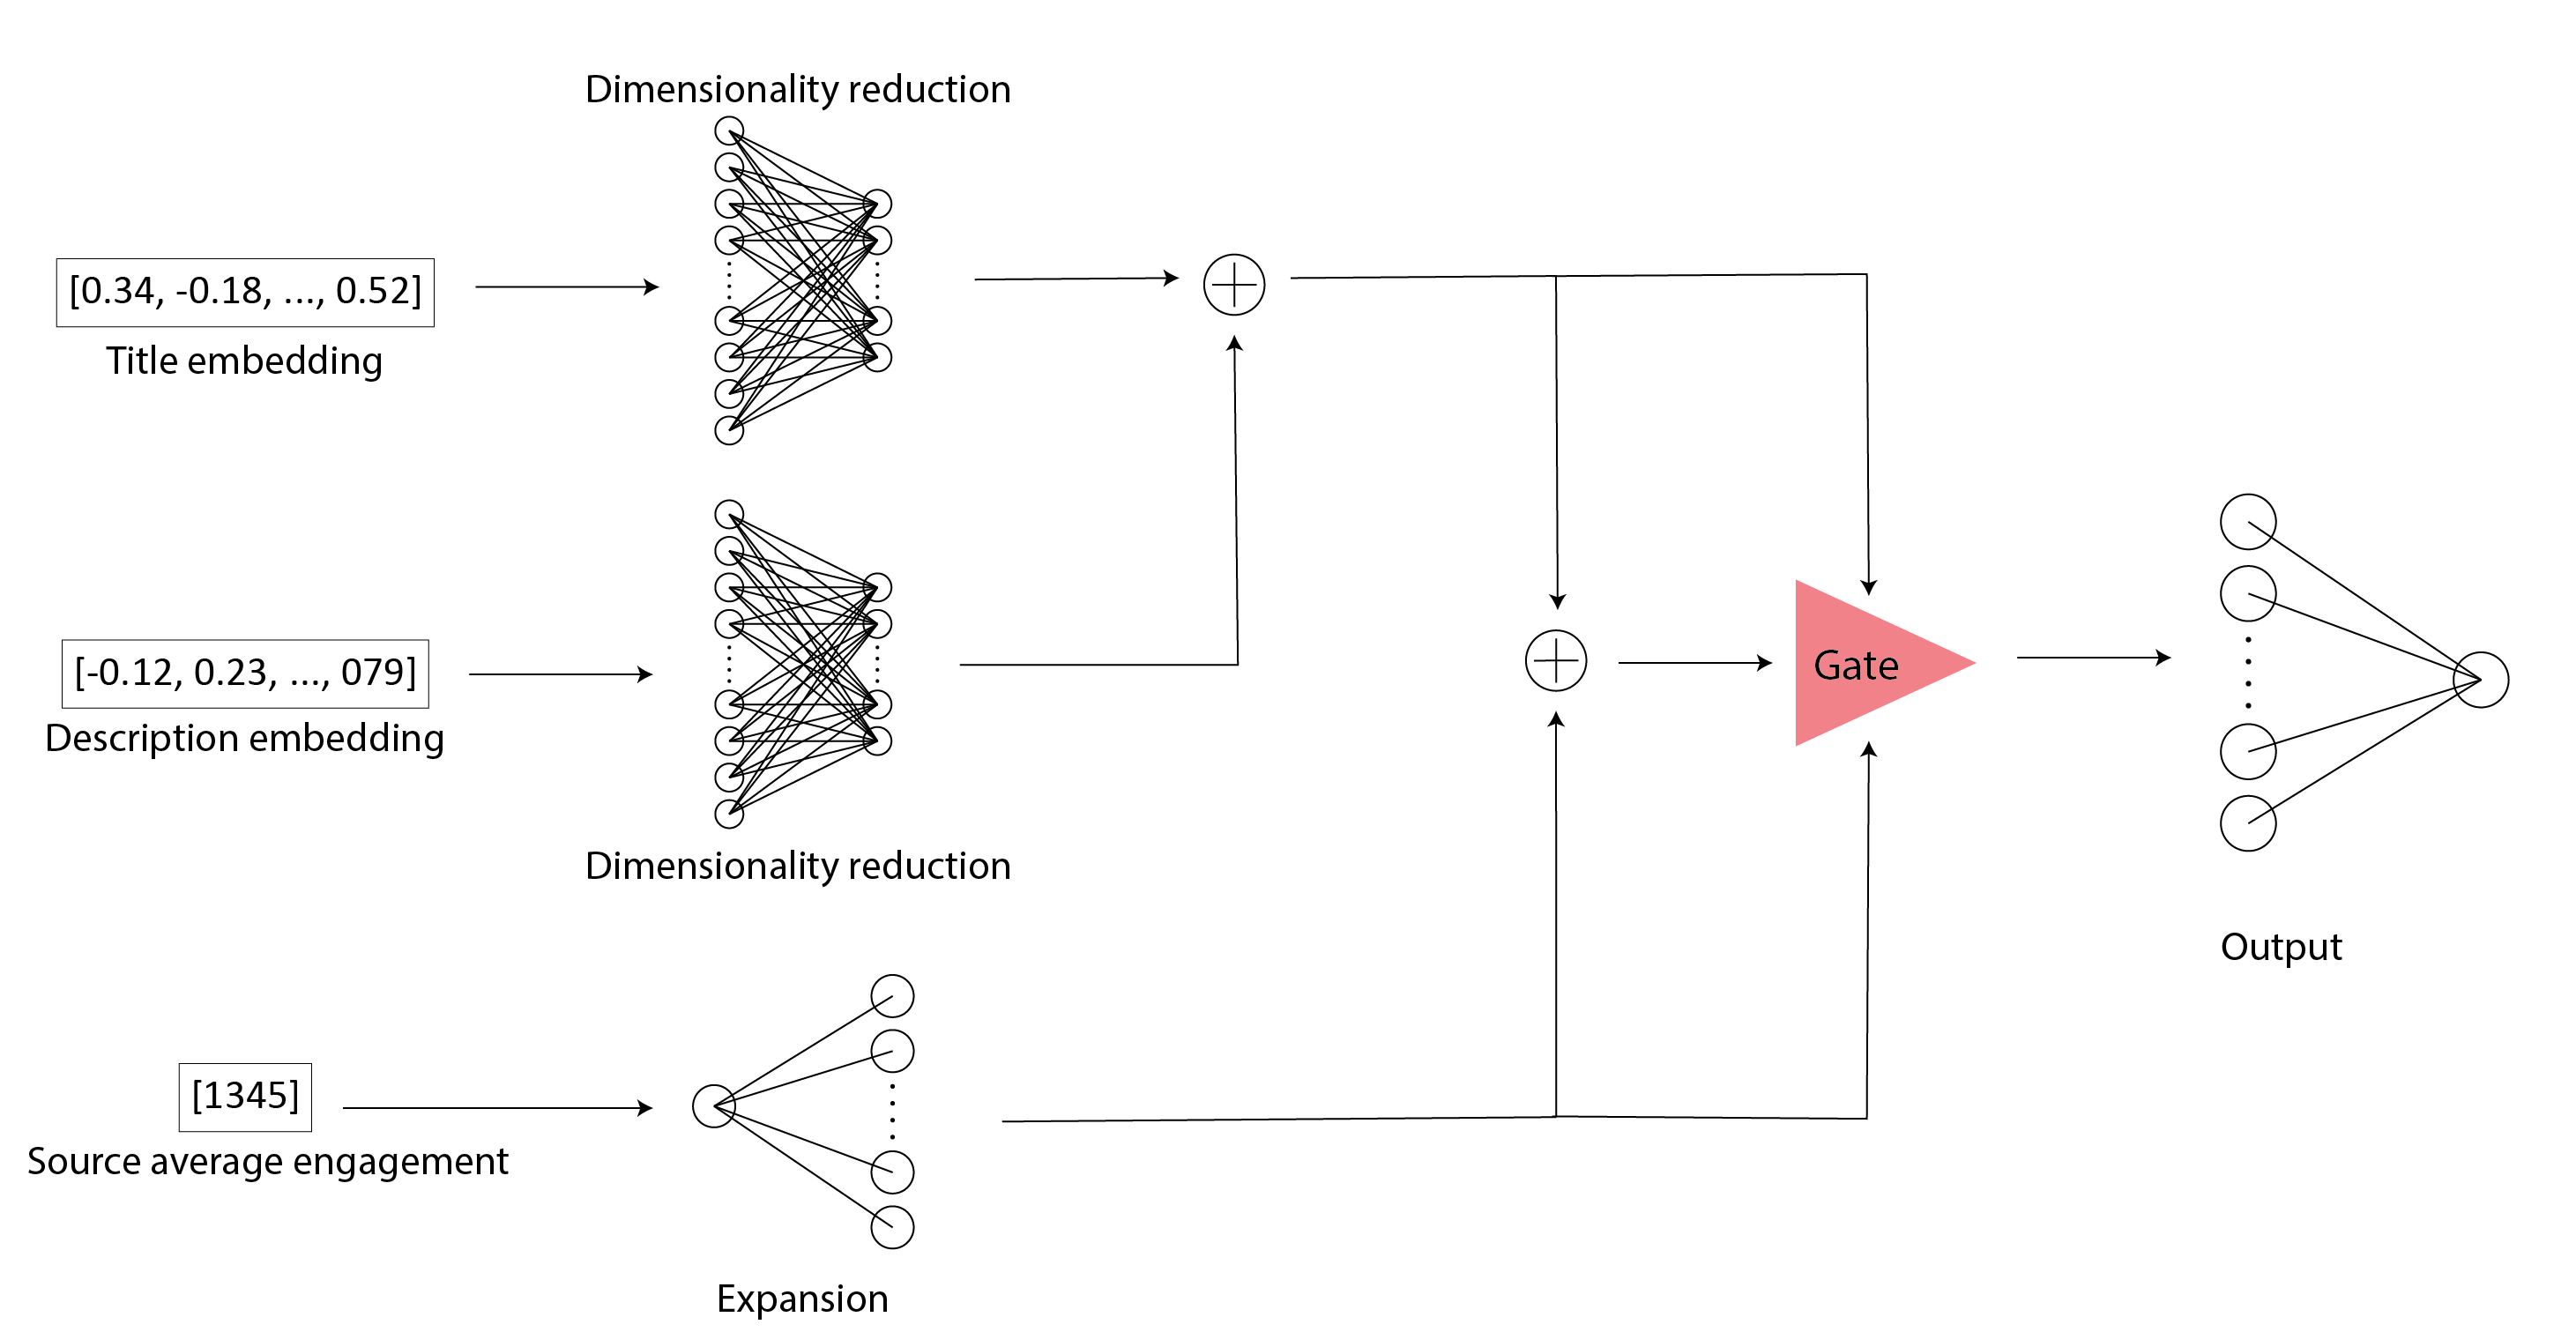
\includegraphics[width=1.1\textwidth]{./img/4_mlp_architecture.png}
	\caption{Gate fusioning of text and average engagement per source embeddings}
\end{figure}

\pagebreak

\section{FakeNewsNet methods}
In this section, we analyze the methods used on the FakeNewsNet dataset.

\subsection{Fake news detection} \label{fakenewsdata_detection_models}
\subsubsection*{Input data}
\addcontentsline{toc}{subsubsection}{Input data}

As already explained, our starting point is a collection $\mathcal{T} = \{ S_1, S_2, \dots, S_N \}$ of propagation paths, where each $S_i$ represents a sequence of tweets associated with a given news article, in a chronological order. In total, we constructed $N = 578$ tweet series. Each series has a fixed length $\ell$, obtained through padding or truncation.
Each tweet $T_{ij} \in S_i$ is: 

$$
T_{ij} = \left( \text{text}_{ij},\ \Delta t_{ij},\ \text{followers}_{ij},\ \text{following}_{ij},\ \text{verified}_{ij},\ \text{likes}_{ij} \right)
$$

Each element is defined as follows:
\begin{itemize}
	\item $\text{text}_{ij}$ : text of tweet $ij$
	\item $\Delta t_{ij}$ : difference from publication times of tweet $ij$ and the first tweet in the series $T_{i1}$
	\item $\text{followers}_{ij}$ : number of followers of tweet author's account
	\item $\text{following}_{ij}$ : number of following of tweet author's account
	\item $\text{verified}_{ij}$ : binary variable indicating if tweet author's account is verified
	\item $\text{likes}_{ij}$ : likes obtained by tweet $ij$
\end{itemize}

For each series $S_i$, we also have a binary label $y_i$ defined as follows:

$$
y_i =
\begin{cases}
	1 & \text{if the article associated to } S_i \text{ is fake} \\
	0 & \text{if the article associated to } S_i \text{ is true}
\end{cases}
$$

For each tweet $T_{ij}$, we transformed the text in a 768-dimensions embedding $\mathbf{d}_{ij}$ using \texttt{RoBERTa}, as before. Non-binary numeric features (that is, every feature except $\text{text}_{ij}$ and  $\text{verified}_{ij}$) are log-transformed and standardized with the same procedure mentioned on page \pageref{model 3}: let $z_{ij}^{(k)}$ denote any non-binary numeric feature. The preprocessing is performed as follows:

\begin{enumerate}
	\item \textbf{Log transform}:
	\[
	\tilde{z}_{ij}^{(k)} = \log\left(1 + z_{ij}^{(k)}\right)
	\]
	
	\item \textbf{Standardization}:
	\[
	\hat{z}_{ij}^{(k)} = \frac{\tilde{z}_{ij}^{(k)} - \mu^{(k)}_{\text{train}}}{\sigma^{(k)}_{\text{train}}},
	\]
	where $\mu^{(k)}_{\text{train}}$ and $\sigma^{(k)}_{\text{train}}$ are the mean and standard deviation of $\tilde{z}_{ij}^{(k)}$ computed across all tweets in the training fold.
\end{enumerate}

\subsubsection{Problem definition}
\addcontentsline{toc}{subsubsection}{Problem definition}
This problem, like the previous ones, can be defined as a binary classification. In other words, we need to find a function that takes as input a tweet series $S_i$ and capable of mapping: 

\[
f: (S) \mapsto y
\]

Compared to the work on the Evons dataset, the main difference in this case lies in the data format. The $f$ function takes a series of data as input -- in other words, a series of vectors -- rather than a single vector. This sequential structure carries important temporal and relational information: the order of tweets, the time intervals between them, and the evolution of engagement metrics can all contribute to detecting whether a news article is fake or real. Consequently, the classification task must be approached with models capable of processing sequential data.

\subsubsection*{Model 1-2-3: bidirectional GRU, RNN, LSTM}
\addcontentsline{toc}{subsubsection}{Model 1-2-3: bidirectional GRU, RNN, LSTM}

The model then takes a series of tweets $S_i$ as input. For each tweet $T_{ij}$, the following operations are performed. Each tweet corresponds to a vector of 768 dimensions plus 5 numerical features. The 5 features are extracted from each tweet, creating a vector that we will call $\mathbf{n}_{ij} \in \mathbb{R}^5$. The resulting vector is then expanded through a linear layer to a 32 dimensions space: 

\[
\mathbf{e}_{ij} =  \phi\!\left(W_{\text{num}}\,\mathbf{n}_{ij} + \mathbf{b}_{\text{num}}\right)
\]
where $W_{\text{num}} \in \mathbb{R}^{32 \times 5}$, $\mathbf{b}_{\text{num}} \in \mathbb{R}^{32}$, and $\phi$ denotes the GELU function. The two vectors $\mathbf{d}_{ij}$ and $\mathbf{e}_{ij}$ are then concatenated to create a longer vector $\mathbf{x}_{ij} = \text{concat}(\mathbf{b}_{ij}, \mathbf{e}_{ij}) \in \mathbb{R}^{800}$. After applying this processing to all tweets of series $S_i$, we have an input sequence $(\mathbf{x}_{i1}, \dots, \mathbf{x}_{i\ell})$. This sequence is then processed by a bidirectional Gated Recurrent Unit model (GRU) with hidden size $H=128$ in each direction. At each position $j$, the GRU outputs the concatenated forward and backward hidden states:
\[
\mathbf{o}_{ij} = \text{concat}(\overrightarrow{\mathbf{h}}_{ij}, \overleftarrow{\mathbf{h}}_{ij}) \in \mathbb{R}^{256}
\]

From the GRU outputs, the representation at the last position $\mathbf{o}_{i\ell}$ is selected and fed into a two-layer feedforward classifier. 

The first layer maps $\mathbf{o}_{i\ell}$ to a 32-dimensional hidden vector with GELU activation:

\[
\mathbf{z}_i = \phi(W_1 \mathbf{o}_{i\ell} + \mathbf{b}_1)
\]

where $W_1 \in \mathbb{R}^{32 \times 256}$ and $\mathbf{b}_1 \in \mathbb{R}^{32}$. The second layer projects the resulting vector $\mathbf{z}_i \in \mathbb{R}^{32} $ to a scalar logit, followed by a sigmoid activation to produce the probability $\hat{y}_i$ of the article being fake:
\[
\hat{y}_i = \sigma(w^\top \mathbf{z}_i + b), \quad w \in \mathbb{R}^{32}, \ b \in \mathbb{R},
\]

The model is trained using the binary cross-entropy loss. A visual representation of the model is shown above. 

\begin{figure}
	\centering
	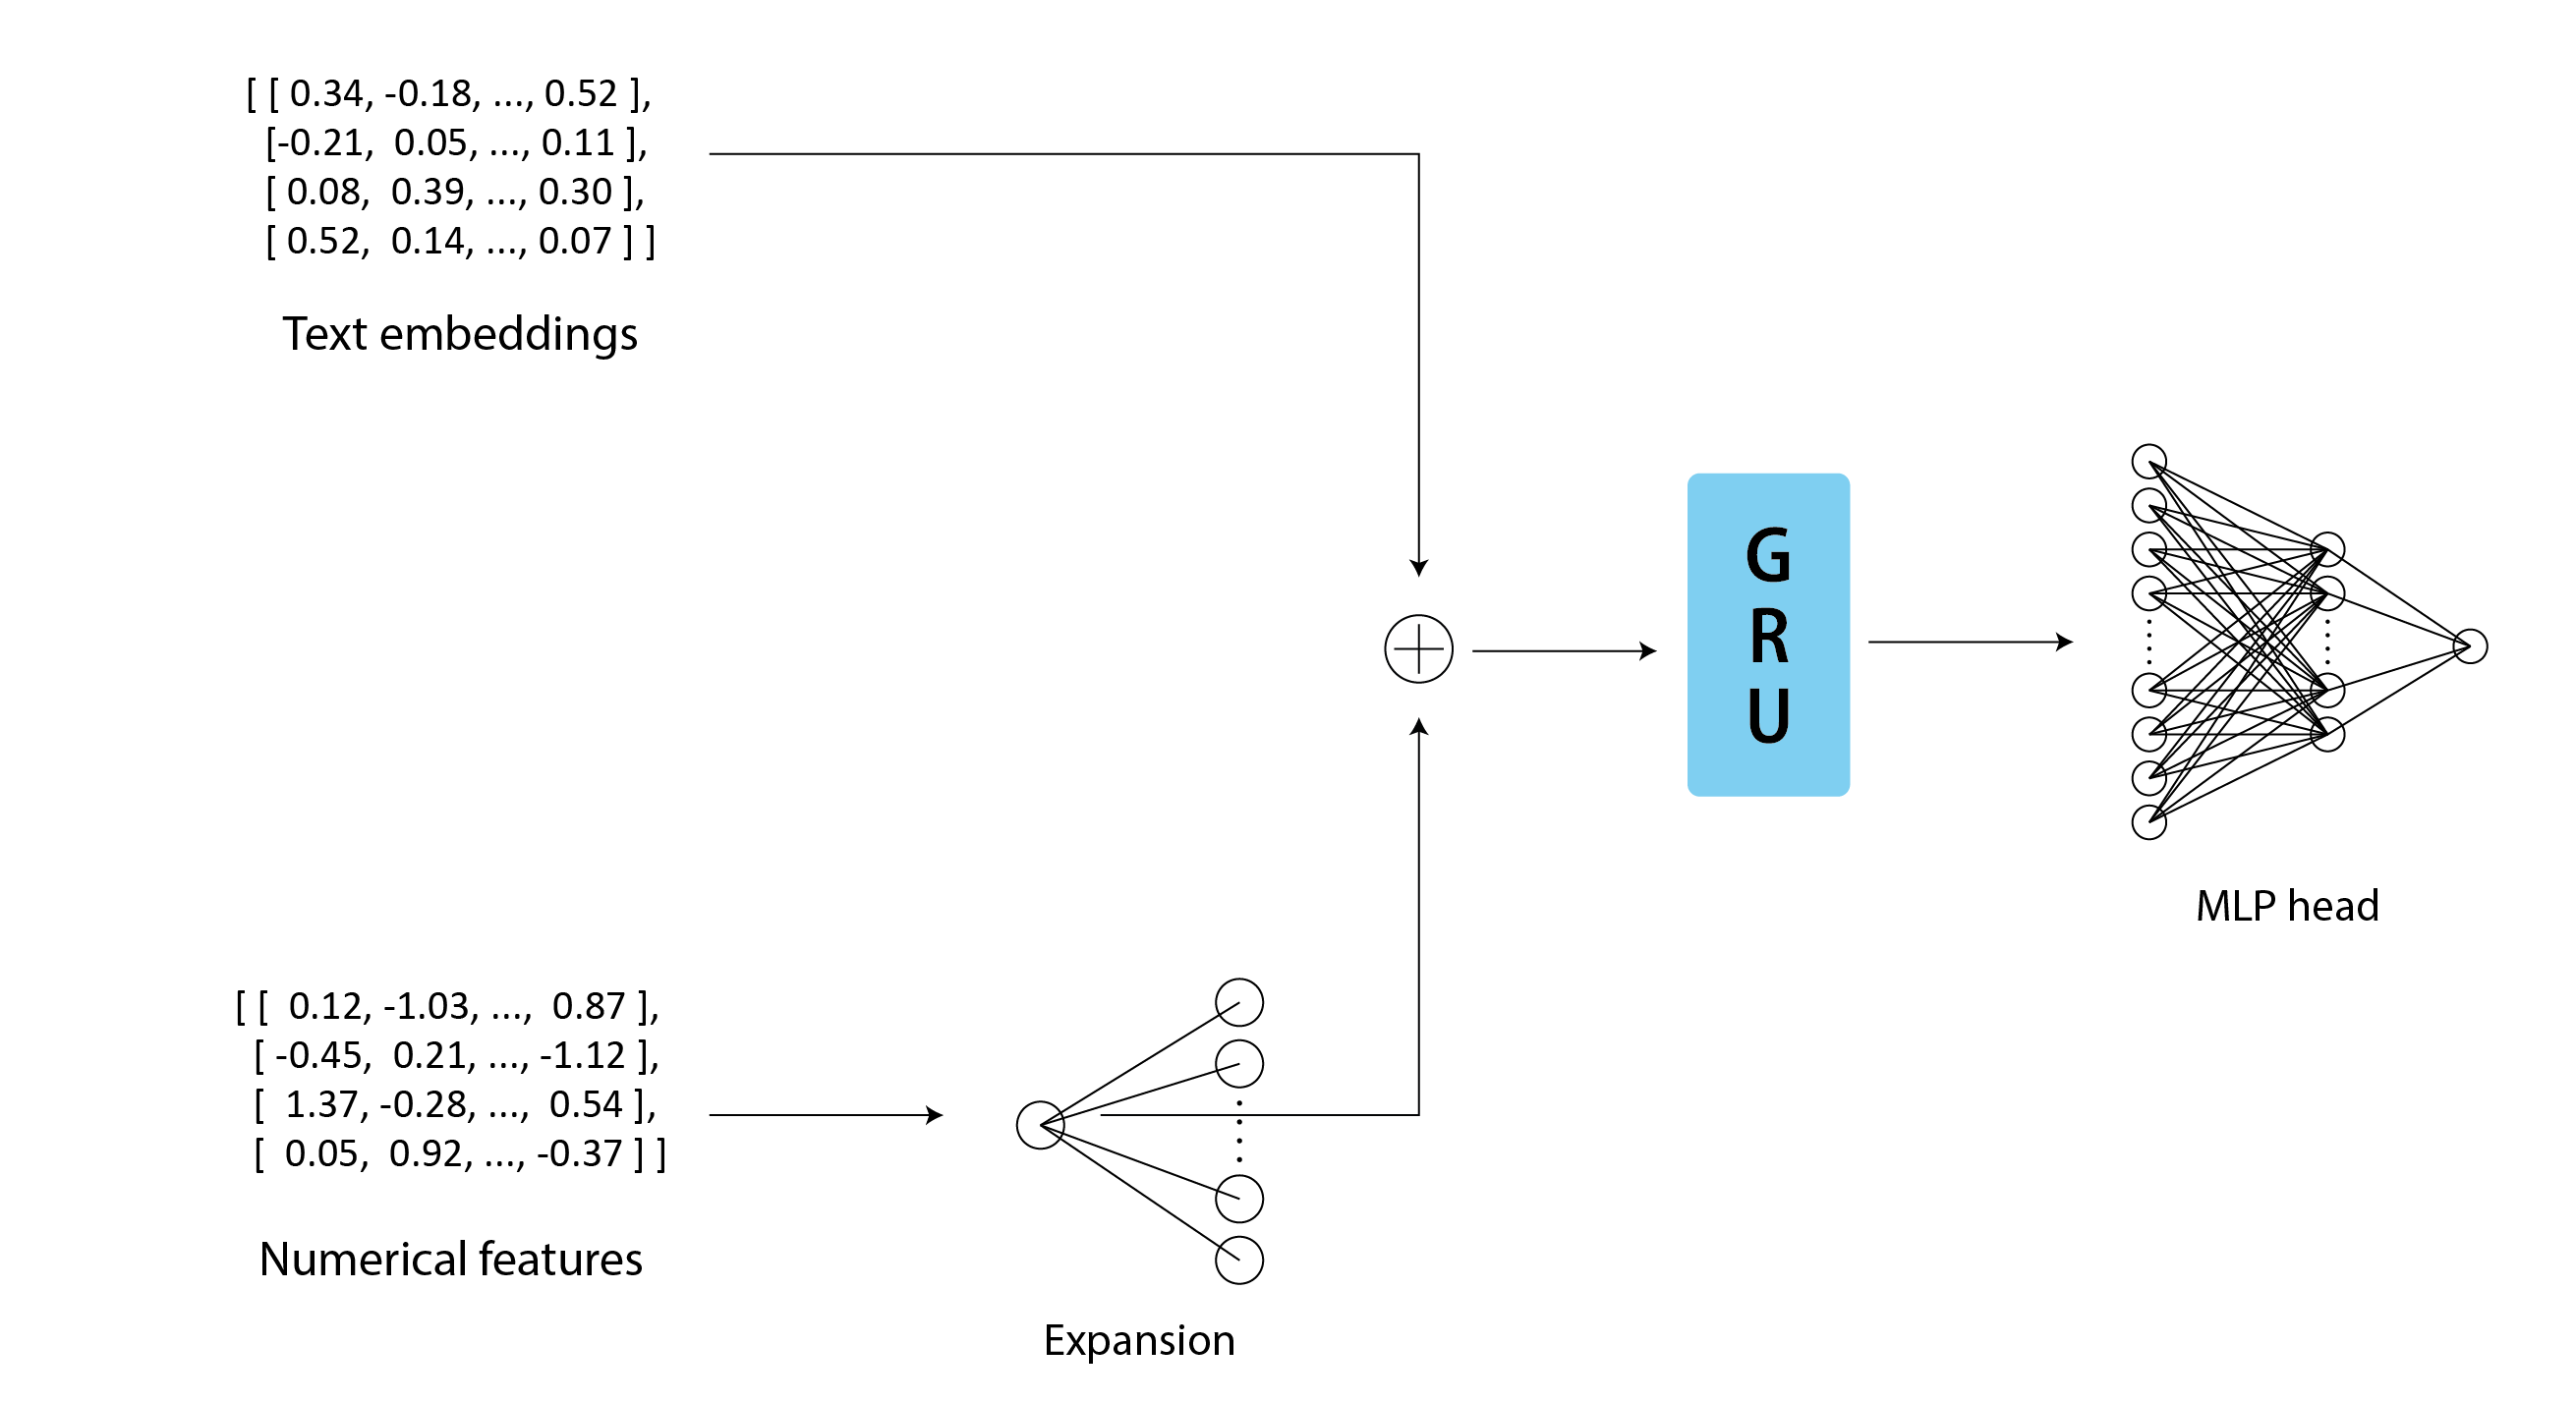
\includegraphics[width=1.1\textwidth]{./img/1_seq_model.png}
	\caption{Bidirectional GRU} \label{GRU}
\end{figure}


For two other models, we kept the same structure and changed only the recurrent part: GRU model was replaced with a long short-term memory model (LSTM) or with a plain recurrent neural network (RNN). Resulting in three different models tested. 

\subsubsection*{Model 4: convolutional neural network}
\addcontentsline{toc}{subsubsection}{Model 4: convolutional neural network}

This model is similar to the previous ones, with one major change: instead of RNN-based models as core mechanism, we use a convolutional neural network. As in the previous models, the first step consists in the projection of the five numeric features of each tweet $T_{ij}$ -- vector $\mathbf{n}_{ij}$ -- into a 32-dimensional space with a linear layer:
\[
\tilde{\mathbf{n}}_{ij}=\phi\!\left(W_n \mathbf{n}_{ij}+\mathbf{b}_n\right)\in\mathbb{R}^{32},\qquad
W_n\in\mathbb{R}^{32\times 5},\ \mathbf{b}_n\in\mathbb{R}^{32},
\]
and concatenated with the text embedding to form
\[
\mathbf{x}_{ij}=\text{concat}(\mathbf{d}_{ij},\ \tilde{\mathbf{n}}_{ij}), \quad \text{where } \mathbf{x}_{ij}\in\mathbb{R}^{800}
\]

After applying this processing to all tweets of series $S_i$, we have an input sequence $(\mathbf{x}_{i1}, \dots, \mathbf{x}_{i\ell})$. The data then passes through a block of two layers of convolutional neural networks to identify any local patterns useful for classification. For convolutions, which are performed only along the sequence length dimension, a window (kernel) of 3 elements, a padding equal to 1, and a 128-dimensional output were selected. Since the padding is equal to 1, CNN's output has an equal sequence length $\ell$ as the input.
Consequently:

\[
H^i = \text{CNN}((\mathbf{x}_{i1}, \dots, \mathbf{x}_{i\ell})) 
\]

where $H^{(i)} \in \mathbb{R}^{\ell\times128}$. The feature map $H^{(i)}$ is then reduced by a max pooling which, for each of the 128 output features, extracts the maximum value in the sequence. The resulting vector, then, is $\mathbf{h}_i \in \mathbb{R}^{128}$. \\
Finally, a two-layer perceptron maps $\mathbf{h_i}$ to a probability:
\[
\mathbf{u}_i=\phi(W_1\mathbf{h}_i+\mathbf{b}_1)\in\mathbb{R}^{32},\quad
\hat{y}_i=\sigma(\mathbf{w}_2^\top\mathbf{u}_i+b_2)
\]

The model is trained using a binary cross-entropy loss. A visual scheme of the model is presented above.

\begin{figure}
	\centering
	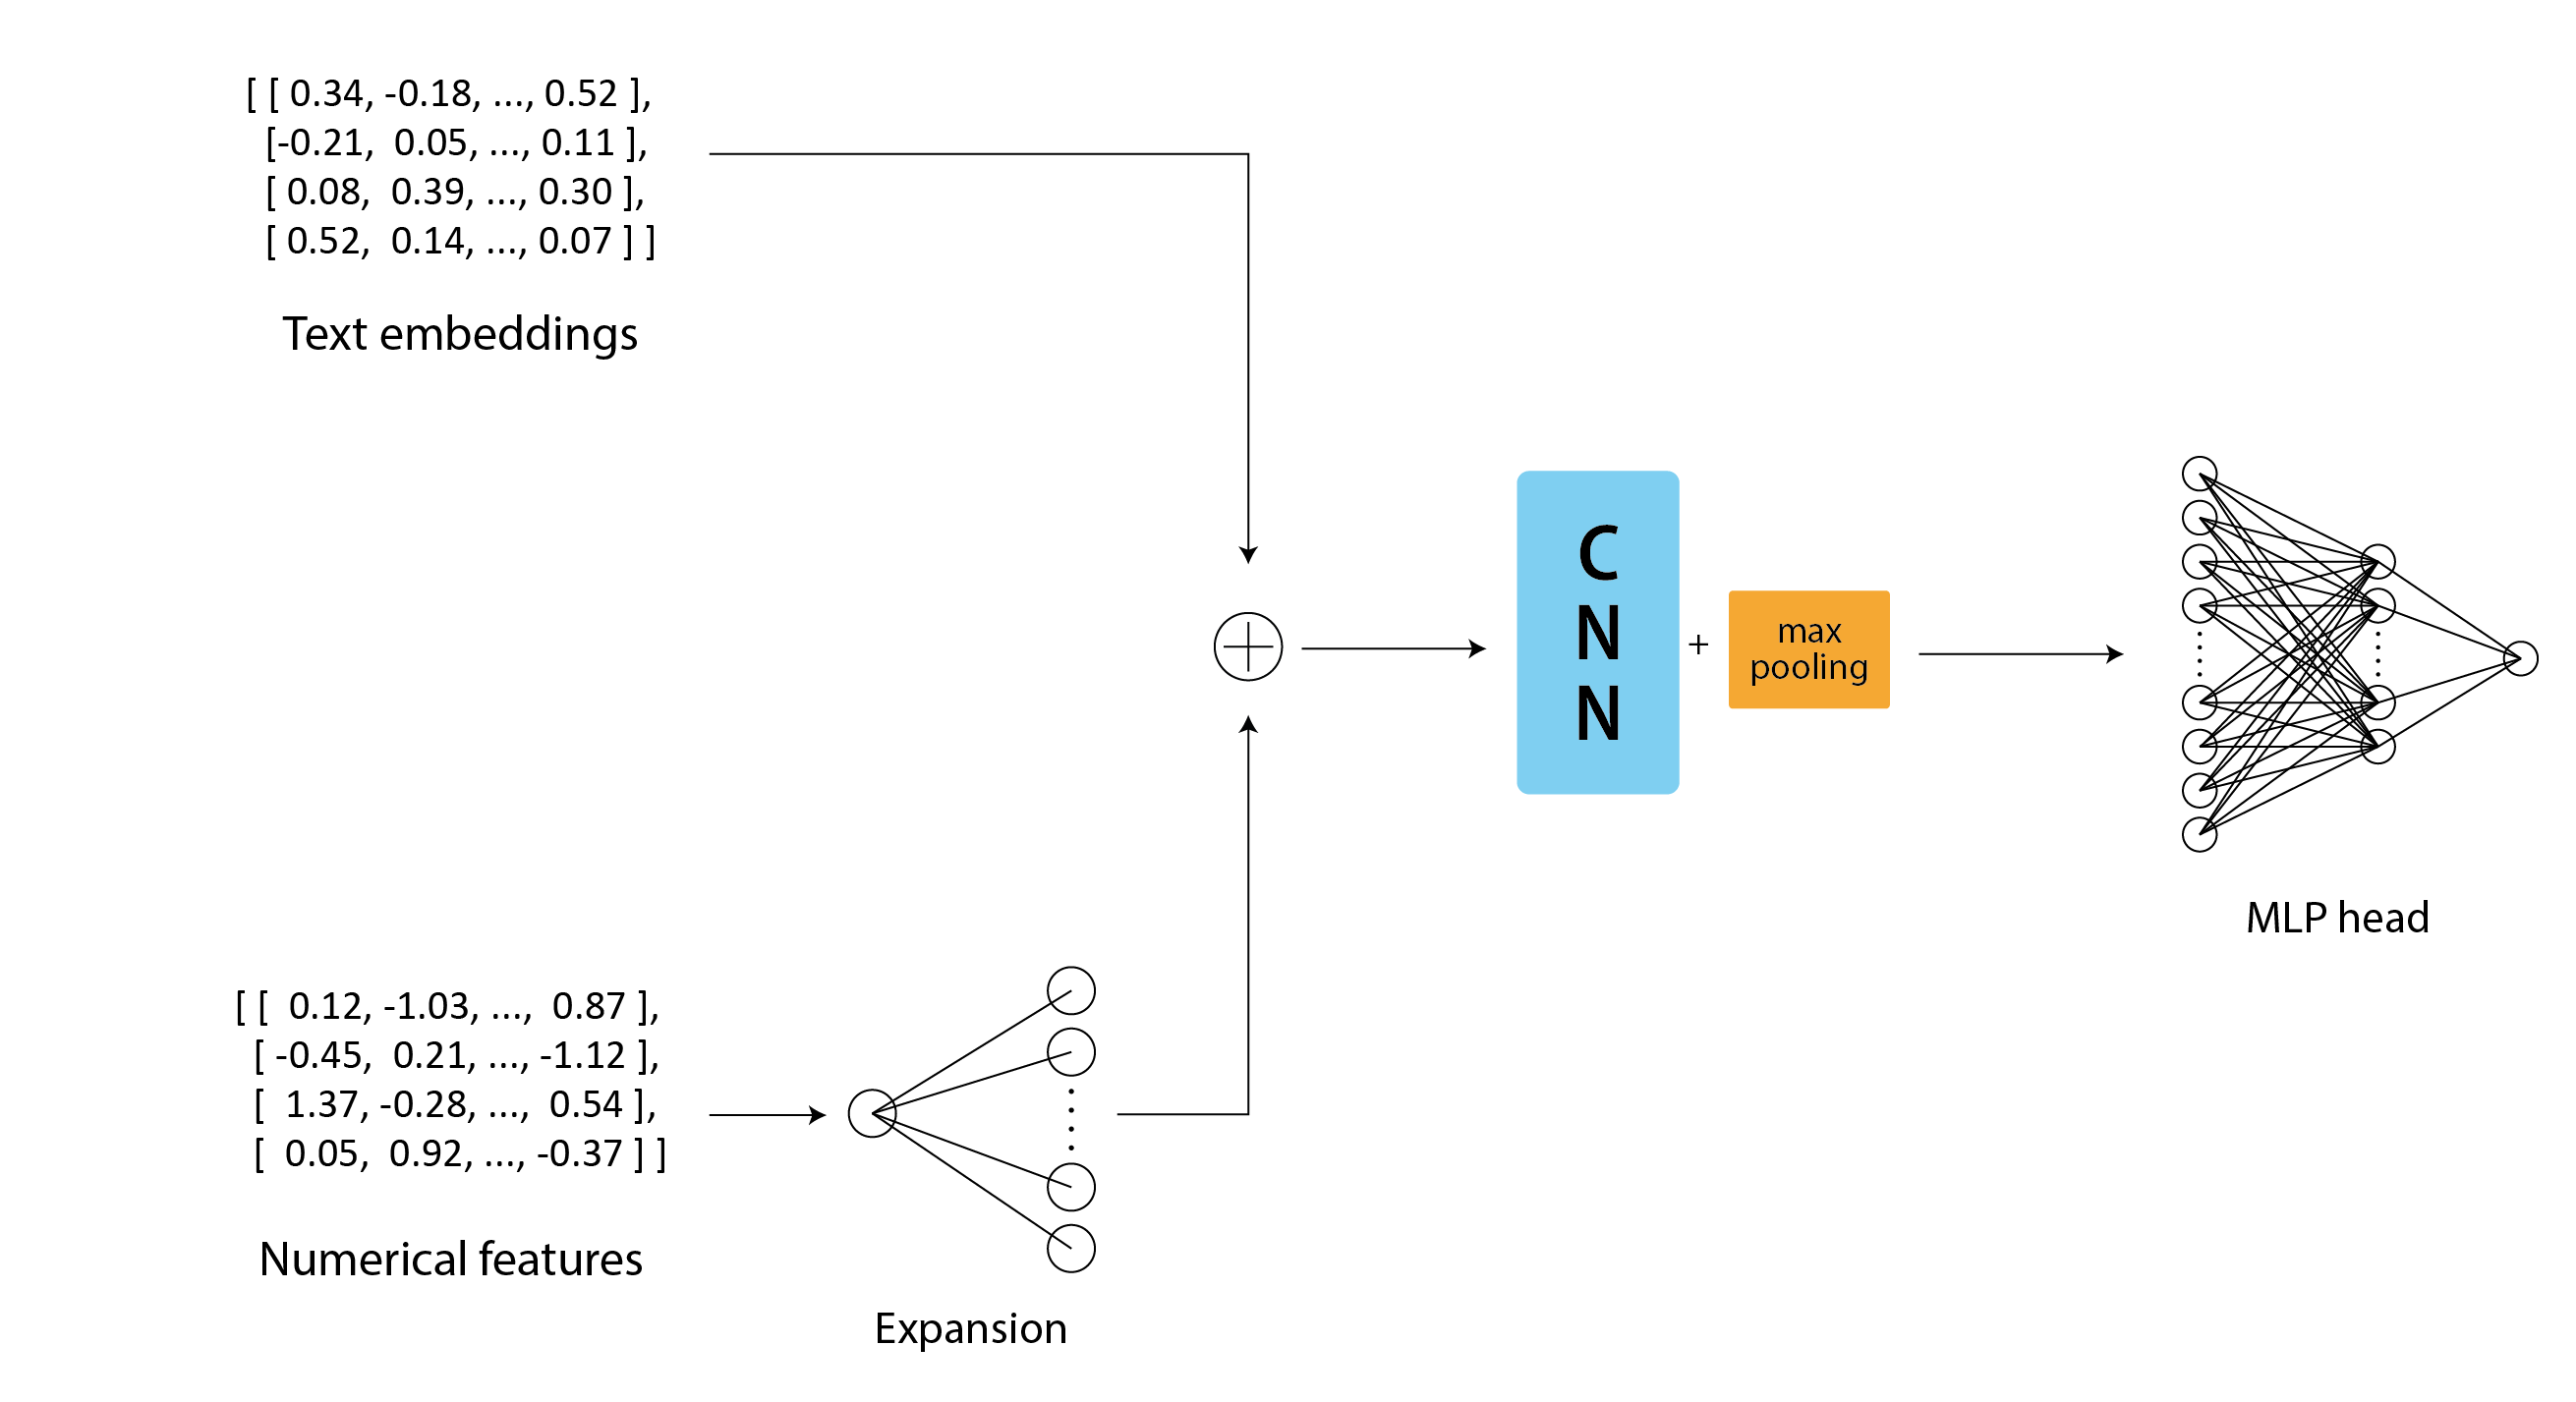
\includegraphics[width=1.1\textwidth]{./img/2_seq_model.png}
	\caption{CNN-based model} \label{CNN}
\end{figure}

\subsubsection*{Model 5: transformer encoder}
\addcontentsline{toc}{subsubsection}{Model 5: transformer encoder}

This model replaces convolutional layers with a bidirectional Transformer encoder. As in previous models, we first embed the five numeric features of each tweet $T_{ij}$ into a 32-dimensional space and then fuse them with the text representation, obtaining $\mathbf{x}_{ij}\in\mathbb{R}^{800}$. A linear projection then maps $\mathbf{x}_{ij}$ to the Transformer width $d_\text{model}=256$:
\[
\mathbf{z}_{ij} = W_p \mathbf{x}_{ij} + \mathbf{b}_p\in\mathbb{R}^{256}.
\]

To each element of sequence $(\mathbf{z}_{i1},\dots,\mathbf{z}_{i\ell})$ we add a learned positional embedding $\mathbf{p}_j\in\mathbb{R}^{256}$, following already established practice\footcite{devlin2019}. The position-aware series is then passed through a single layer Transformer encoder:
\[
\mathbf{Z}_i = \mathrm{Encoder}\!\left( (\mathbf{z}_{ij}+\mathbf{p}_j)_{j=1}^{\ell} \right),
\]
with $8$ heads and feed-forward dimension $512$. Padding positions are masked during self-attention. Since encoder's output shape is the same as input -- that is, $\mathbf{Z}_i \in \mathbb{R}^{\ell\times256}$ -- we aggregate over sequence lenght by max pooling to obtain $\mathbf{h}_i\in\mathbb{R}^{256}$. A two-layer perceptron produces the output score:
\[
\mathbf{u}_i=\phi\!\left(W_1\mathbf{h}_i+\mathbf{b}_1\right)\in\mathbb{R}^{64},\qquad
\hat{y}_i = \sigma({\mathbf{w}_2^\top \mathbf{u}_i + b_2}).
\]

As in the previous cases, the model is trained using a binary cross-entropy loss. Below is a visualization of model architecture.\\

\begin{figure}
	\centering
	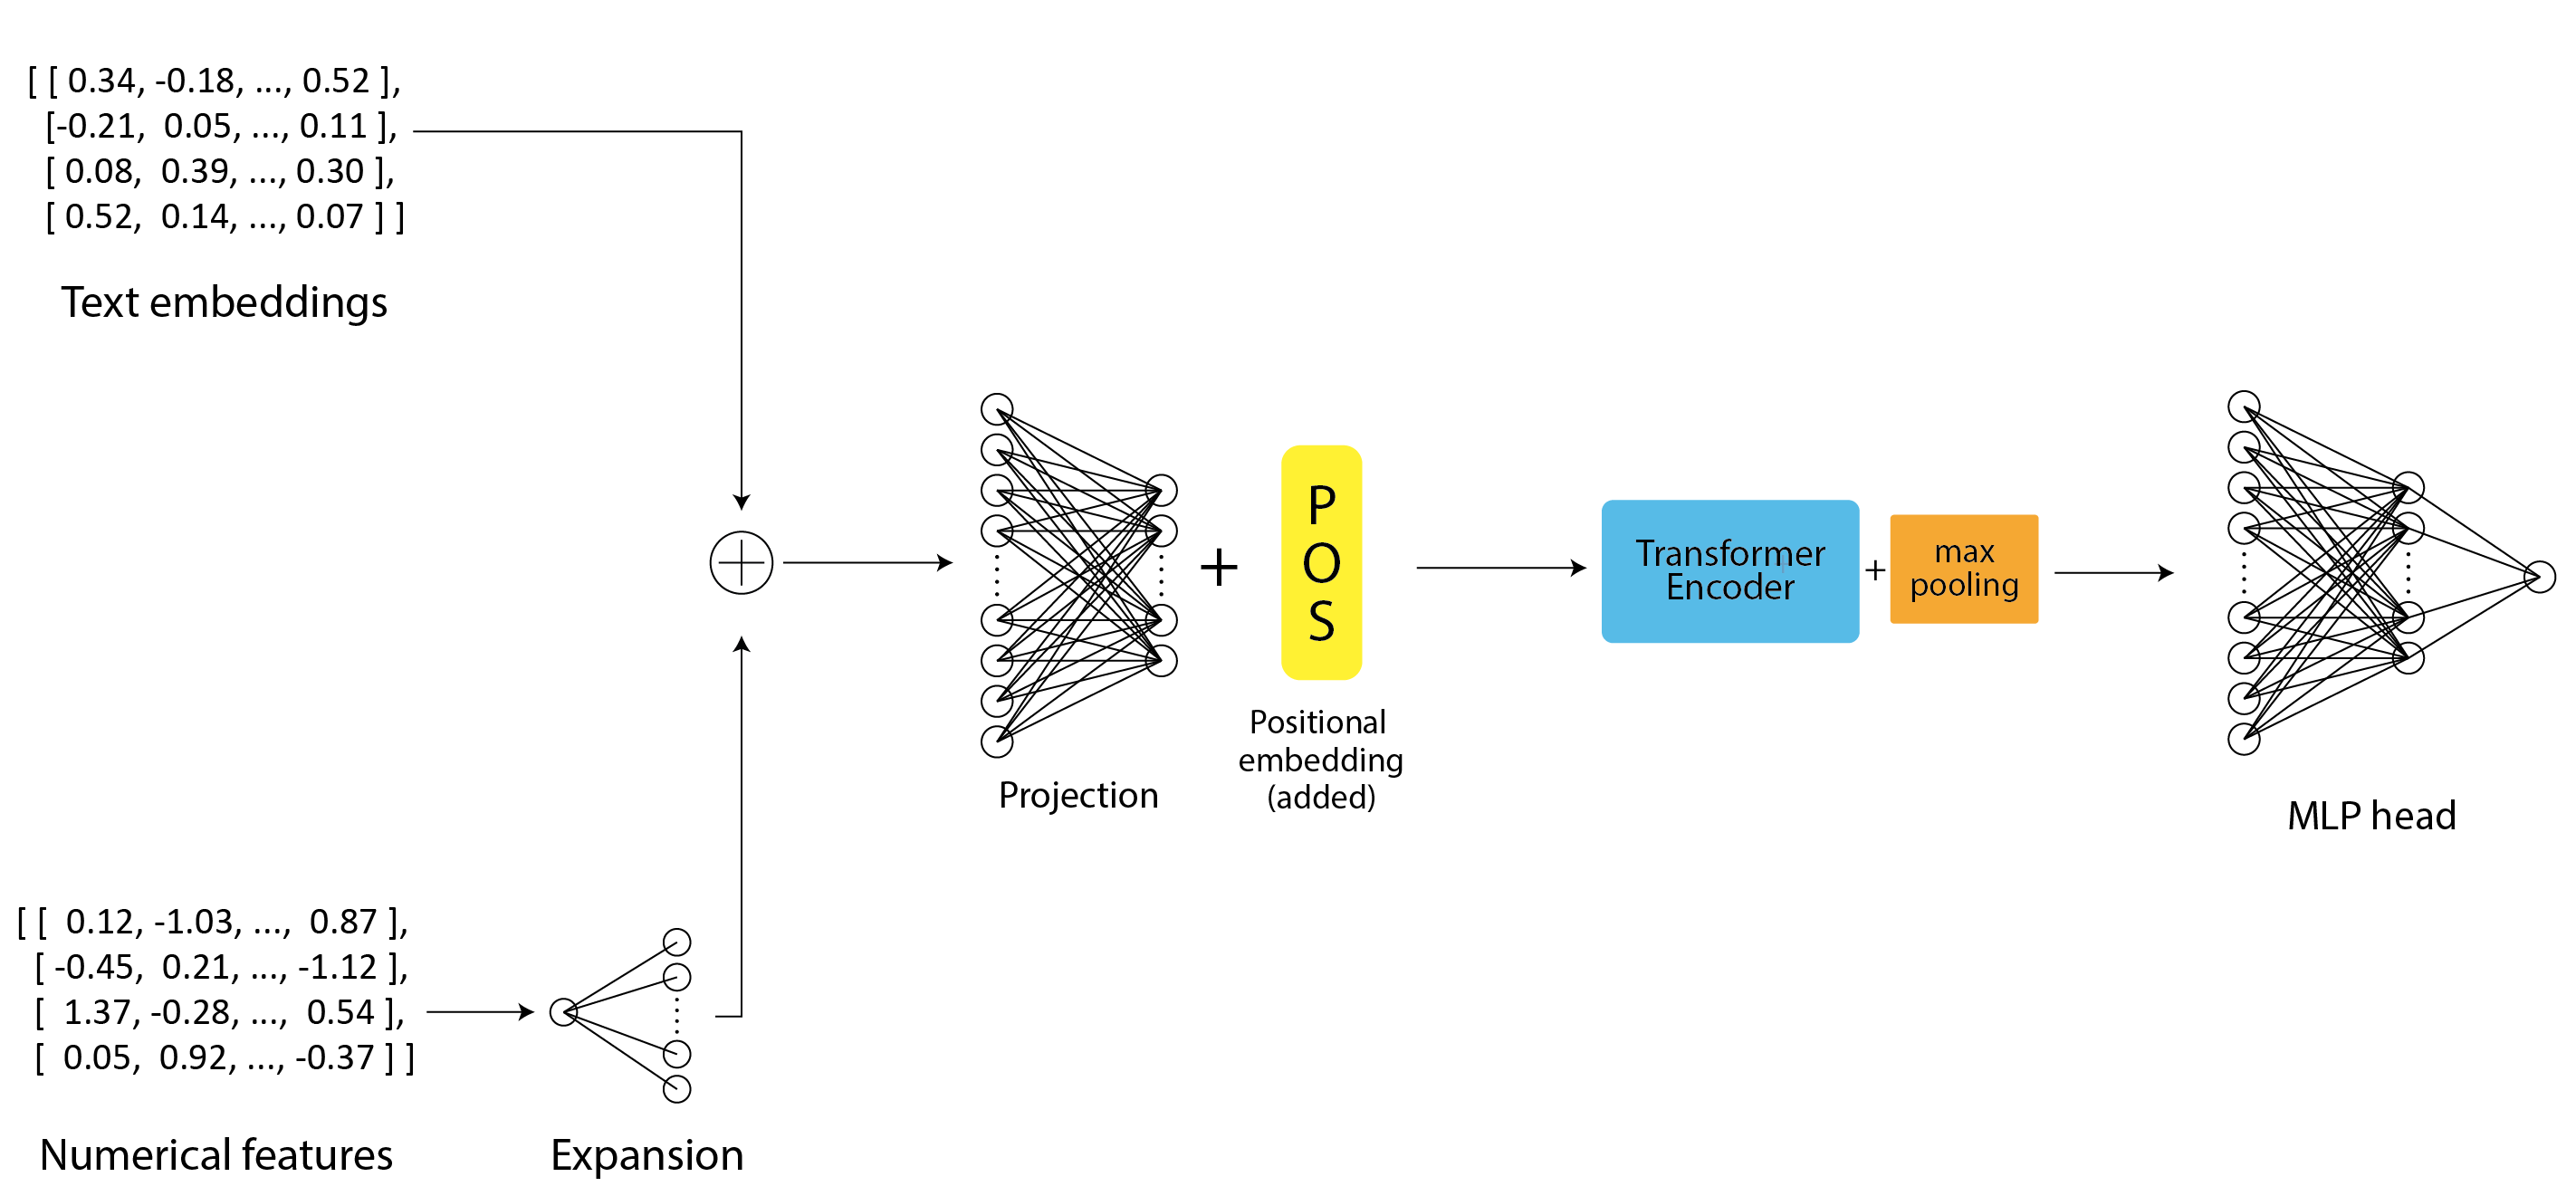
\includegraphics[width=1.1\textwidth]{./img/3_seq_model.png}
	\caption{Transformer encoder-based model}
\end{figure}


During these experiments, another aspect was also analyzed. We took the first model (bidirectional GRU), kept the same architecture, and modified the input data. In one case, we removed the numerical features from each tweet and left the embeddings generated with BERT, thus obtaining $T_{ij} = (\text{text}_{ij})$. In another, we did the exact opposite, removing the BERT embeddings and leaving the numerical features -- thus  $T_{ij} = (\Delta t_{ij},\ \text{followers}_{ij}, \allowbreak \text{following}_{ij},\ \text{verified}_{ij},\, \allowbreak \text{likes}_{ij} )$. In this way, we verified the contribution of the two types of data to the model identification activity. Results are presented in the next chapter.

\vspace{2em}

\subsection{Virality prediction}
\subsubsection*{Input data}
\addcontentsline{toc}{subsubsection}{Input data}

The dataset for this task is the same set of $N = 578$ tweet series
\[
\mathcal{T} = \{ S_1, S_2, \dots, S_N \}
\]
described in the previous subsection. Each tweet $T_{ij} \in S_i$ is represented as:
\[
T_{ij} = \left( \text{text}_{ij},\ \Delta t_{ij},\ \text{followers}_{ij},\ \text{following}_{ij},\ \text{verified}_{ij},\ \text{likes}_{ij} \right)
\]

As discussed in the previous chapter, virality is defined from the total number of likes $L_i$ collected by all tweets in $S_i$. Due to the small dataset size, we did not apply a high-percentile threshold as in the Evons dataset. Instead, a median-based split was used. Let $m_L$ be the median of the distribution $\{L_1, L_2, \dots, L_N\}$. The binary label $v_i$ assigned to each series $S_i$ is given by:
\[
v_i =
\begin{cases}
	1 & \text{if } L_i > m_L \quad \text{(viral)} \\
	0 & \text{otherwise} \quad \text{(non-viral)}
\end{cases}
\]
This ensures equal class representation, though it also means that ``viral'' corresponds to above-median performance rather than absolute high engagement.

The model's task is to predict the total number of likes $L_i$ for each series, so the $\text{likes}_{ij}$ feature was retained in the tweet representation as it doesn't introduce any data leakage. Text fields $\text{text}_{ij}$ were converted to 768-dimensional \texttt{RoBERTa} embeddings $\mathbf{d}_{ij}$, while non-binary numeric features ($\Delta t_{ij}$, $\text{followers}_{ij}$, $\text{following}_{ij}$, $\text{likes}_{ij}$) underwent the same log transformation and standardization procedure described on page~\pageref{model 3}. The binary feature $\text{verified}_{ij}$ was left unchanged. All sequences were then padded or truncated to a fixed length $\ell$.

\subsubsection*{Problem definition}
\addcontentsline{toc}{subsubsection}{Problem definition}

The problem is formulated as binary classification:
\[
f: (S) \mapsto v
\]
where $S_i$ is the tweet series and $v_i \in \{0,1\}$ indicates whether the series is classified as viral.

As with fake news detection, the sequential nature of the data means that temporal order, inter-tweet intervals, and user metrics can contribute to the prediction. In this case, however, the label construction guarantees class balance, that's why we did not need to try balancing strategies as undersampling or oversampling. In any case, we still used a weighted loss to take into account minor imbalances in the creation of the training and test datasets.\\ For this task, we used the same models described in \ref{fakenewsdata_detection_models}.

\chapter{Results}
In this chapter, the results of the methods described above will be presented and discussed. The structure of this section will follow that of the previous chapter. First, we will analyze the results relating to the Evons dataset, starting in particular with fake news detection and then moving on to virality prediction. Next, we will examine the results relating to the FakeNewsNet dataset, in the same order of task.\\

Before proceeding, it is worth addressing a general point. As already mentioned, this work did not involve extensive research into the hyperparameters of the various models tested. Manual tests were carried out to find satisfactory combinations. In the case of similar models, the same combinations were retained to allow for greater comparability of results. This does not guarantee that these are the best possible combinations. It is highly likely that there are different combinations of hyperparameters that can ensure better performance of the models examined. However, from the manual tests that were carried out, the use of different hyperparameters changes the results relatively little. We are talking about a few percentage points, which are unlikely to affect the general conclusions of this work. 

Finally, it is worth dwelling on the metrics used for evaluation. Let:

\begin{itemize}
	\item \textbf{True Positive (TP)}: number of positive instances correctly classified as positive.  
	\item \textbf{True Negative (TN)}: number of negative instances correctly classified as negative.  
	\item \textbf{False Positive (FP)}: number of negative instances incorrectly classified as positive.  
	\item \textbf{False Negative (FN)}: number of positive instances incorrectly classified as negative.  
\end{itemize}

Based on these quantities, the following evaluation metrics are used in this work:  

\begin{itemize}
	\item \textbf{Accuracy}:  
	$$
	\text{Accuracy} = \frac{TP + TN}{TP + TN + FP + FN}
	$$
	Measures the overall proportion of correctly classified instances among all instances.  
	
	\item \textbf{Balanced Accuracy}:  
	$$
	\text{Balanced Accuracy} = \frac{1}{2}\left(\frac{TP}{TP + FN} + \frac{TN}{TN + FP}\right)
	$$
	Computes the average recall across classes, mitigating the impact of class imbalance.  
	
	\item \textbf{Precision}:  
	$$
	\text{Precision} = \frac{TP}{TP + FP}
	$$
	Proportion of correctly predicted positive instances among all predicted positives.  
	
	\item \textbf{Recall (Sensitivity)}:  
	$$
	\text{Recall} = \frac{TP}{TP + FN}
	$$
	Proportion of correctly identified positives among all actual positives.  
	
	\item \textbf{F1-score}:  
	$$
	F1 = 2 \cdot \frac{\text{Precision} \cdot \text{Recall}}{\text{Precision} + \text{Recall}}
	$$
	Harmonic mean of precision and recall, providing a balanced measure between the two.  
	
	\item \textbf{ROC AUC}:  
	$$
	\text{ROC AUC} = \int_0^1 TPR(FPR) \, dFPR
	$$
	Area under the Receiver Operating Characteristic curve, which plots the True Positive Rate (TPR) against the False Positive Rate (FPR) at different thresholds.  
	A perfect model achieves $\text{ROC AUC} = 1$, while a random (uninformative) classifier typically yields $\text{ROC AUC} = 0.5$ in the binary case.  
\end{itemize}

In classification tasks, evaluation metrics can be computed in different ways. Common approaches include \textit{macro averaging} (computing the metric independently for each class and averaging), \textit{micro averaging} (aggregating contributions of all classes before computing the metric), or reporting the score for a single class of interest. This is particularly relevant in the case of imbalanced datasets.

In this work, we adopt the last approach and report results only for the positive class, as it represents the most relevant case in the considered tasks, following standard practice when dealing with binary classifications. All metrics are calculated on test sets, e.g. data points not seen by the model during training. 

\section{Evons}

Now let's move on to the presentation of the results relating to the Evons dataset. But first, a few notes concerning both tasks carried out on these data. All models were trained using a k-fold cross-validation technique. This is a widely used strategy that involves dividing the dataset into $k$ subgroups. The model is then trained on a different subgroup each time up to $k-1$ (the penultimate one), while the remaining one is used as a test, so that each fold serves once as the test set. At each training session, the model weights are reinitialized. This technique is used to reduce the bias associated with a single test train split (for example, a random case in which the test dataset contains data points that are particularly easy for the model to predict). In particular, a stratified k-fold strategy was used: subgroups are created in such a way as to respect the same distribution of classes -- for example, true or false; viral or non-viral -- as the entire dataset. In other words, if the original dataset has 5\% of posts labeled as viral and 95\% of posts labeled as non-viral, then each subgroup will have the same proportions. \\
Following research standards, we set $k=10$. For each fold, we selected the epoch scores with the best F1.\\

To get a better idea of the performance of the tested models, we also calculated the results of some simpler statistical models as baselines. Specifically, we tried:

\begin{itemize}
	\item Dummy stratified classifier: a model that calculates the frequency of classes in the training data and makes random predictions in the inference phase based on the calculated frequencies.
	
	\item Logistic regression: a linear model that applies a sigmoid function to a weighted sum of the input features, making it equivalent to a one-layer neural network.
	
	\item Random Forest Classifier: a model that creates several Decision Tree Classifiers and, during the inference phase, selects the class predicted by the majority of decision trees.
\end{itemize}

These baseline models take as input data the concatenated \texttt{RoBERTa} embeddings of articles' title and caption.

\subsection{Fake news detection}

\begin{table}[h!]
	\centering
	\caption{Model Performance Comparison  on fake news detection (Cross-Validation Averages) -- Evons}
	\label{tab:results_evons_detection}
	\vspace{0.5em}
	\begin{tabular}{lcccccc}
		\hline
		\textbf{Model} & \textbf{Accuracy} & \textbf{Balanced Acc.} & \textbf{F1} & \textbf{Precision} & \textbf{Recall} & \textbf{ROC AUC} \\
		\hline
		MLP & 0.991 & 0.991 & 0.990 & 0.990 & 0.990 & 0.999 \\
		\hline
		Dummy (Stratified)        & 0.501 & 0.498 & 0.457 & 0.458 & 0.456 & 0.501 \\
		Logistic Regression       & 0.972 & 0.971 & 0.969 & 0.971 & 0.967 & 0.996 \\
		Random Forest             & 0.932 & 0.931 & 0.926 & 0.925 & 0.927 & 0.983 \\
		\hline
	\end{tabular}
\end{table}

The results of the models are presented in table \ref{tab:results_evons_detection}. There are a few things to note. The first is that this is clearly an easy task for the different models. Even the baseline models perform very well. This is probably due to the ability of the embeddings created by \texttt{RoBERTa} to model the differences between the two classes. To verify this possibility, we performed a principal component analysis on BERT embeddings of article titles and descriptions to visualize their variance. 

\begin{figure}[h!]
	\centering
	\subfigure[Titles' embeddings]{
		{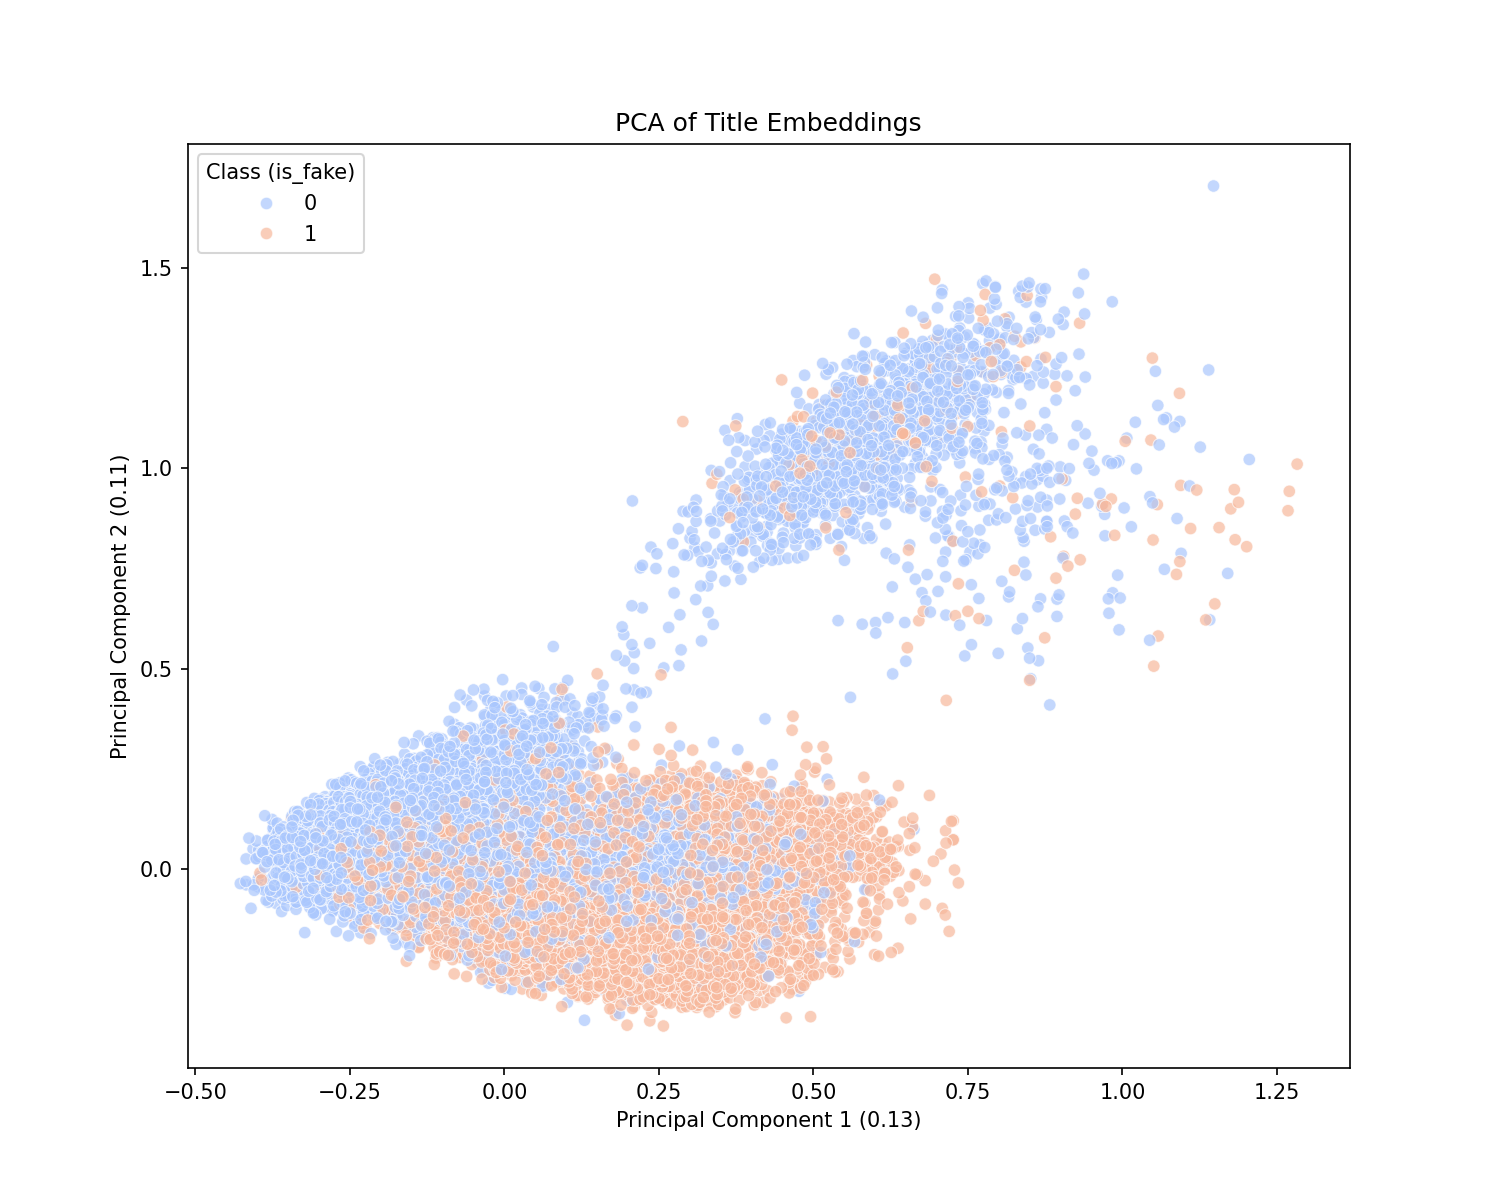
\includegraphics[scale=0.5]{./img/pca_title_embeddings.png}}
	} \\
	\subfigure[Captions' embeddings]{
		{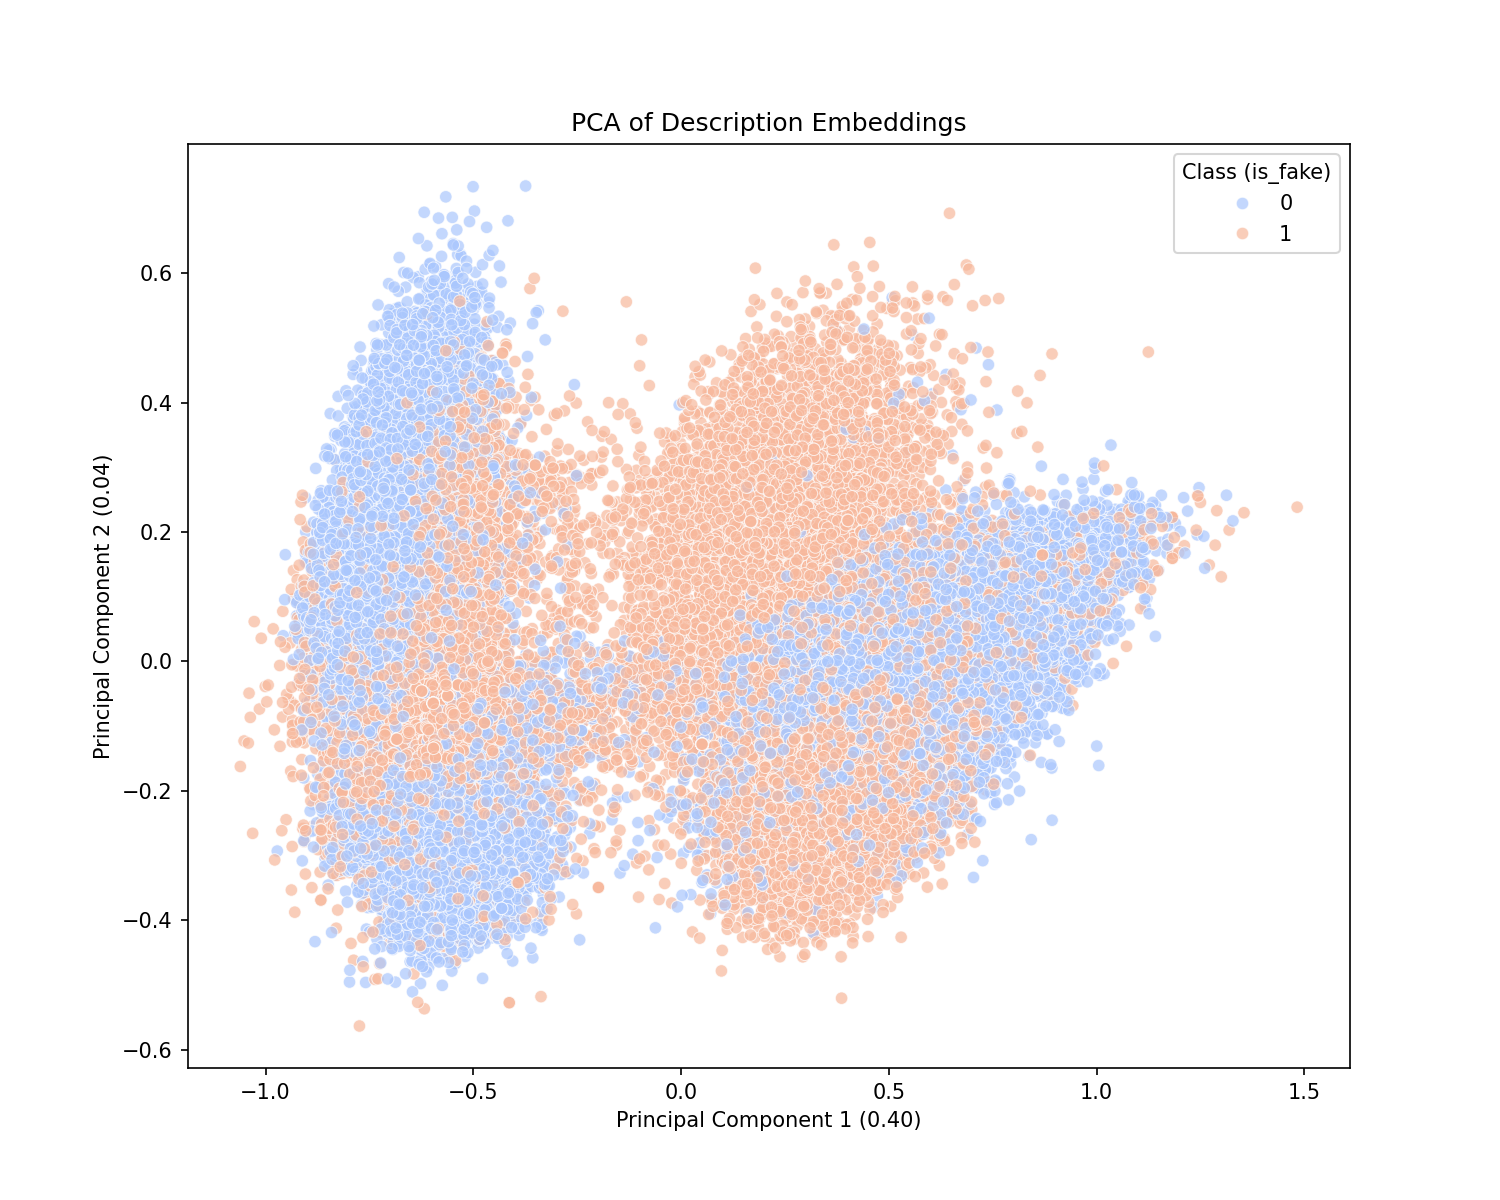
\includegraphics[scale=0.5]{./img/pca_description_embeddings.png}}
	}
	\vskip -0.5em
	\caption{PCA visualizations of titles and caption embeddings}
	\label{fig:pca_embs}
	\vspace{-0.1cm}
\end{figure}

As shown in Figure~\ref{fig:pca_embs}, the embeddings of article titles form different clusters -- even though with some important overlaps. This indicates that titles alone carry strong discriminative information between fake and real news, which explains the strong performance of even simple linear models such as logistic regression. In contrast, the embeddings of article captions exhibit more overlap between classes, except for a central group of fake articles, with less distinct separation in the principal component space. The PCA results partly confirm that RoBERTa embeddings encode class differences effectively, making fake news detection a relatively straightforward classification task.\\

Beyond its good overall performance, the MLP model presents the best results: f1, precision, and recall of 0.99. These are practically perfect scores. Compared to the baseline model with the best performance, logistic regression, MLP has two more points on average across all metrics. This small difference can be understood as the merit of non-linearity: this is the main difference between the two models. While logistic regression is a linear method (the only non-linear operation is the sigmoid function, which is only applied to the output), MLP introduces non-linearity with activation functions -- GELU in our case -- in the hidden layers. Random Forest, even though it is a non-linear model as well, has worse performances than MLP. That is due to the way the model works -- in particular, how decision trees work -- and it shows that not \textit{all kind} of non-linearity can guarantee good performances.

\FloatBarrier

\subsection{Virality prediction}

\begin{table}[H]
	\centering
	\caption{Model Performance Comparison on virality prediction (Cross-Validation Averages) -- Evons}
	\vspace{0.5em}
	\label{tab:results_evons_virality}
	\begin{tabular}{lcccccc}
		\hline
		\textbf{Model} & \textbf{Accuracy} & \textbf{Balanced Acc.} & \textbf{F1} & \textbf{Precision} & \textbf{Recall} & \textbf{ROC AUC} \\
		\hline
		MLP        & 0.885 & 0.712 & 0.312 & 0.224 & 0.519 & 0.842 \\
		Source emb.     & 0.865 & 0.756 & 0.322 & 0.217 & 0.635 & 0.869 \\
		Avg. engagement     & 0.869 & 0.751 & 0.322 & 0.218 & 0.621 & 0.867 \\
		Gating model  & 0.869 & 0.751 & \textbf{0.323} & 0.219 & 0.620 & 0.868 \\
		\hline
		Dummy (Stratified)        & 0.905 & 0.500 & 0.049 & 0.049 & 0.049 & 0.501 \\
		Logistic Regression       & 0.761 & 0.783 & 0.252 & 0.150 & 0.807 & 0.866 \\
		Random Forest             & 0.855 & 0.699 & 0.266 & 0.178 & 0.526 & 0.811 \\
		\hline
	\end{tabular}
\end{table}

In the case of virality prediction, the overall picture is quite different. The scores are generally much lower. No model achieves an F1-score greater than 0.32. This is due to several factors. First, the task itself is tricky: whether a post goes viral often depends on external factors that aren’t captured by the text alone -- for example, breaking news, trending debates, or political events. Second, the dataset is heavily unbalanced. Only 5\% of posts are labeled as viral, which makes it hard for models to learn meaningful patterns from so few examples.\\

Looking at these results, another general observation can be made. All models -- except for DummyClassifier -- achieve higher recall scores than precision scores. This means that the models are able to find a large proportion of posts that are actually viral. At the same time, however, they tend to consider viral many posts that actually are not. Furthermore, the model with the highest recall score is also the one with the lowest precision. This confirms the existence of a classic trade-off between the two scores.\\

All models score around an F1 score of 0.31-0.32, with the Gating model achieving the best score of 0.323. However, this is a negligible difference compared to other models' averages. The only notable gap is between neural network models and baselines: a difference of five or six points in the F1 score. Furthermore, introducing information about the source of the articles into the input data seems to make only a very limited contribution to the predictions: models that use source embeddings or the average number of likes per source achieve F1 scores that are only one point higher.\\

Finally, one aspect relating to the actual application of these models needs to be explored in greater depth. For simplicity, the main metric for evaluation and models comparison in this case was the F1 score. That is the reason why, for each fold, we selected the epoch scores with the best F1. Due to the way it is constructed, the F1 score is based on a balance between precision and recall. For example, the Gating model, which has the highest F1 score, has a precision of 0.219 and a recall of 0.620. Now let's imagine applying this model to a dataset of 100,000 posts, of which only 5,000 are actually viral. In this case, our model would predict that approximately 14,155 publications would go viral. Of these, only 3,100 would actually go viral. At the same time, there would be 1,900 publications that actually went viral but that our model would have considered non-viral -- almost 40\% of total truly viral posts.\\

In a real-world application of this model for identifying viral information and disinformation publications, considering so many truly viral posts as non-viral would be quite a problem. A model with higher recall but lower precision might actually be more useful, since it would catch more of the truly viral ones, even if it falsely labels many others as viral. Take the Logistic Regression model and apply it on the same dataset of 100,000 publications, knowing that it has a recall of 0.807 and a precision of 0.150. The model would predict that approximately 26,900 posts would go viral. Of these, only 4,035 would actually do so. At the same time, however, only 965 posts that actually went viral would be classified as non-viral -- around 20\% of total truly viral posts instead of 40\%. So, if we applied a model of this type in a real context, we could filter the dataset down to about a quarter of its size, knowing we’re still capturing most of the truly viral posts for further analysis.\\

Consequently, instead of F1, another criterion for comparing and selecting metrics for each fold would be more appropriate. One possible approach is to use $F\text{-}\beta$ a variant of F1 that allows weights to be assigned to precision and recall. Mathematically:

$$
F- = \frac{(w_{\text{Recall}} + w_{\text{Precision}}) \cdot \text{Precision} \cdot \text{Recall}}{w_{\text{Recall}} \cdot \text{Precision} + w_{\text{Precision}} \cdot \text{Recall}}
$$

where $w_{\text{Recall}}$ is the weight assigned to recall and $w_{\text{Precision}}$ is the weight assigned to precision.


When using the $F\text{-}\beta$ score, we can explicitly control how much importance we want to assign to recall versus precision. By adjusting the weights, we give more emphasis either to correctly identifying as many viral posts as possible (recall) or to avoiding false alarms when predicting virality (precision).\\

To explore how this trade-off affects the performance of our models, we experimented with different weight settings. In practice, this means that during training, for each fold of the cross-validation process, we monitored the $F\text{-}\beta$ score across epochs. At the end of each fold, we identified the epoch that achieved the highest $F\text{-}\beta$ score given the chosen weighting scheme. We then collected the metrics from these best-performing epochs. Finally, to make the results comparable across models, we averaged these metrics over all folds, just as we did in the previous evaluations. 

This procedure allowed us to systematically analyze how changing the balance between precision and recall influences the models’ overall effectiveness. The results of these experiments are shown in figure \ref{fig:ratios} , where we have expressed the average precision and recall of the various models as a function of the ratio between the weight of recall and the weight of precision (essentially, how much more important recall is than precision). 

\begin{table}[h!]
	\centering
	\caption{Performance of different models under an $F\text{-}\beta$ weighting scheme where recall is heavily prioritized (20 times more weight than precision). Cross-Validation averages. Baseline models are included for reference; their values remain unchanged as they were not trained with epoch selection based on $F\text{-}\beta$.}
	\label{tab:results_f_beta}
	\vspace{1em}
	\resizebox{\textwidth}{!}{
		\begin{tabular}{lccccccc}
			\hline
			\textbf{Model} & \textbf{Accuracy} & \textbf{Balanced Acc.} & \textbf{F1} & \textbf{Precision} & \textbf{Recall} & \textbf{ROC AUC} & \textbf{F$_\beta$} \\
			\hline
			MLP                & 0.688 & 0.772 & 0.219 & 0.126 & 0.865 & 0.853 & 0.673 \\
			Source emb.        & 0.740 & 0.787 & 0.245 & 0.144 & 0.839 & 0.868 & \textbf{0.681} \\
			Avg. engagement    & 0.728 & 0.784 & 0.239 & 0.139 & 0.847 & 0.867 & \textbf{0.681} \\
			Gating model       & 0.755 & 0.789 & 0.253 & 0.149 & 0.828 & 0.870 & 0.680 \\
			\hline
			Dummy (Stratified)  & 0.905 & 0.500 & 0.049 & 0.049 & 0.049 & 0.501 & 0.049 \\
			Logistic Regression & 0.761 & 0.783 & 0.252 & 0.150 & 0.807 & 0.866 & 0.668 \\
			Random Forest       & 0.855 & 0.699 & 0.266 & 0.178 & 0.526 & 0.811 & 0.481 \\
			\hline
		\end{tabular}
	}
\end{table}

Table \ref{tab:results_f_beta} reports the performance of the models under a weighting scheme where recall is given 20 times more importance than precision. As expected, this shift strongly favors recall: the models are now able to identify a much larger share of viral posts. However, this improvement comes at a clear cost -- precision drops significantly, meaning the models also generate many more false positives. For the sake of comparison, the table also includes the baseline models. Their metrics remain unchanged from the previous results, since these baselines were not trained with a procedure that allows selecting the best epoch per fold based on the $F\text{-}\beta$ score. 

Looking more closely at the results, we see that all models follow the same pattern compared to baselines: higher recall but lower precision. This confirms that the recall-precision trade-off cannot be solved universally. Instead, the most suitable balance depends on the practical requirements of the application. 

\begin{figure}[h!]
	\centering
	\subfigure[Precision values obtained when varying the weight ratio in the $F\text{-}\beta$ score]{
		{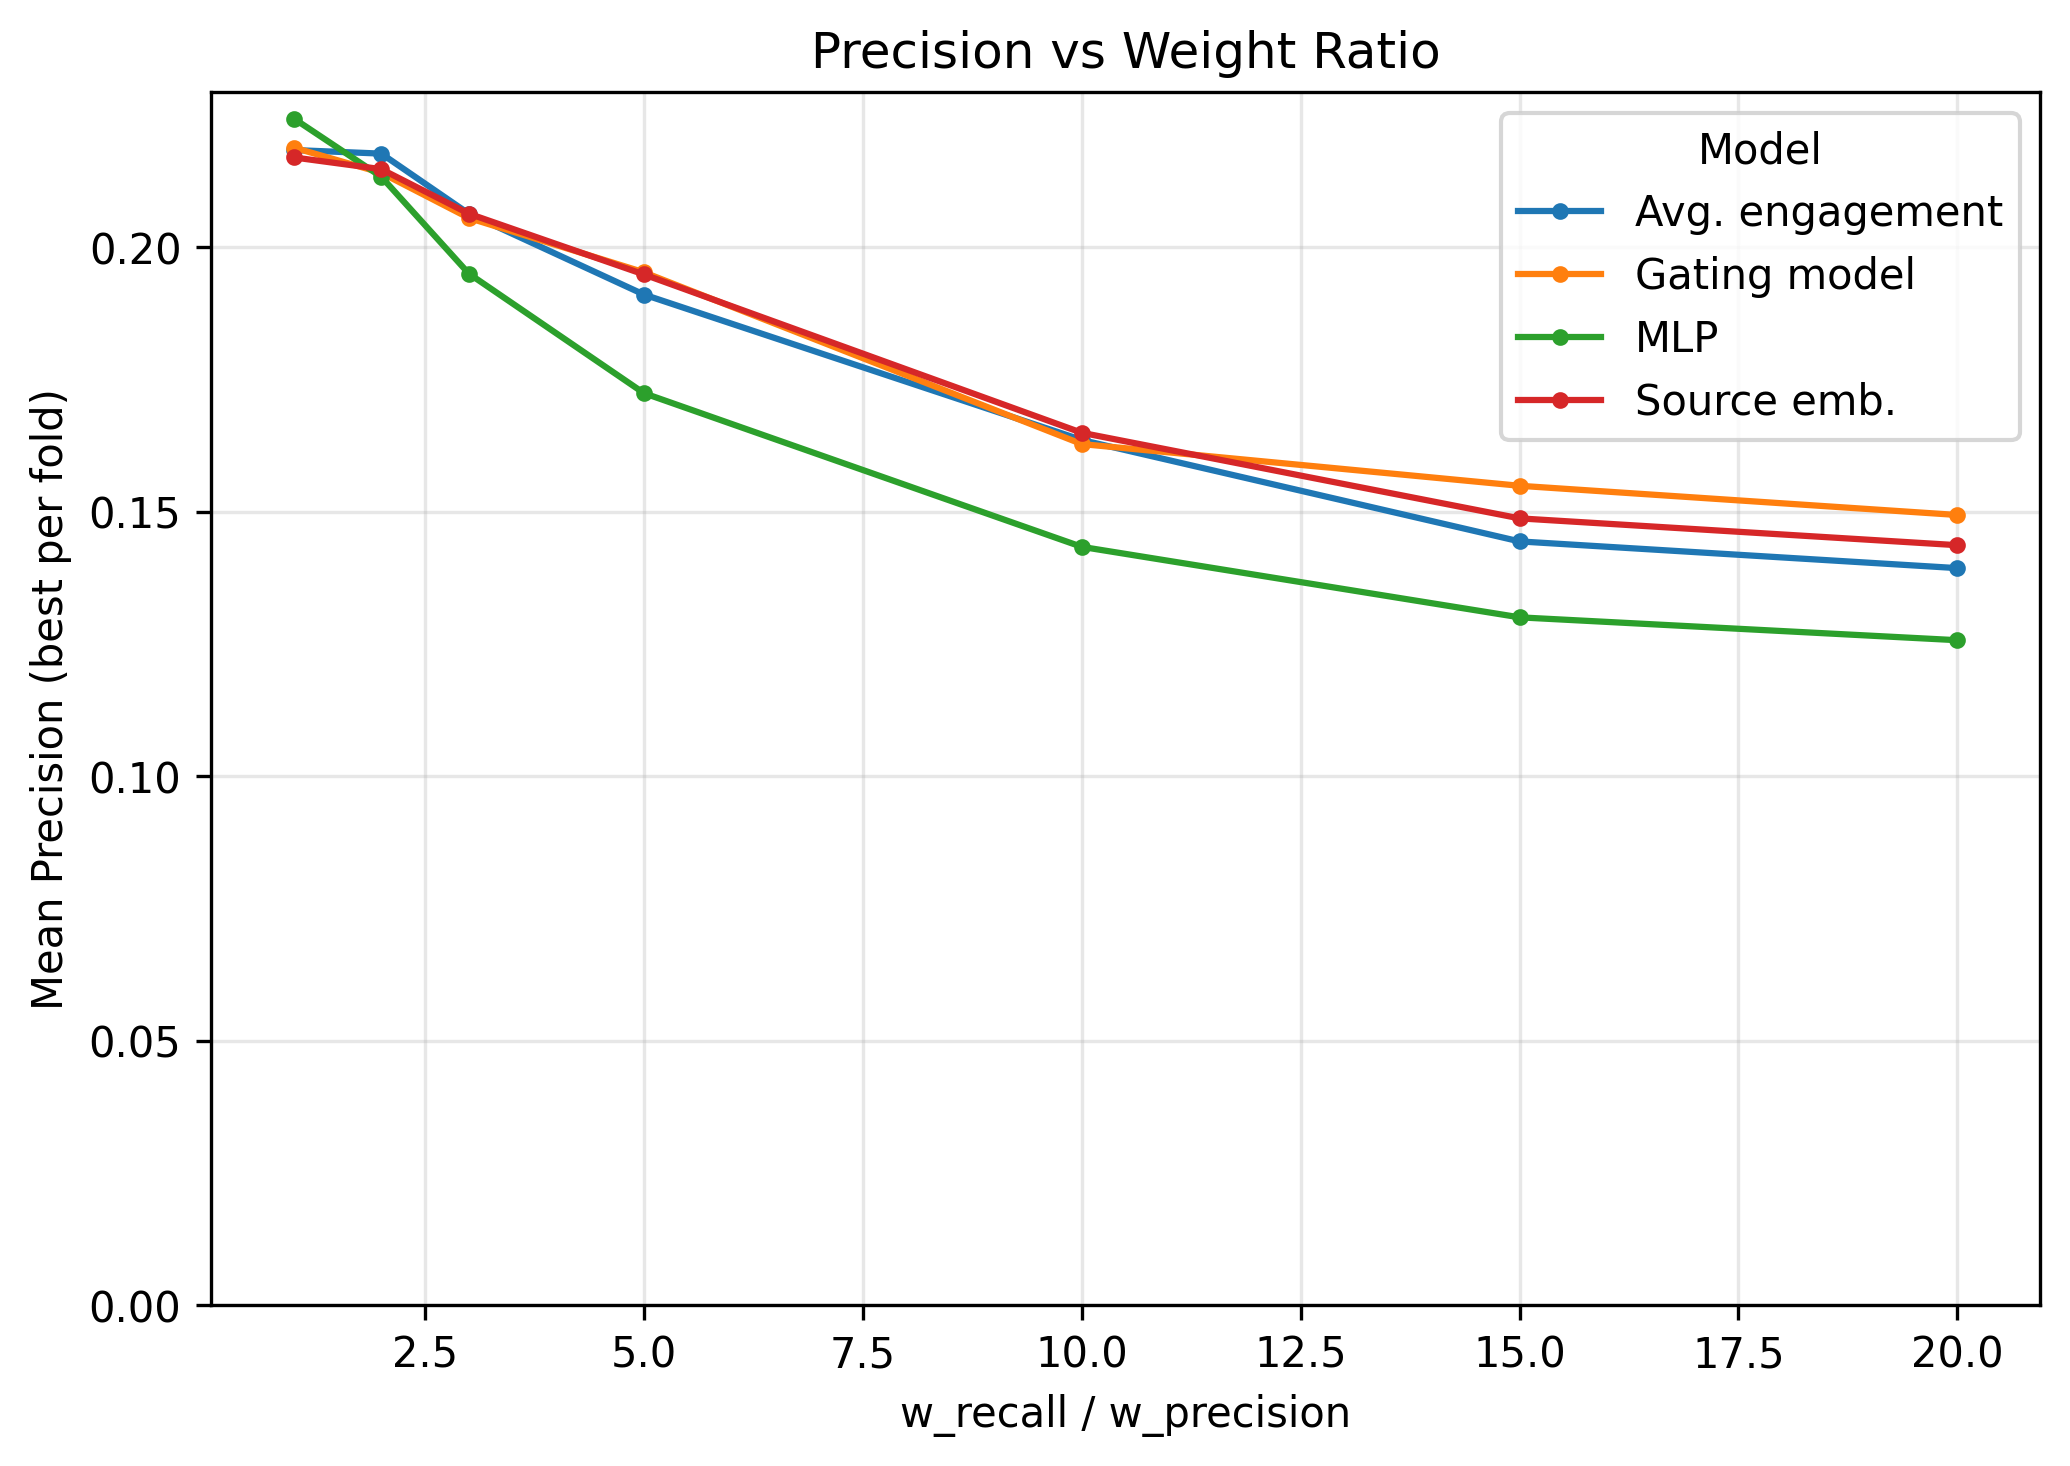
\includegraphics[scale=0.8]{./img/precision_vs_ratio.png}}
	} \\
	\subfigure[Recall values obtained when varying the weight ratio in the $F\text{-}\beta$ score]{
		{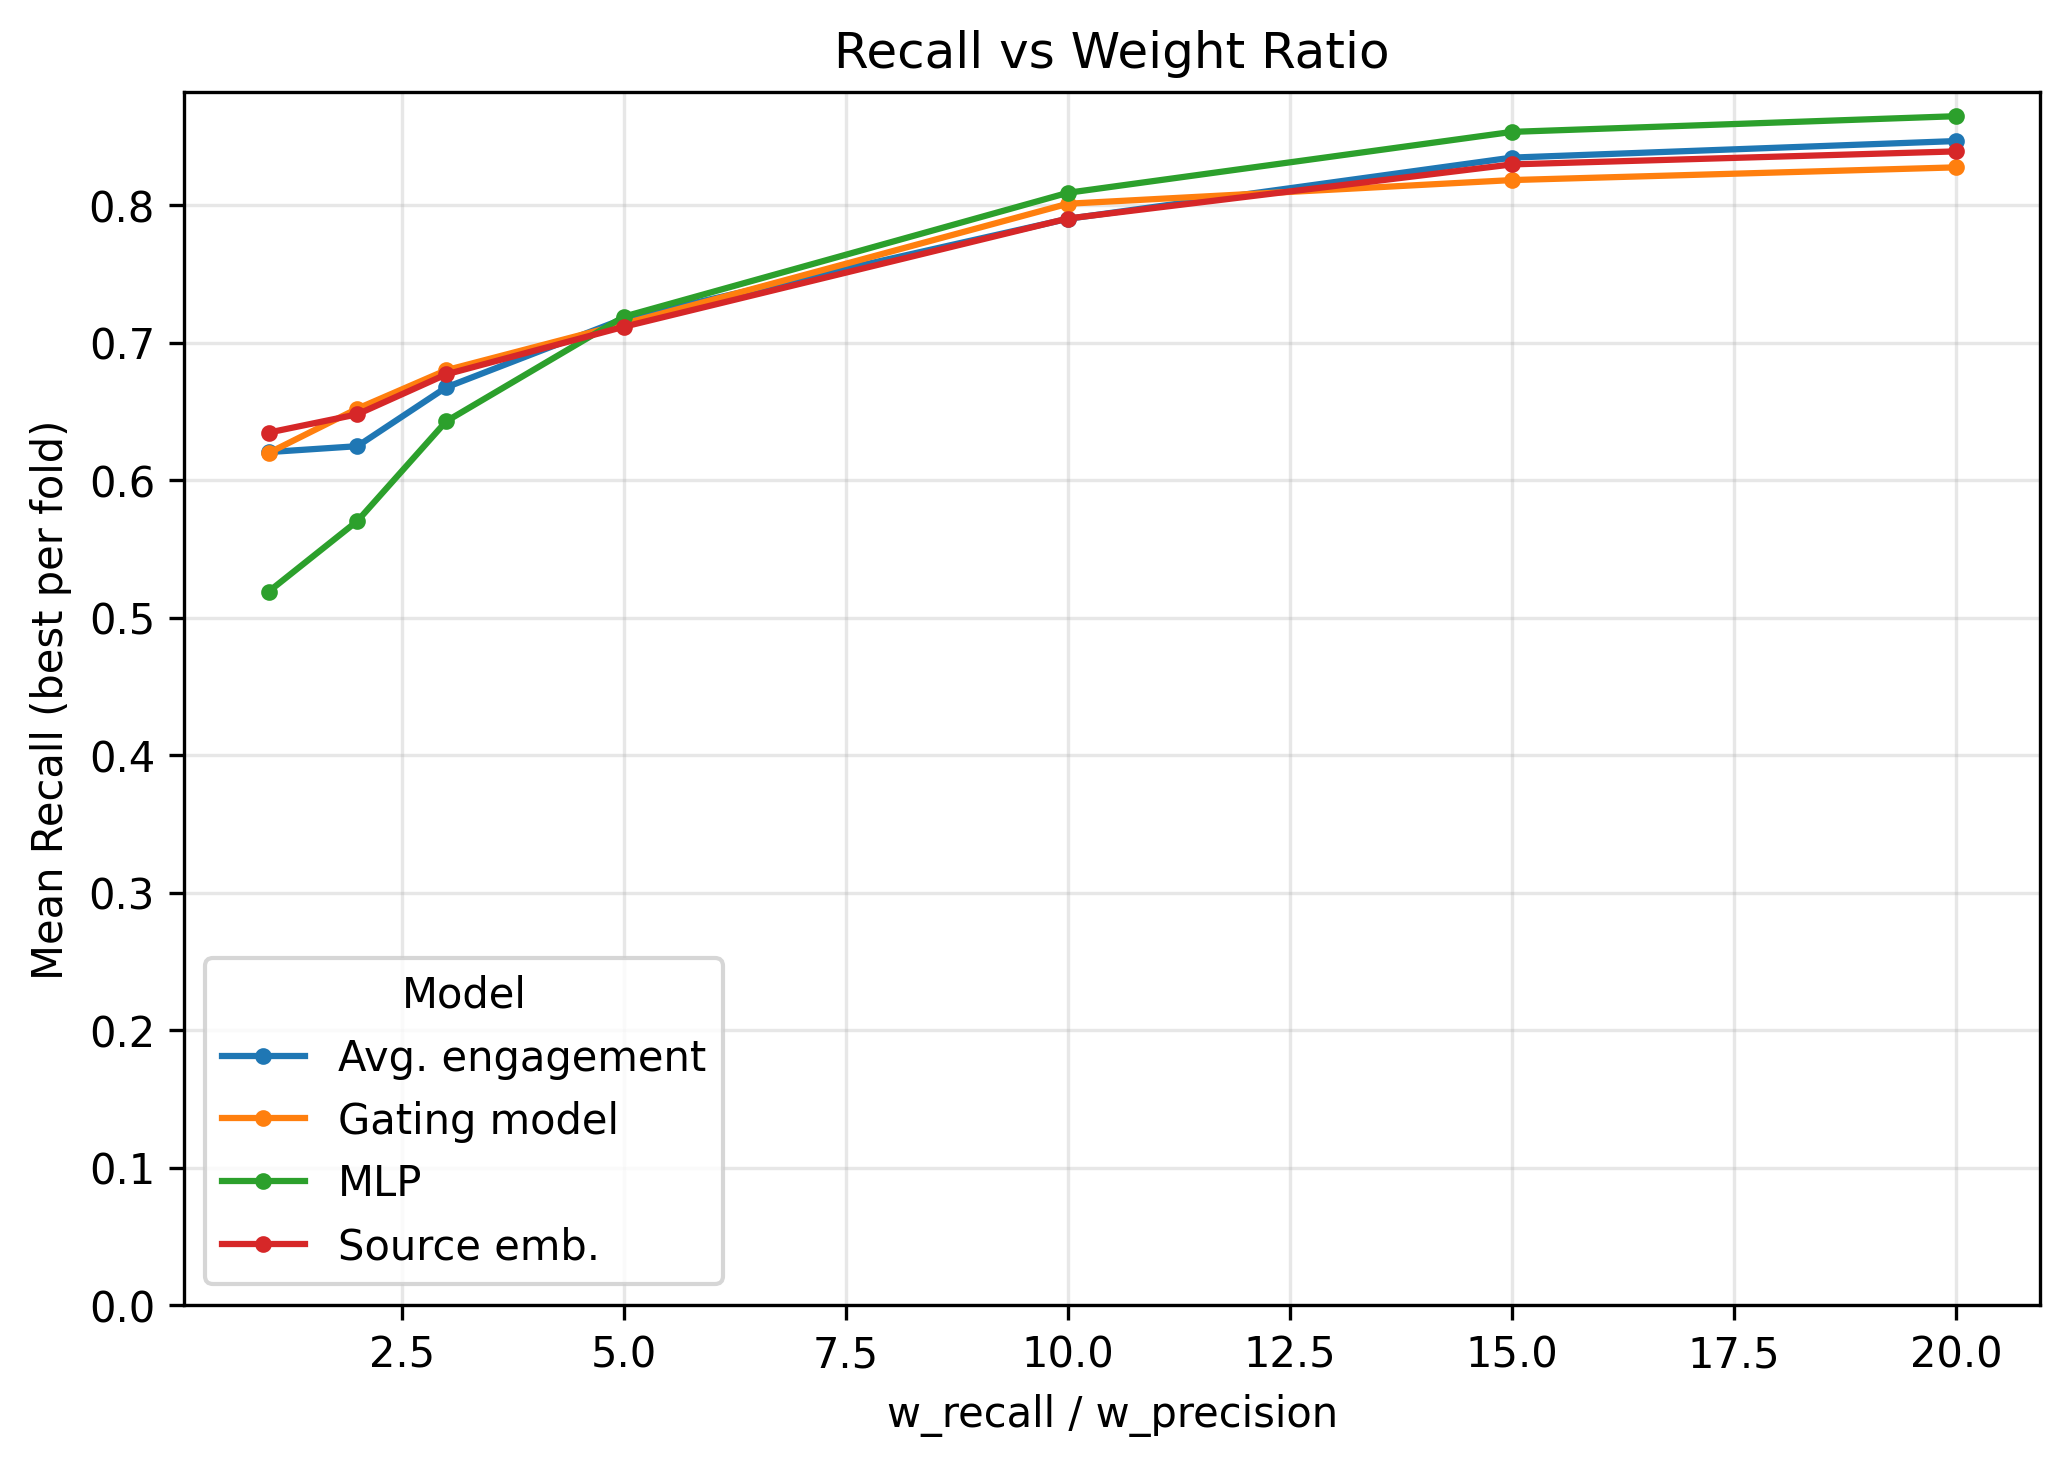
\includegraphics[scale=0.8]{./img/recall_vs_ratio.png}}
	}
	\vskip -0.5em
	\caption{Evolution of models’ precision and recall as a function of the weighting scheme in the $F\text{-}\beta$ score. By adjusting the balance between precision and recall during model selection, we can observe how the models shift their behavior: higher weights on recall lead to identifying more true viral posts (higher recall) but at the cost of precision, while lower weights have the opposite effect.}
	\label{fig:ratios}
	\vspace{-0.1cm}
\end{figure}

\section{FakeNewsNet}

We now present the results of our experiments on the FakeNewsNet: dataset for two tasks: fake news detection and virality prediction. Before showing the results, however, it is important to explain the validation strategy we used. Ordinarily, we would have used a k-fold cross-validation, as we did earlier. As we've already explained, in this method the dataset is divided into $k$ equally sized groups (called folds). The model is then trained on $k - 1$ folds and tested on the remaining fold, and this process is repeated $k$ times. Each fold serves once as the test set. For example, with $k = 10$, the dataset would be split into ten parts, each representing $10\%$ of the total. This approach works well for large datasets. For instance, in the case of the Evons dataset, which contains about 100,000 articles, each fold would still have around 10,000 examples -- large enough to ensure both training and testing are meaningful.  \\

However, the situation is very different for FakeNewsNet, which contains fewer than 600 articles in total. If we had applied 10-fold cross-validation here, each fold would contain fewer than 60 examples, making the training sets very small and the evaluation unreliable.  \\
To address this issue, we used an alternative method known as \emph{shuffle split cross-validation}. Instead of dividing the dataset into fixed folds, this method repeatedly splits the dataset into a training set and a test set at random. The process is repeated $n$ times, and in each iteration the model is trained and evaluated on a different random split. Importantly, across these repetitions, the entire dataset is used multiple times, sometimes for training and sometimes for testing, but always in different combinations. This provides a more stable and reliable evaluation when working with a small dataset like FakeNewsNet. We chose $ n=10$. \\

Another note concerns the length of the tweet series. So far, in the methods and data section, we have limited ourselves to indicating the length of the sequences artificially set as $\ell$. Now we can define it as $\ell=5$. The criteria for this decision will be explained after the presentation of the results.

The models used as baselines are the same as those used in the Evons dataset. For clarity, we list them here as well:

\begin{itemize}
	\item Dummy stratified classifier: a model that calculates the frequency of classes in the training data and makes random predictions in the inference phase based on the calculated frequencies.
	
	\item Logistic regression: a linear model that applies a sigmoid function to a weighted sum of the input features, making it equivalent to a one-layer neural network.
	
	\item Random Forest Classifier: a model that creates several Decision Tree Classifiers and, during the inference phase, selects the class predicted by the majority of decision trees.
\end{itemize}

These baseline models do not accept sequential data -- series of tweets, in our case. As a result, we processed the data before feeding it to them. For each tweet series, we calculated the mean, maximum, minimum, and standard deviation for each of the tweet 772 dimensions (768 dimensions representing the \texttt{RoBERTa} embeddings and the other five the numerical features, as described in the previous chapter), which results in a 3,088-features vector. Together, these statistics provide a condensed yet informative description of the entire sequence. However, relying only on summary statistics would ignore information about the temporal endpoints of the series, which can be particularly informative. To preserve this, we appended the complete feature vector of the first tweet and that of the last tweet in the sequence. This equals to 1544 additional features. At the end, for each series, we obtained a single flat representation, a vector of dimension 4636, that served as input data for baseline models.

\subsection{Fake news detection}

\begin{table}[h!]
	\centering
	\caption{Model Performance Comparison on fake news detection (Cross-Validation Averages) -- FakeNewsNet}
	\label{tab:results_fakenewsnet_detection}
	\vspace{0.5em}
	\begin{tabular}{lcccccc}
		\hline
		\textbf{Model} & \textbf{Accuracy} & \textbf{Balanced Acc.} & \textbf{F1} & \textbf{Precision} & \textbf{Recall} & \textbf{ROC AUC} \\
		\hline
		GRU          & 0.935 & 0.918 & 0.891 & 0.912 & 0.874 & 0.961 \\
		RNN                        & 0.941 & 0.926 & 0.901 & 0.919 & 0.886 & 0.963 \\
		LSTM                       & 0.936 & 0.916 & 0.891 & 0.921 & 0.866 & 0.963 \\
		CNN                       & 0.928 & 0.904 & 0.876 & 0.912 & 0.846 & 0.962 \\
		Transformer Encoder               & 0.945 & 0.927 & \textbf{0.906} & 0.933 & 0.883 & 0.965 \\
		\hline
		Dummy (Stratified)         & 0.578 & 0.499 & 0.300 & 0.300 & 0.300 & 0.499 \\
		Logistic Regression        & 0.939 & 0.929 & 0.899 & 0.896 & 0.906 & 0.971 \\
		Random Forest              & 0.920 & 0.893 & 0.861 & 0.902 & 0.826 & 0.956 \\
		\hline
	\end{tabular}
\end{table}


All models perform very well. This is not obvious when considering the imbalance between the two classes in the dataset. Only 30\% of the data points belong to the fake class (174 out of 578). As we observed earlier in the case of Evons, an imbalance in the dataset can easily lead to a deterioration in the performance of many types of models. Even logistic regression, which is a non-linear model, achieves an f1 score of 0.899. This suggests several things. First, that \texttt{RoBERTa} embeddings, together with numerical features, are very representative in themselves. In other words, there is no great need to resort to non-linear techniques to find hidden or particularly complex patterns in the data, because they are already very informative — obviously, this does not detract from the fact that textual embeddings are so rich because they were created with a deep, non-linear model. The second thing is that the method used to extract feature vectors from sequential data works well and does not result in a significant loss of information. \\

Finally, the model with the best performance is the model based on the transformer encoder. This suggests that, despite the complexity of the model (and therefore the large number of weights to be trained, which in the case of a small dataset such as FakeNewsNet can make training more difficult), the attention and masking mechanisms on padding tweets is better able to capture the relationships between the elements of the sequences than RNN-based models.\\ 


After evaluating the performance of the various models on fake news detection, we analyzed another aspect. As explained in the methods section, we wanted to verify the contribution of the two types of features present in the data received from the models: the texts -- i.e., the \texttt {RoBERTa} embeddings -- and the numerical data on tweets -- $\Delta t_{ij},\ \text{followers}_{ij},\ \text{following}_{ij}, \ \allowbreak \text{verified}_{ij},\ \text{likes}_{ij}$. To do this, we followed a sort of ablation study: we took the first model (GRU) and fed it only the five numerical features once, and only the text embeddings another time. Results are shown in table \ref{tab:results_ablation_fake_news}. \\

\begin{table}[h!]
	\centering
	\caption{GRU performance comparison on fake news detection with limited input features (Cross-Validation Averages)}
	\vspace{0.5em}
	\label{tab:results_ablation_fake_news}
	\resizebox{\textwidth}{!}{
	\begin{tabular}{lcccccc}
		\hline
		\textbf{Input data} & \textbf{Accuracy} & \textbf{Balanced Acc.} & \textbf{F1} & \textbf{Precision} & \textbf{Recall} & \textbf{ROC AUC} \\
		\hline
		Only bert emb.     & 0.911 & 0.869 & 0.836 & 0.933 & 0.763 & 0.944 \\
		Only numerical features  & 0.777 & 0.726 & 0.616 & 0.644 & 0.597 & 0.822 \\
		\hline
		All data           & 0.935 & 0.918 & 0.890 & 0.912 & 0.874 & 0.961 \\
		\hline
	\end{tabular}
}
\end{table}

As expected, textual data plays a fundamental role in identifying fake news. Based on this data alone, the model achieves an F1 score of 0.84, just five points below the score obtained with the full data set. At the same time, however, using only numerical features, the model still manages to achieve an F1 score of 0.62. This shows that, at least in part, there are discriminating differences in the data. In other words, fake news have different propagation paths than real news, at least in some cases. This result confirms what has already been thoroughly demonstrated by other research\footcite{vosoughi2018}. To better understand these differences in the data, we reduced their dimensionality using two different techniques (PCA and t-SNE) and visualized them with 2-D graphs\footnote{A 3-D visualization of the data processed using PCA can be viewed at this URL: \url{https://savaij.github.io/memoire_M2/pca_3d.html}.}. The features were extracted from the sequential data using the same method as for the baseline models, but without truncating the sequences at a given $\ell$.

\begin{figure}[h!]
	\centering
	\subfigure[PCA reduction]{
		{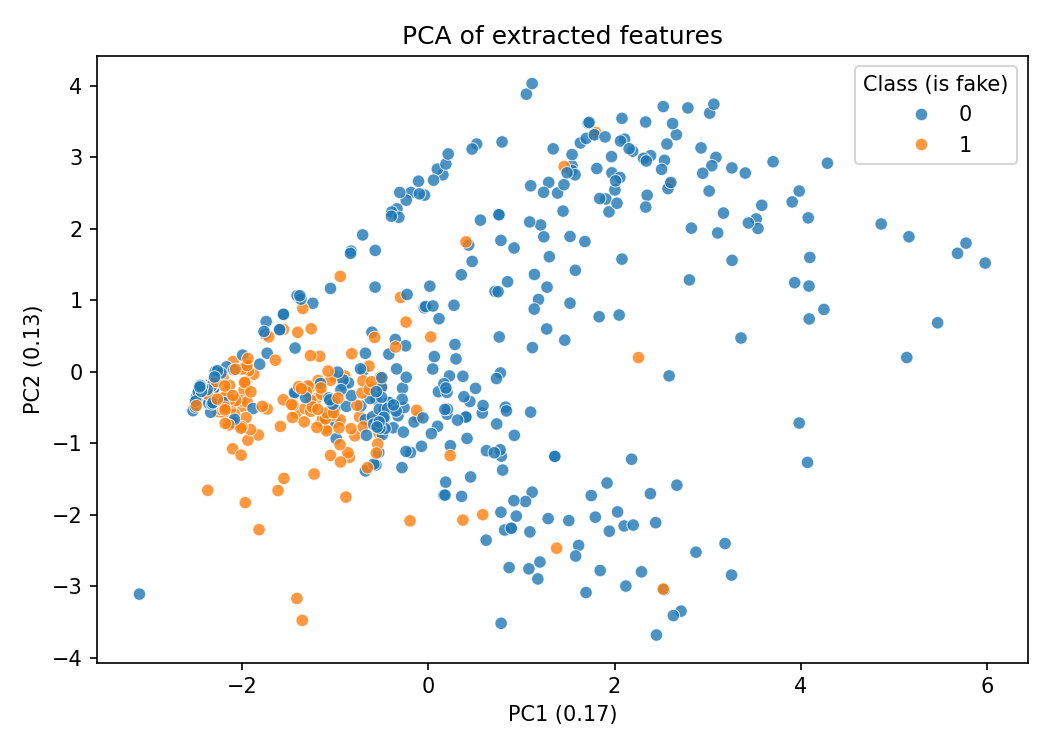
\includegraphics[scale=0.5]{./img/pca_numerical.png}}
	}\\
	\subfigure[t-SNE reduction]{
		{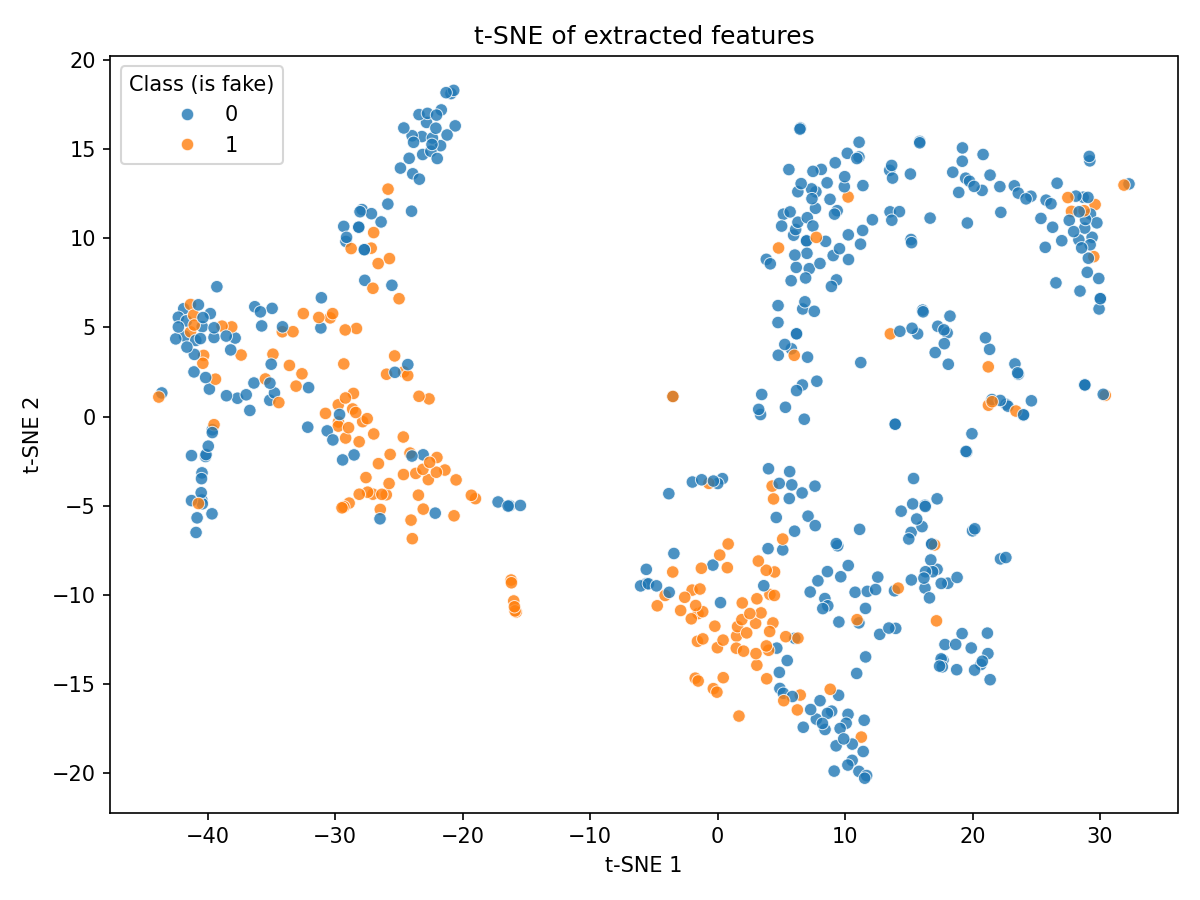
\includegraphics[scale=0.5]{./img/tsne_numerical.png}}
	}
	\vskip -0.5em
	\caption{Dimensionality reduction of numerical data using PCA and t-SNE -- fake news detection}
	\label{fig:numerical_reduction}
	\vspace{-0.1cm}
\end{figure}

As can be seen from these visualizations, especially in the PCA graph, data labeled as fake ($\text{is fake}=1$) tend to be grouped together and very close to each other, unlike data with a negative label, which are much more scattered. This already demonstrates the presence of potentially discriminating factors in the mechanisms of propagation of true and false news on Twitter. It is also likely that a model with non-linear activations and capable of working with large dimensions, such as the bidirectional GRU, can identify patterns that are not visible with a simple PCA.

\subsection{Virality prediction}
\begin{table}[h!]
	\centering
	\caption{Model Performance Comparison on virality prediction (Cross-Validation Averages) -- FakeNewsNet}
	\label{tab:results_fakenewsnet_virality}
	\vspace{0.5em}
	\resizebox{\textwidth}{!}{
	\begin{tabular}{lcccccc}
		\hline
		\textbf{Model} & \textbf{Accuracy} & \textbf{Balanced Acc.} & \textbf{F1} & \textbf{Precision} & \textbf{Recall} & \textbf{ROC AUC} \\
		\hline
		GRU & 0.768 & 0.768 & 0.793 & 0.720 & 0.886 & 0.823 \\
		RNN       & 0.762 & 0.762 & 0.787 & 0.719 & 0.871 & 0.818 \\
		LSTM         & 0.766 & 0.766 & 0.789 & 0.725 & 0.869 & 0.820 \\
		CNN    & 0.770 & 0.770 & 0.790 & 0.731 & 0.864 & 0.830 \\
		Transformer Encoder & 0.776 & 0.776 & \textbf{0.798} & 0.737 & 0.886 & 0.837 \\
		\hline
		Dummy (Stratified)                & 0.500 & 0.500 & 0.000 & 0.000 & 0.000 & 0.500 \\
		Logistic Regression               & 0.691 & 0.691 & 0.695 & 0.687 & 0.705 & 0.768 \\
		Random Forest                     & 0.743 & 0.743 & 0.769 & 0.701 & 0.853 & 0.808 \\
		\hline
	\end{tabular}
}
\end{table}

The results of the different models on the virality prediction task are presented in Table \ref{tab:results_fakenewsnet_virality}. First of all, it is important to note the fundamental difference with respect to the same task on the Evons dataset: in this case, the dataset is perfectly balanced, because the labeling of viral or not-viral posts was based on the median of the data distribution; in the Evons case, on the contrary, the dataset was heavily unbalanced, with the viral class representing only 5\% of the data. For this reason, the scores for this task are generally better, and generally high. In light of these fundamental differences, there are some interesting things to note. Firstly, looking at the baseline models, Logistic Regression performs significantly worse than the other models. This shows the need for non-linear approaches to extract distinctive patterns. We can observe that Random Forest improves on Logistic Regression across all metrics, including recall (0.853 vs. 0.705), confirming its stronger ability to capture complex feature interactions. Logistic Regression remains a useful linear baseline for interpretability, but it is clearly outperformed in this setting.\\

That said, there is a gap between the more complex models and the baseline models, albeit only of around 2-3 F1 points. All the more complex models achieve better scores in F1, precision, and recall. The performances between these models are very close, with the Transformer Encoder achieving slightly better scores. These results confirm what we saw in the fake news detection activity, and therefore the (subtle) superiority of this type of architecture in managing sequential data.

As before, we performed an ablation-like study in order to check the importance of numerical features against text embeddings in predicting virality. We followed the same method explained earlier: we took the first model (GRU) and fed it only the five numerical features once, and only the text embeddings another time. Results are shown in table \ref{tab:results_ablation_virality}

\begin{table}[h!]
	\centering
	\caption{GRU performance comparison on virality prediction with limited input features (Cross-Validation Averages)}
	\vspace{0.5em}
	\label{tab:results_ablation_virality}
	\resizebox{\textwidth}{!}{
		\begin{tabular}{lcccccc}
			\hline
			\textbf{Input data} & \textbf{Accuracy} & \textbf{Balanced Acc.} & \textbf{F1} & \textbf{Precision} & \textbf{Recall} & \textbf{ROC AUC} \\
			\hline
			Only numerical features  & 0.664 & 0.664 & 0.713 & 0.628 & 0.838 & 0.724 \\
			Only BERT emb.           & 0.774 & 0.774 & 0.795 & 0.732 & 0.874 & 0.807 \\
			\hline
			All data                 & 0.768 & 0.768 & 0.793 & 0.720 & 0.886 & 0.823 \\
			\hline
		\end{tabular}
	}
\end{table}

As with fake news detection, the results confirm that textual information provides a strong predictive signal for virality. Using only BERT embeddings, the model achieves an F1 score of 0.80, clearly outperforming the configuration that relies exclusively on numerical features (F1 = 0.71). Nonetheless, the latter still yields competitive performance, especially in terms of recall (0.84), indicating that structural and interaction-based variables -- such as timing, follower counts, or user verification -- capture important dynamics of information diffusion.

Interestingly, unlike in the fake news setting, combining both feature types does not lead to a substantial improvement over text alone. In fact, the model trained on all features attains nearly the same F1 score (0.79), with a slight increase in recall but a small drop in precision. This suggests that while propagation-related metadata carries discriminative information, its contribution partly overlaps with the signal already contained in the textual embeddings. Overall, these findings highlight that virality is strongly correlated with content properties, but that user- and network-level signals also play a meaningful role in shaping diffusion patterns. 

\begin{figure}[h!]
	\centering
	\subfigure[PCA reduction]{
		{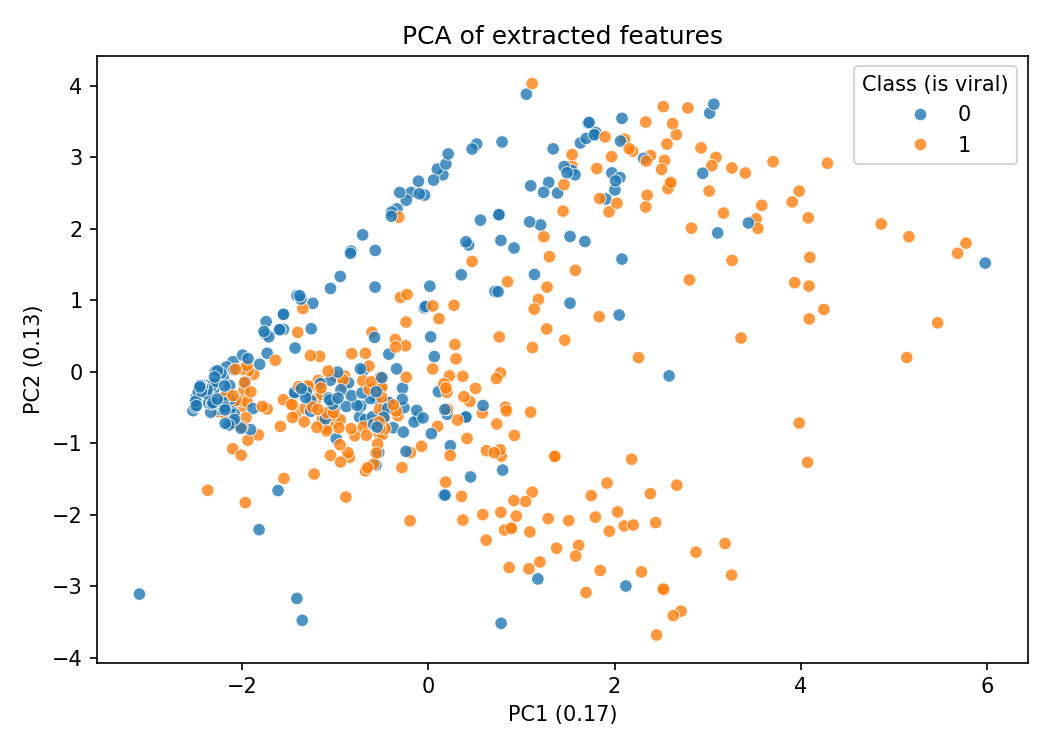
\includegraphics[scale=0.58]{./img/pca_numerical_virality.png}}
	}\\
	\subfigure[t-SNE reduction]{
		{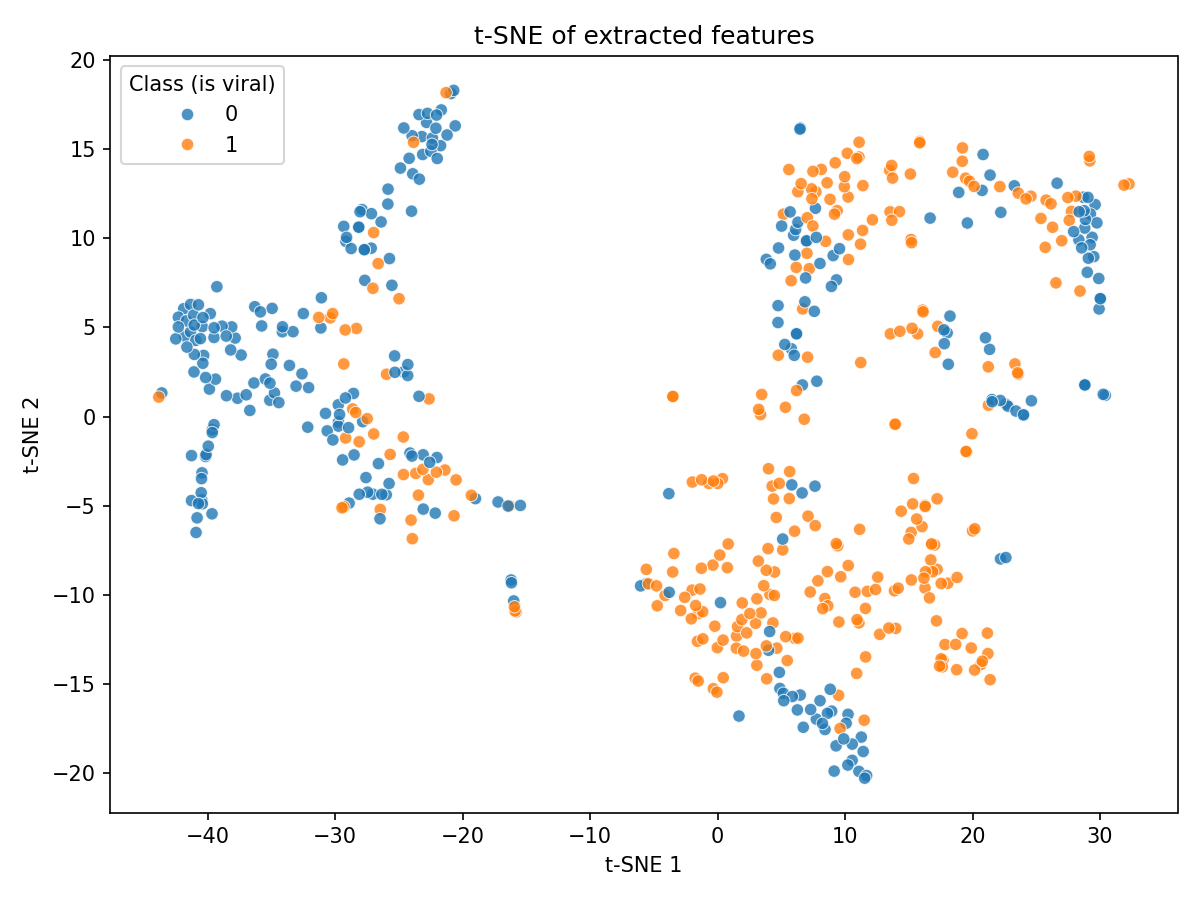
\includegraphics[scale=0.5]{./img/tsne_numerical_virality.png}}
	}
	\vskip -0.5em
	\caption{Dimensionality reduction of numerical data using PCA and t-SNE -- virality prediction}
	\label{fig:numerical_reduction_virality}
	\vspace{-0.1cm}
\end{figure}

As we did previously for fake news detection, we visualized the numerical feature data after reducing its dimensionality using PCA and t-SNE methods. In this case, the data is colored according to the viral or non-viral label. It is interesting to note that in the PCA reduction, the viral and non-viral data points are all very scattered and do not form defined clusters. In contrast, the t-SNE method divided the data into two distinct groups: one overwhelmingly viral, the other the exact opposite. These results are very different from those obtained in fake news detection, where PCA was able to discriminate better than t-SNE. This confirms the greater ability of non-linear methods to capture the discriminating differences between viral and non-viral post sequences, as already suggested by the poor performance of logistic regression compared to other models. 

\FloatBarrier

\subsection{Sequences length}

So far, we have tested all the different models by setting the length of the tweet sequences, $\ell$, equal to 5. One might rightly ask where this choice comes from. The main reason lies in the data itself. In particular, it is worth looking at the descriptive statistics on the lengths of the propagation paths of tweets linked to articles in the FakeNewsNet dataset. In other words, check how long the tweet series are before truncating them or applying padding.This information is available in Table \ref{tab:stats_prop_paths}, which we have also included below for convenience. 
\vspace{1em}
\begin{table}[h!]
	\centering
	\begin{tabular}{lcccccccc}
		\toprule
		Label & Count & Mean & Std & Min & 25\% & 50\% & 75\% & Max \\
		\midrule
		Fake & 174.0 & 400.523 & 1803.121 & 1.0 & 27.0 & 94.5 & 309.50 & 22750.0 \\
		Real & 404.0 & 821.777 & 2189.885 & 1.0 & 8.0 & 56.0 & 759.25 & 21497.0 \\
		\bottomrule
	\end{tabular}
	\caption*{Descriptive statistics of propagation path lengths for Fake and Real labels}
\end{table}

As can be seen, 25\% of the propagation paths associated with a “Real” label have a length less than or equal to 8. Choosing too high a $\ell$ would have reduced the predictive challenge for the models, especially in the task of predicting virality, since a larger proportion of propagation paths would have been fed to the models in their entirety. For this reason, setting $\ell=5$ seemed to be a good balance between a number that was not too high and one that was not too low, allowing the models to capture any interactions between the elements of the sequences. Retrospectively, we verified the appropriateness of this choice. To do so, we studied GRU model's performance as $\ell$ varied, both on fake news detection and on virality prediction tasks. We chose six different possible values for $\ell$: $2, 3, 5, 10, 20, 40$ and we trained the GRU model with the resulting sequences. All hyperparameters were kept constant for better comparison. These scores were obtained using the same cross-validation method explained above, shuffle split cross-validation. For convenience, however, the number of folds was set at 5 instead of the value used so far ($n=10$). Below is a graph and table illustrating the F1-scores obtained.

\pagebreak

\begin{figure}[h!]
	\centering
	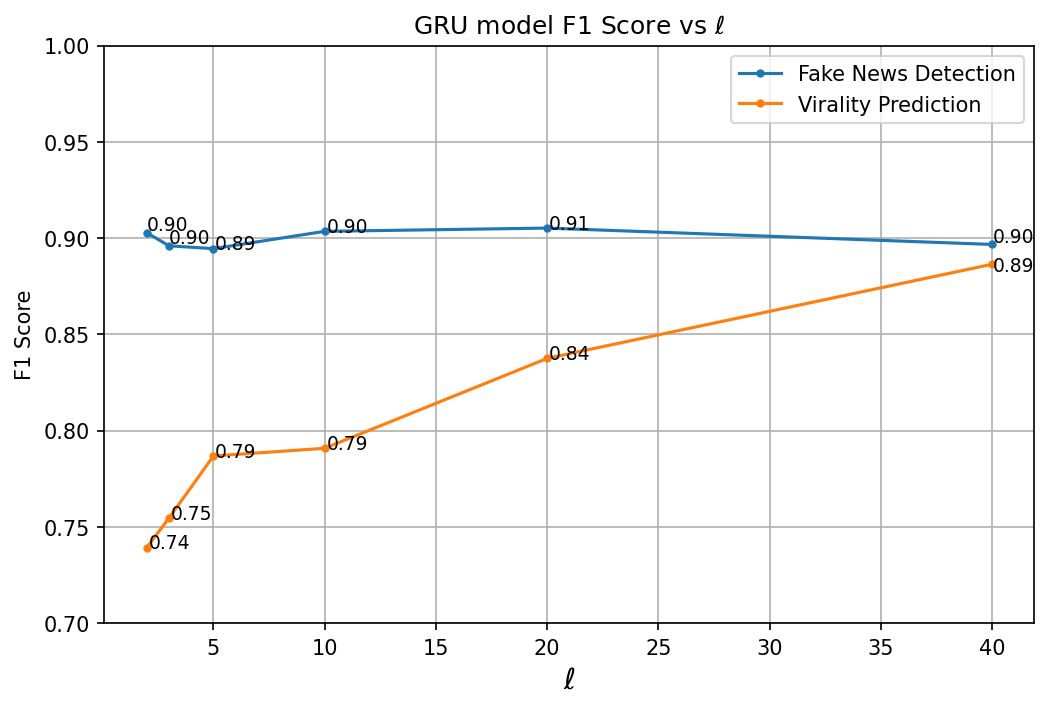
\includegraphics[width=\textwidth]{./img/gru_model_f1_score_vs_l.png}
	\caption{F1 Scores of GRU Model for Fake News Detection and Virality Prediction for different $\ell$ values. \\ \textbf{Note}: y-axis starting at 0.7 for better readability}
\end{figure}

\begin{table}[h!]
	\centering
	\caption{F1 Scores of GRU Model for Fake News Detection and Virality Prediction for different $\ell$ values. In the last row the correlation between $\ell$ and each metric is reported.}
	\begin{tabular}{c|c|c}
		\hline
		\textbf{$\ell$} & \textbf{Fake News Detection F1} & \textbf{Virality Prediction F1} \\
		\hline
		2  & 0.903 & 0.739 \\
		3  & 0.896 & 0.755 \\
		5  & 0.895 & 0.785 \\
		10 & 0.904 & 0.791 \\
		20 & 0.905 & 0.838 \\
		40 & 0.897 & 0.886 \\
		\hline
		\textbf{Corr($\ell$,·)} & -0.029 & {0.965} \\
		\hline
	\end{tabular}
\end{table}
\vspace{1em}

Let's start analyzing results on the fake news detection task. As can be seen, the model's performance remains very similar regardless of the value of $\ell$. This is probably due to the role of the tweet content -- i.e., the embeddings -- which contain the information relevant for classification even in the case of shorter sequences. This is also statistically confirmed, as the Pearson's correlation coefficient between $\ell$ and f1 values on fake news detection is practically 0. It is therefore reasonable to assume that choosing longer or shorter sequences would not have had a significant effect on the models' performance. For the virality prediction task, however, the picture is quite different. The scores vary according to $\ell$. The longer the data sequences, the better the model is able to predict virality. This is obviously not surprising: the longer the data sequences that the model sees during training, the smaller the “portion” of unknown tweets (and likes) that needs to be guessed in order to classify their virality. Let's consider an extreme case to understand this. If the model only took entire, untruncated sequences as input, it would not need to predict anything. It would suffice to add up the number of likes for all tweets contained in the sequences for a perfect classification.\\
This relationship between $\ell$ and the predictive abilities of the model is also demonstrated by the correlation coefficient for the two variables: almost 0.97, i.e., an almost perfect correlation.\\

In light of this, therefore, the choice of $\ell$ has greater implications than in the case of fake news detection. However, the F1 score trend is not constant. Between the scores with $\ell=2$ and $\ell=5$ there is a difference of about 5 f1 points. Between $\ell=5$ and $\ell=10$, however, the difference is much smaller: less than one f1 point. This inconsistent trend can also be seen by observing the line in the graph and can be calculated mathematically as the average slope between the various points, as shown in table \ref{tab:slope_intervals}. As can be seen, the slopes between 2 and 3, and between 3 and 5, are greater than the one in the interval between 5 and 10. This makes the choice of $\ell$=5 even more valid, even in the case of virality prediction.

\begin{table}[h!]
	\centering
	\begin{tabular}{c|c}
		\hline
		\textbf{$\ell$ intervals} & \textbf{Slope} \\
		\hline
		2 -- 3   & 1.530 \\
		3 -- 5   & 1.615 \\
		5 -- 10  & 0.080 \\
		10 -- 20 & 0.467 \\
		20 -- 40 & 0.245 \\
		\hline
	\end{tabular}
	\caption{Slope values across different intervals}
	\label{tab:slope_intervals}
\end{table}

\clearpage

\section{A note on the embedding strategy}
We have presented the results for both datasets and both tasks. At this point, before moving on to the general conclusions, it is important to focus on another aspect that concerns all the models used in this work. All the text embeddings mentioned so far were created with \texttt{RoBERTa}. Although generally considered a good model, it is not necessarily the best or the state-of-the-art. It is perfectly plausible that different embedding techniques could yield different, potentially better, performances. Clearly, it would be impossible to verify this option by trying all possible embedding techniques and comparing the results. For the sake of completeness, however, we did a test using different embeddings at least once on both datasets and for both tasks. We did this using Mistral's API service, which allows texts to be transformed into 1024-dimensional numerical vectors. This is 256 dimensions more than \texttt{RoBERTa}'s embeddings, which could allow for a more accurate representation of linguistic nuances and meaning.\\

Specifically, we used the following models for comparison: for the EVONS dataset, the MLP model for fake news detection and the gating model for virality prediction; for the FakeNewsNet dataset, the GRU model in both tasks. Table \ref{tab:results_mistral_bert} shows in detail the results obtained with Mistral embeddings. For easier comparison, the scores obtained with \texttt{RoBERTa} embeddings are shown in parentheses. Here below, instead, a condensed version of the same table, showing only F1 score:

\begin{table}[H]
	\centering
	\caption*{Comparative F1 scores (Mistral vs. \texttt{RoBERTa}). Values are reported as Mistral (\texttt{RoBERTa}).}
	\label{tab:f1_mistral_bert}
	\begin{tabular}{llc}
		\toprule
		\textbf{Task} & \textbf{Dataset} & \textbf{F1 Score} \\
		\midrule
		Fake News Detection & EVONS       & 0.992 (0.990) \\
		Fake News Detection & FakeNewsNet & 0.906 (0.891) \\
		Virality Prediction & EVONS       & 0.337 (0.323) \\
		Virality Prediction & FakeNewsNet & 0.773 (0.793) \\
		\bottomrule
	\end{tabular}
\end{table}

The comparison shows that the differences between Mistral and \texttt{RoBERTa} embeddings are generally small and do not alter the overall picture. On EVONS -- fake news detection, results are already close to perfect, and the improvements from Mistral are negligible (F1 0.992 vs 0.990). On FakeNewsNet -- fake news detection, the gains are slightly more visible (F1 0.906 vs 0.891, ROC AUC 0.972 vs 0.961), but still modest in scale. For EVONS -- virality prediction, Mistral brings a minor increase in F1 (0.337 vs 0.323) and Recall, while for FakeNewsNet -- virality prediction \texttt{RoBERTa} performs a little better (F1 0.773 vs 0.793). In fact, absolute changes in F1 across all comparisons never exceed 0.02, confirming that the observed differences are marginal. Taken together, these results show that alternative embeddings can shift scores slightly, but the changes are too small to affect the main conclusions of this work.

\begin{sidewaystable}[htbp]
	\centering
	\caption{Comparative results (Mistral vs. \texttt{RoBERTa}). Values are reported as Mistral (\texttt{RoBERTa}).}
	\label{tab:results_mistral_bert}
	\begin{tabular}{lllcccccc}
		\toprule
		\textbf{Task} & \textbf{Dataset} & \textbf{Model} & \textbf{Accuracy} & \textbf{Balanced Acc.} & \textbf{F1} & \textbf{Precision} & \textbf{Recall} & \textbf{ROC AUC} \\
		\midrule
		Fake News Detection & EVONS       & MLP    & 0.992 (0.991) & 0.992 (0.991) & 0.992 (0.990) & 0.993 (0.990) & 0.991 (0.990) & 1.000 (0.999) \\
		Fake News Detection & FakeNewsNet & GRU    & 0.945 (0.935) & 0.927 (0.918) & 0.906 (0.891) & 0.933 (0.912) & 0.883 (0.874) & 0.972 (0.961) \\
		Virality Prediction & EVONS       & Gating model & 0.866 (0.869) & 0.779 (0.751) & 0.337 (0.323) & 0.225 (0.219) & 0.682 (0.620) & 0.886 (0.868) \\
		Virality Prediction & FakeNewsNet & GRU    & 0.753 (0.768) & 0.753 (0.768) & 0.773 (0.793) & 0.720 (0.720) & 0.840 (0.886) & 0.816 (0.823) \\
		\bottomrule
	\end{tabular}
\end{sidewaystable}


\chapter{Conclusions}

This chapter will present the conclusions of this work, during which experiments were carried out on different data and different activities. For this reason, it is best to proceed in an orderly fashion. The chapter is structured as follows: first, we will draw conclusions for the different datasets and activities, thus imitating the structure of the previous chapters. Next, we will report any general conclusions. Along with the conclusions, the numerous limitations of this work will also be presented. \\
Before looking at the conclusions for individual datasets and activities, a general limitation of our model evaluation protocol should be noted. For each fold, we selected the best epoch based on performance on the corresponding test fold \footnote{For greater details, see the \hyperref[annex]{annex}}. This procedure can inflate reported results, since the test set is ideally reserved only for final evaluation. The more rigorous alternative would be to hold out a separate validation set within each fold (train–validation–test) and select the epoch using validation performance. However, the FakeNewsNet dataset contains relatively few cascades, making such a three-way split impractical without severely reducing the amount of training data. For consistency, we applied the same protocol to the larger Evons dataset. While this choice may slightly overestimate absolute scores, it does not affect the relative comparisons between models or the main conclusions of this work, which rely on consistent cross-dataset trends rather than absolute metric values\footnote{For verification purposes, we conducted a trial on the Evons dataset, on the task of predicting virality, using the more rigorous train-validation-test division protocol. The result is an average f1 of 0.303 on the test set across ten folds: only one point difference compared to the performances obtained previously. This highlights the marginality of the inflation effect on metrics.}.

\section{Evons}
Before moving on to the individual tasks, a general note should be made. The data used was collected on Facebook between 2016 and 2017, almost ten years ago. During this time, many things have changed in the way this platform works and the way users use it. For example, in January 2025, at the beginning of Trump's term as US president, Meta announced a major shift in its content moderation strategy\footcite{paul2025}: it ended its partnerships with third-party fact-checkers and introduced a crowdsourced “community notes” model. The company also reversed earlier efforts to downrank political content, instead promising to boost its visibility, while relaxing restrictions on sensitive topics like gender and immigration. These developments illustrate how significantly Meta’s approach to information governance and user engagement has evolved over time. 

This represents a limitation of this work and requires caution when drawing any conclusions based on this data.

\subsection{Fake news detection}
Let's start with the obvious: there is not much to say about the results obtained for fake news detection on the Evons dataset. All models work well, except, of course, the Dummy. The only thing worth noting is the ability of the embeddings created by \texttt{RoBERTa} to extract textual features that are so significant that even a linear model achieves excellent results. \\
There is much to say, however, about the relevance of identifying fake news with this approach. It is a classification that risks being misleading for several reasons. First, the binary true/false label is reductive given the complexity of the real information landscape: it is no coincidence that many journalistic fact-checking services use more nuanced categories, such as “partially true,” “partially false,” and so on. Additionally, the manner in which these labels were extracted is problematic. Categorizing the truth or falsehood of a news item based solely on its source without independent fact-checking is an effective but risky shortcut. The most dangerous disinformation narratives are those that reach major newspapers, not those that remain in obscure corners of the internet. Similarly, assuming that everything from a certain publication is false is equally wrong. For example, at the time of writing, the opening article on The People's Voice website -- the successor to Your News Wire, a source of fake news in the Evons dataset -- is titled \enquote{Trump Says World Doesn't Need to Worry About WW3 Anymore}\footnote{\url{https://web.archive.org/web/20250821104858/https://thepeoplesvoice.tv/}. Coincidentally, a new article was published just as the Wayback Machine was acquiring the page. Therefore, the article used as an example is the second one from the top.}. The article cites RT, a media outlet widely regarded as a mouthpiece for Russian propaganda. RT, in turn, refers to a statement made by Trump during a recent episode of conservative journalist Mark Levin's podcast. The recording is available on YouTube, and it is easy to verify that the statement was made at around the 18-minute mark\footnote{\url{https://youtu.be/qh_34L3lov8?si=DlIUiOsSdabVtSpw&t=1115}}. Therefore, the article is fundamentally true, even if it lacks context and critical commentary.\\

Finally, this labeling approach also creates the risk of a \emph{source confound}: the model can learn to recognize stylistic or lexical patterns that uniquely identify certain outlets, and then simply associate those outlets with a truth value, rather than actually evaluating the veracity of the article’s content. In practice, this means that part of the very high accuracy achieved may come not from detecting disinformation cues, but from identifying which outlet produced the text. While this problem could inflate performance on Evons, it is worth noting that the same architectures also perform strongly on the FakeNewsNet dataset, where labels are assigned at the article level by fact-checkers. This reduces the likelihood of a dramatic performance drop and suggests that the models are indeed capturing content-related signals as well. Nevertheless, the methodological lesson is clear: labeling news as true or false should always be based on the content, not on the source.

For all these reasons, despite the models tested performing well, it is difficult to argue that they can actually be used in a disinformation identification pipeline.

\subsection{Virality prediction}
Here too, we can start with the obvious: all models are generally unsatisfactory. Regardless of the architecture used, the scores remain low. This clearly shows how difficult it is to use traditional machine learning methods with heavily imbalanced datasets, where the positive class is present in only one out of twenty cases. This is particularly true when faced with non-trivial tasks such as predicting virality. The result is a classic trade-off between precision and recall in classification. This raises important questions about the model evaluation method itself: is it better to have a model with a better balance between precision and recall, when it is known that the former will not exceed 0.3 and the latter 0.65, or a model with very low precision -- less than 0.15 -- but a recall of over 0.8? The answer is not obvious and depends on the specific needs of the application in question.

Realistically, in a pipeline for identifying disinformation at risk of going viral, a model similar to the second would be preferable. This would enable a significant proportion of the incoming data to be filtered with the assurance that hardly any relevant information is being lost. Although insufficient, therefore, a model of this type could still be useful. However, it could only serve as the first step in a longer processing chain involving further analysis of elements classified as potentially viral in order to obtain more accurate results. In other words, such a model alone would not be sufficient. This highlights the need to study more sophisticated methods and collect higher-quality data to address the problem of predicting virality in a highly unbalanced context.

\section{FakeNewsNet}
Moving on to the FakeNewsNet dataset, we must first address a general issue. This data was obtained through the collaboration of one university researcher who agreed to share it without asking for anything in return. Such an approach was necessary because the Twitter/X API is now inaccessible without paying large sums of money.
Consequently, we ended up with a dataset about which we have little information. For instance, we don't know when the data was downloaded from the API. Additionally, the data is potentially corrupted; all retweets have 0 likes, which is highly unlikely. Consequently, we had to discard them in our analysis, which greatly reduced the amount of available data. This represents a strong limit of this work.

At the risk of sounding trite, it's important to remember the necessity of making data accessible for social science research, especially on social media, while respecting user privacy. In the absence of institutional guarantees, much of the research on this topic depends on the goodwill of large companies in the sector, which can change their minds and close access at any moment, with no accountability, as recent events have shown.

\subsection{Fake news detection}

All models used for the fake news detection task on FakeNewsNet data perform well. The results are very good despite the modest amount of data available for training and the imbalance in the dataset, which sees the positive class present in 30\% of cases. This demonstrates that data imbalance is not always problematic, but rather, only when the task itself is particularly challenging, as in the case of virality prediction.

The results of models that use only a certain type of data as input are particularly interesting: textual content in one case and numerical features in another, such as the number of likes on tweets, the number of followers of the user, the time elapsed since the first publication, and other variables defined in the \hyperref[Methods]{Methods} section. It is clear that identifying fake news based on textual content works very well on its own. Therefore, it is the texts that carry the greatest amount of useful discriminating signals for classification. However, the results using only numerical features are also encouraging. Although not perfect, they show that it is possible to use exclusively numerical data to identify fake news. This approach is especially helpful when dealing with languages that are not as prevalent as European languages, as language models like BERT are not available for them. Additionally, the creation of large amounts of textual embeddings requires a significant amount of computing power, which can lead to issues when resources are scarce.

Researchers could further investigate identifying fake news using non-textual signals, which could lead to the creation of more effective models, for example by trying to integrate a greater number of features.

\subsection{Virality prediction}

First, it's important to note that, unlike the EVONS dataset, the dataset in this case was perfectly balanced based on how virality was defined. This helped achieve fairly high results for all models. Despite the balance, however, performance was generally worse than that observed in fake news detection. This further confirms the greater intrinsic difficulty of predicting virality compared to fake news detection. This is understandable, as the virality of a post can depend on many factors, including those external to social media itself. Therefore, methods capable of integrating a greater variety of data to predict virality should be explored to highlight relevant interactions not taken into account until now.

Regarding the contribution of different types of features to prediction quality, our experiments showed that eliminating textual content information results in smaller performance deterioration than in fake news detection. Therefore, this also suggests the possibility of developing methods for predicting virality that are not dependent on the content of publications.

Another important aspect to highlight is the difference in the quality of PCA and t-SNE clustering on the numerical features of the data. The latter works much better than the former, indicating that non-linearity finds relevant hidden patterns within the data. This is also confirmed by the performance of the different models. Studying the patterns identified by nonlinear operations could help us understand which aspects allow for better classification results. Such a study could provide useful information for more informed feature extraction from raw data. \\

Finally, it is important to highlight some limitations in the way this task was designed. Due to the limited amount of data available, we defined virality based on the median distribution of likes obtained by the series of tweets. In fact, this corresponds to using a rather low absolute value (less than 50 likes) as a threshold, which can hardly be considered an index of virality according to its common meaning. This obviously represents a limitation of this study. In addition, another potential limitation concerns the use of likes as predictive features: ideally, the number of likes should be censored with respect to a fixed time horizon (for example, the first six or twelve hours after publication), in order to avoid introducing information that would not have been available at prediction time. However, this kind of strict time-censoring is extremely difficult to implement in practice given the very limited and costly access to complete social media archives. For this reason, likes have been treated here as pragmatic proxies of early engagement, while leaving to future work the possibility of more precise modeling once richer data become available.

\section{General conclusions}
In light of what has been said so far, some general conclusions can be drawn.

First, this work demonstrates that fake news can be successfully identified based on textual content and other data. Almost all of the models created in this study perform well. However, there is a high risk that these models only work for the most obvious and striking cases of disinformation. It is unclear how these models would behave when faced with borderline cases of news that is not entirely false but rather distorted or taken out of context. For this reason, it is important to emphasize the need for better datasets to study methods for identifying fake news. We need data that goes beyond the most obvious cases and uses more granular categories suited to the complexity of the real world instead of simple binary labels. Therefore, there is a clear need to make social media data more accessible for research.

In addition to this, the current study highlighted the difficulties faced by many types of machine learning models in obtaining satisfactory results with highly imbalanced datasets. This is a problem that has not yet been fully resolved by research on the subject, for which there are not always effective solutions. Nevertheless, it has been shown that even imperfect models can be useful in the context of a realistic pipeline for identifying viral disinformation content, albeit insufficiently so. Further research is needed to develop more sophisticated methods that can integrate other types of data and contextual information that may be relevant for determining virality.

Finally, a note that stems from the underlying spirit of this work. Global concern about disinformation, and in particular about disinformation narratives that reach a large audience, stems from a simple idea: people can change their behavior and opinions when exposed to such content. However, measuring the real effect of disinformation campaigns on people's behavior is very complicated, because it can depend on many different factors. This represents a huge gap in our knowledge on the subject, which is difficult to resolve using computational methods alone, and is perhaps one of the most urgent issues to address.

\appendix
\part*{Annex} \label{annex}
\addcontentsline{toc}{part}{Annex}
\chapter*{Code logic and explanation}
\addcontentsline{toc}{chapter}{Code logic and explanation}

This section illustrates some technical aspects of the codes used to train the models examined in this work. The code and the data are available here: \url{https://github.com/savaij/memoire_disinfo}

\section*{Metrics logging}

First, a note on metrics. During the training cycles, at each epoch, performance is recorded online via the \emph{Weights \& Biases} platform -- specifically, its python library \emph{wandb} -- and grouped for each fold. This made it possible to store the metric data and reuse it for detailed post-hoc analysis -- for example, the evolution of performance based on the definition of the $F\text{-}\beta$ score (Figure \ref{fig:ratios}).

\begin{figure}[h!]
	\centering
	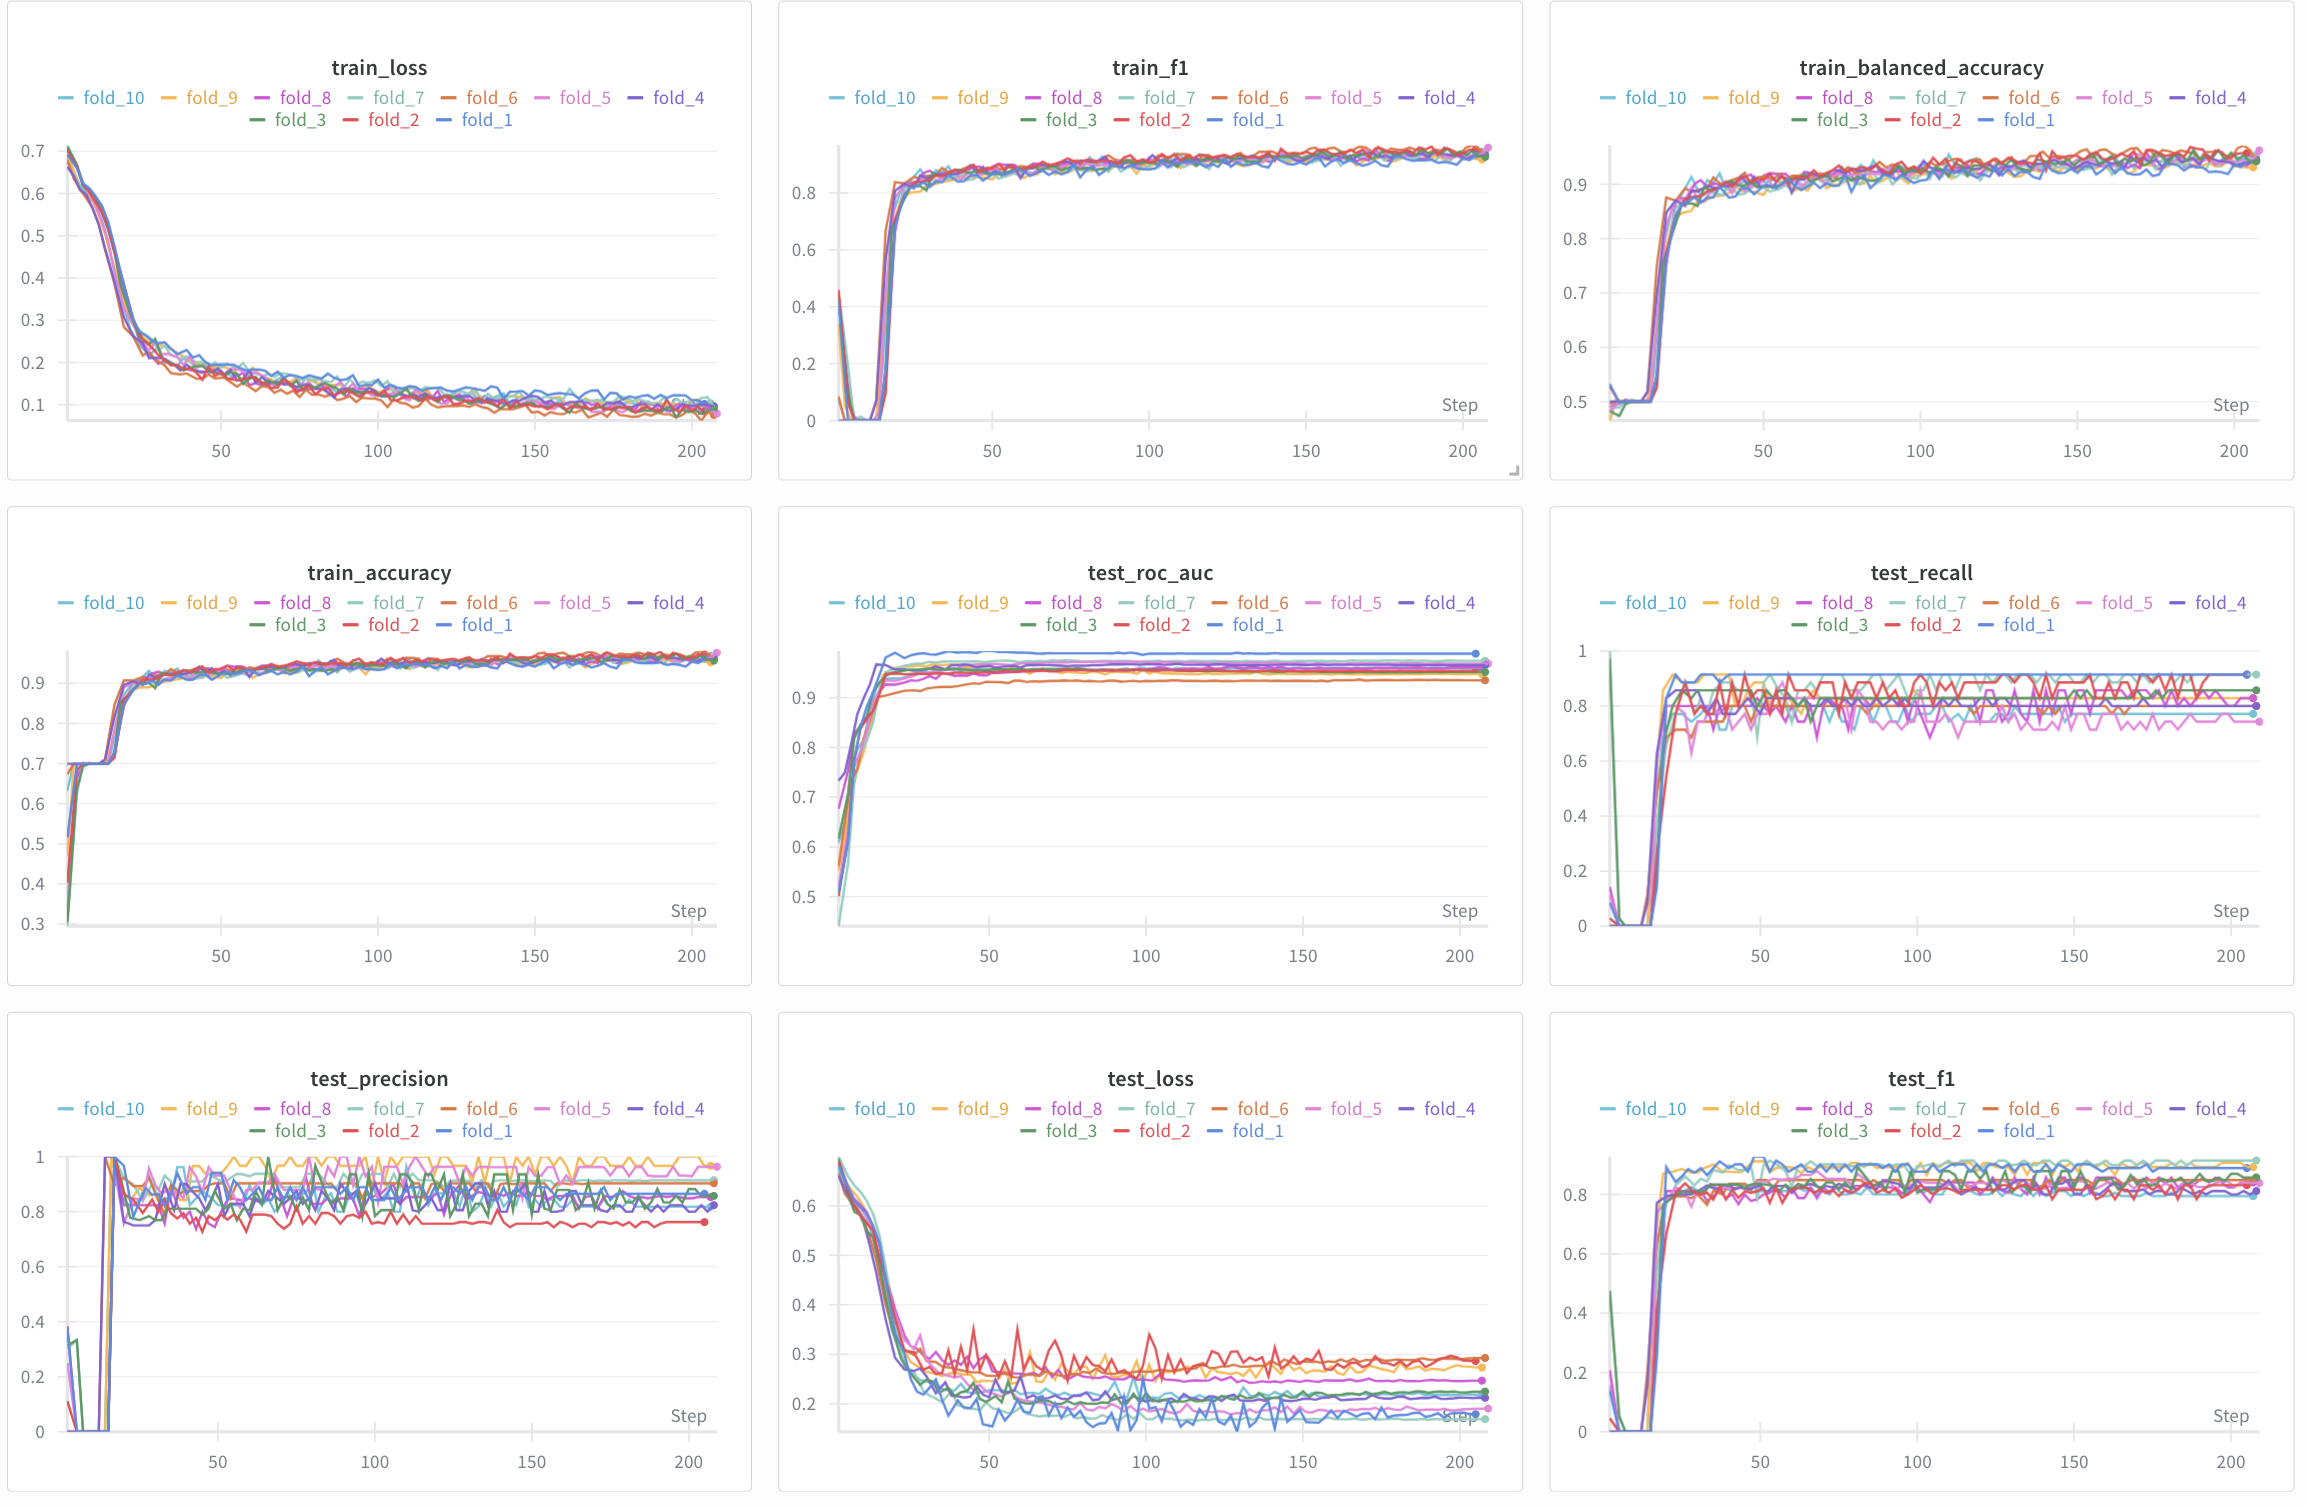
\includegraphics[width=\textwidth]{./img/wandb_screenshot.png}
	\caption{Screenshot of monitoring data during training on \emph{wandb}}
\end{figure}

All codes and models are built with the \emph{PyTorch} library.

\section*{Code structure}

The training codes, in the form of Jupyter notebooks, share the same basic structure, with minor variations depending on the datasets and the specific tasks.  

\paragraph{First step.} Naturally, the first element of the structure is data acquisition and preprocessing. This essentially consists of loading the previously created textual embeddings and synchronizing them with other types of data. In certain cases, a preprocessing function is also defined to be applied within each fold, i.e., after defining the training and test sets -- for example, the normalization defined in \ref{fakenewsdata_detection_models}.  

\paragraph{Second step.} The second step consists of defining the architecture of the model under consideration.  

\paragraph{Third step.} The third step involves creating the functions to be used within each training cycle. A function is created for the model’s test loop, which computes and returns its metrics. Subsequently, a function is created that encapsulates the core of training for a single fold: within this function, the training and test sets are defined, the model is initialized, and the training loop is executed. Metrics from each epoch are logged online, while within the loop the metrics of the epoch with the best F1 score on the test set are stored. These are then returned by the function itself. Here below is a simplified pseudo-code version of the single fold function to show the key steps.

\clearpage


\begin{algorithm}[H]
	\caption{Train a Single Fold}
	\begin{algorithmic}
		\Function{TrainSingleFold}{train indices, validation indices, features, labels}
		\Statex \vspace{0.5em}
		\Comment{--- Data preparation ---}
		\State \textbf{Split features} into train and validation sets using corresponding indices
		\State \textbf{Extract labels} for train and validation using corresponding indices
		\State \textbf{Create dataset and dataloaders} objects for train and validation
		
		\Statex \vspace{0.5em}
		\Comment{--- Model setup ---}
		\State \textbf{Initialize model}
		\State \textbf{Define optimizer, loss, and scheduler}
		\State \textbf{Initialize} best\_metrics $\gets$ None, best\_f1 $\gets 0$

		\Statex \vspace{0.5em}
		\Comment{--- Training loop ---}
		\For{each epoch in total epochs}
		\State \textbf{Train} model for one epoch
		\State \textbf{Evaluate} on training data (logging metrics)
		\State \textbf{Evaluate} on validation data (logging metrics)
		\If{validation F1 $>$ best\_f1}
		\State \textbf{Update} best\_f1 and best\_metrics
		\EndIf
		\EndFor
	
		\State \Return best\_metrics
		
		\EndFunction
	\end{algorithmic}
\end{algorithm}


\paragraph{Fourth step.} The fourth step is the implementation of the cross-validation loop, which coordinates the entire training and evaluation process. This function creates an additional loop in which, for each fold, the training function defined in the previous step is called and the metrics are stored. At the end of all folds, summary statistics (mean and standard deviation) are computed for all relevant metrics.  The logic behind the function can be illustrated in a simplified version in the pseudo-code here below.

\clearpage

\begin{algorithm}[H]
	\caption{Run 10-Fold Cross-Validation}
	\begin{algorithmic}
		\Function{RunCrossValidation}{config parameters}
		
		\Statex \vspace{0.5em}
		\Comment{--- Initialize Cross-Validation ---}
		\State \textbf{Initialize} CrossValidationSplit with 10 folds
		\State \textbf{Initialize} all\_best\_metrics $\gets$ empty list
		
		\Statex \vspace{0.5em}
		\Comment{--- Train Each Fold ---}
		\For{fold, (train\_indices, val\_indices) in CrossValidationSplit}
		\State best\_fold\_metrics $\gets$ \Call{TrainSingleFold}{train indices, validation indices, features, labels}
		\State \textbf{Append} best\_fold\_metrics to all\_best\_metrics
		\EndFor
		
		\Statex \vspace{0.5em}
		\Comment{--- Summary Statistics ---}
		\State \textbf{Print} Cross-validation summary (all\_best\_metrics mean values and standard deviation)
		
		\State \Return all\_best\_metrics
		\EndFunction
	\end{algorithmic}
\end{algorithm}

\section*{Hyperparameters}

As already mentioned earlier, in this work no extensive search for the best combination of hyperparameters for training the models was carried out. A few combinations were tested manually. Once a satisfactory selection was identified, it was kept identical across models of the same family in order to enable a more rigorous performance comparison. All models use a scheduler for the linear decrease of the learning rate during training. No early stopping mechanism was implemented. The parameters used are detailed below.

For the tasks related to the Evons dataset, all models use the hyperparameters reported in Table \ref{tab:mlp-hparams}.

\begin{table}[H]
	\centering
	\begin{tabular}{ll}
		\toprule
		\textbf{Parameter} & \textbf{Value} \\
		\midrule
		Learning rate & $1 \times 10^{-4}$ \\
		Weight decay & $0.01$ \\
		Dropout & $0.1$ \\
		Number of epochs & $50$ \\
		\bottomrule
	\end{tabular}
	\caption{Hyperparameters used for training models on tasks on Evons dataset.}
	\label{tab:mlp-hparams}
\end{table}

The hyperparameters used for the tasks on the FakeNewsNet dataset are shown in Table~\ref{tab:fakenews-hparams}.

\begin{table}[H]
	
	\centering
	
	\begin{tabular}{ll}
		
		\toprule
		
		\textbf{Parameter} & \textbf{Value} \\
		
		\midrule
		
		Learning rate & $8 \times 10^{-5}$ \\
		
		Weight decay & $0.01$ \\
		
		Dropout & $0.1$ \\
		
		Number of epochs & $100$ \\
		
		\bottomrule
		
	\end{tabular}
	
	\caption{Hyperparameters used for training the models on the FakeNewsNet dataset.}
	
	\label{tab:fakenews-hparams}
	
\end{table}

The models related to FakeNewsNet data were trained with a lower learning rate but a much higher number of epochs compared to the models trained on the Evons dataset. Experiments showed that this setup consistently led to slightly better performance across all models. However, further analysis is needed to fully understand why this happens. One possible explanation is the difference in the number of data points between the Evons and FakeNewsNet datasets.\\
 In the codes used, some parameters also concern the dimensionality of the projections in the hidden layers of the various models. These were not included among the hyperparameters shown above. The chosen dimensions are those reported in the \hyperref[Methods]{Methods} section.

\printbibliography

\tableofcontents
\listoffigures

\end{document}
	